% Options for packages loaded elsewhere
\PassOptionsToPackage{unicode}{hyperref}
\PassOptionsToPackage{hyphens}{url}
\PassOptionsToPackage{dvipsnames,svgnames,x11names}{xcolor}
%
\documentclass[
  a4paper,
  DIV=11,
  numbers=noendperiod,
  onepage,
  openany]{scrreprt}

\usepackage{amsmath,amssymb}
\usepackage{iftex}
\ifPDFTeX
  \usepackage[T1]{fontenc}
  \usepackage[utf8]{inputenc}
  \usepackage{textcomp} % provide euro and other symbols
\else % if luatex or xetex
  \usepackage{unicode-math}
  \defaultfontfeatures{Scale=MatchLowercase}
  \defaultfontfeatures[\rmfamily]{Ligatures=TeX,Scale=1}
\fi
\usepackage{lmodern}
\ifPDFTeX\else  
    % xetex/luatex font selection
\fi
% Use upquote if available, for straight quotes in verbatim environments
\IfFileExists{upquote.sty}{\usepackage{upquote}}{}
\IfFileExists{microtype.sty}{% use microtype if available
  \usepackage[]{microtype}
  \UseMicrotypeSet[protrusion]{basicmath} % disable protrusion for tt fonts
}{}
\makeatletter
\@ifundefined{KOMAClassName}{% if non-KOMA class
  \IfFileExists{parskip.sty}{%
    \usepackage{parskip}
  }{% else
    \setlength{\parindent}{0pt}
    \setlength{\parskip}{6pt plus 2pt minus 1pt}}
}{% if KOMA class
  \KOMAoptions{parskip=half}}
\makeatother
\usepackage{xcolor}
\usepackage[lmargin=30mm,rmargin=30mm,tmargin=35mm,bmargin=30mm]{geometry}
\setlength{\emergencystretch}{3em} % prevent overfull lines
\setcounter{secnumdepth}{5}
% Make \paragraph and \subparagraph free-standing
\ifx\paragraph\undefined\else
  \let\oldparagraph\paragraph
  \renewcommand{\paragraph}[1]{\oldparagraph{#1}\mbox{}}
\fi
\ifx\subparagraph\undefined\else
  \let\oldsubparagraph\subparagraph
  \renewcommand{\subparagraph}[1]{\oldsubparagraph{#1}\mbox{}}
\fi

\usepackage{color}
\usepackage{fancyvrb}
\newcommand{\VerbBar}{|}
\newcommand{\VERB}{\Verb[commandchars=\\\{\}]}
\DefineVerbatimEnvironment{Highlighting}{Verbatim}{commandchars=\\\{\}}
% Add ',fontsize=\small' for more characters per line
\usepackage{framed}
\definecolor{shadecolor}{RGB}{241,243,245}
\newenvironment{Shaded}{\begin{snugshade}}{\end{snugshade}}
\newcommand{\AlertTok}[1]{\textcolor[rgb]{0.68,0.00,0.00}{#1}}
\newcommand{\AnnotationTok}[1]{\textcolor[rgb]{0.37,0.37,0.37}{#1}}
\newcommand{\AttributeTok}[1]{\textcolor[rgb]{0.40,0.45,0.13}{#1}}
\newcommand{\BaseNTok}[1]{\textcolor[rgb]{0.68,0.00,0.00}{#1}}
\newcommand{\BuiltInTok}[1]{\textcolor[rgb]{0.00,0.23,0.31}{#1}}
\newcommand{\CharTok}[1]{\textcolor[rgb]{0.13,0.47,0.30}{#1}}
\newcommand{\CommentTok}[1]{\textcolor[rgb]{0.37,0.37,0.37}{#1}}
\newcommand{\CommentVarTok}[1]{\textcolor[rgb]{0.37,0.37,0.37}{\textit{#1}}}
\newcommand{\ConstantTok}[1]{\textcolor[rgb]{0.56,0.35,0.01}{#1}}
\newcommand{\ControlFlowTok}[1]{\textcolor[rgb]{0.00,0.23,0.31}{#1}}
\newcommand{\DataTypeTok}[1]{\textcolor[rgb]{0.68,0.00,0.00}{#1}}
\newcommand{\DecValTok}[1]{\textcolor[rgb]{0.68,0.00,0.00}{#1}}
\newcommand{\DocumentationTok}[1]{\textcolor[rgb]{0.37,0.37,0.37}{\textit{#1}}}
\newcommand{\ErrorTok}[1]{\textcolor[rgb]{0.68,0.00,0.00}{#1}}
\newcommand{\ExtensionTok}[1]{\textcolor[rgb]{0.00,0.23,0.31}{#1}}
\newcommand{\FloatTok}[1]{\textcolor[rgb]{0.68,0.00,0.00}{#1}}
\newcommand{\FunctionTok}[1]{\textcolor[rgb]{0.28,0.35,0.67}{#1}}
\newcommand{\ImportTok}[1]{\textcolor[rgb]{0.00,0.46,0.62}{#1}}
\newcommand{\InformationTok}[1]{\textcolor[rgb]{0.37,0.37,0.37}{#1}}
\newcommand{\KeywordTok}[1]{\textcolor[rgb]{0.00,0.23,0.31}{#1}}
\newcommand{\NormalTok}[1]{\textcolor[rgb]{0.00,0.23,0.31}{#1}}
\newcommand{\OperatorTok}[1]{\textcolor[rgb]{0.37,0.37,0.37}{#1}}
\newcommand{\OtherTok}[1]{\textcolor[rgb]{0.00,0.23,0.31}{#1}}
\newcommand{\PreprocessorTok}[1]{\textcolor[rgb]{0.68,0.00,0.00}{#1}}
\newcommand{\RegionMarkerTok}[1]{\textcolor[rgb]{0.00,0.23,0.31}{#1}}
\newcommand{\SpecialCharTok}[1]{\textcolor[rgb]{0.37,0.37,0.37}{#1}}
\newcommand{\SpecialStringTok}[1]{\textcolor[rgb]{0.13,0.47,0.30}{#1}}
\newcommand{\StringTok}[1]{\textcolor[rgb]{0.13,0.47,0.30}{#1}}
\newcommand{\VariableTok}[1]{\textcolor[rgb]{0.07,0.07,0.07}{#1}}
\newcommand{\VerbatimStringTok}[1]{\textcolor[rgb]{0.13,0.47,0.30}{#1}}
\newcommand{\WarningTok}[1]{\textcolor[rgb]{0.37,0.37,0.37}{\textit{#1}}}

\providecommand{\tightlist}{%
  \setlength{\itemsep}{0pt}\setlength{\parskip}{0pt}}\usepackage{longtable,booktabs,array}
\usepackage{calc} % for calculating minipage widths
% Correct order of tables after \paragraph or \subparagraph
\usepackage{etoolbox}
\makeatletter
\patchcmd\longtable{\par}{\if@noskipsec\mbox{}\fi\par}{}{}
\makeatother
% Allow footnotes in longtable head/foot
\IfFileExists{footnotehyper.sty}{\usepackage{footnotehyper}}{\usepackage{footnote}}
\makesavenoteenv{longtable}
\usepackage{graphicx}
\makeatletter
\def\maxwidth{\ifdim\Gin@nat@width>\linewidth\linewidth\else\Gin@nat@width\fi}
\def\maxheight{\ifdim\Gin@nat@height>\textheight\textheight\else\Gin@nat@height\fi}
\makeatother
% Scale images if necessary, so that they will not overflow the page
% margins by default, and it is still possible to overwrite the defaults
% using explicit options in \includegraphics[width, height, ...]{}
\setkeys{Gin}{width=\maxwidth,height=\maxheight,keepaspectratio}
% Set default figure placement to htbp
\makeatletter
\def\fps@figure{htbp}
\makeatother

\KOMAoption{captions}{tableheading}
\makeatletter
\@ifpackageloaded{tcolorbox}{}{\usepackage[skins,breakable]{tcolorbox}}
\@ifpackageloaded{fontawesome5}{}{\usepackage{fontawesome5}}
\definecolor{quarto-callout-color}{HTML}{909090}
\definecolor{quarto-callout-note-color}{HTML}{0758E5}
\definecolor{quarto-callout-important-color}{HTML}{CC1914}
\definecolor{quarto-callout-warning-color}{HTML}{EB9113}
\definecolor{quarto-callout-tip-color}{HTML}{00A047}
\definecolor{quarto-callout-caution-color}{HTML}{FC5300}
\definecolor{quarto-callout-color-frame}{HTML}{acacac}
\definecolor{quarto-callout-note-color-frame}{HTML}{4582ec}
\definecolor{quarto-callout-important-color-frame}{HTML}{d9534f}
\definecolor{quarto-callout-warning-color-frame}{HTML}{f0ad4e}
\definecolor{quarto-callout-tip-color-frame}{HTML}{02b875}
\definecolor{quarto-callout-caution-color-frame}{HTML}{fd7e14}
\makeatother
\makeatletter
\makeatother
\makeatletter
\@ifpackageloaded{bookmark}{}{\usepackage{bookmark}}
\makeatother
\makeatletter
\@ifpackageloaded{caption}{}{\usepackage{caption}}
\AtBeginDocument{%
\ifdefined\contentsname
  \renewcommand*\contentsname{Table of contents}
\else
  \newcommand\contentsname{Table of contents}
\fi
\ifdefined\listfigurename
  \renewcommand*\listfigurename{List of Figures}
\else
  \newcommand\listfigurename{List of Figures}
\fi
\ifdefined\listtablename
  \renewcommand*\listtablename{List of Tables}
\else
  \newcommand\listtablename{List of Tables}
\fi
\ifdefined\figurename
  \renewcommand*\figurename{Figure}
\else
  \newcommand\figurename{Figure}
\fi
\ifdefined\tablename
  \renewcommand*\tablename{Table}
\else
  \newcommand\tablename{Table}
\fi
}
\@ifpackageloaded{float}{}{\usepackage{float}}
\floatstyle{ruled}
\@ifundefined{c@chapter}{\newfloat{codelisting}{h}{lop}}{\newfloat{codelisting}{h}{lop}[chapter]}
\floatname{codelisting}{Listing}
\newcommand*\listoflistings{\listof{codelisting}{List of Listings}}
\makeatother
\makeatletter
\@ifpackageloaded{caption}{}{\usepackage{caption}}
\@ifpackageloaded{subcaption}{}{\usepackage{subcaption}}
\makeatother
\makeatletter
\makeatother
\makeatletter
\@ifpackageloaded{tikz}{}{\usepackage{tikz}}
\makeatother
        \newcommand*\circled[1]{\tikz[baseline=(char.base)]{
          \node[shape=circle,draw,inner sep=1pt] (char) {{\scriptsize#1}};}}  
                  
\ifLuaTeX
  \usepackage{selnolig}  % disable illegal ligatures
\fi
\IfFileExists{bookmark.sty}{\usepackage{bookmark}}{\usepackage{hyperref}}
\IfFileExists{xurl.sty}{\usepackage{xurl}}{} % add URL line breaks if available
\urlstyle{same} % disable monospaced font for URLs
\hypersetup{
  pdftitle={Python 2023},
  pdfauthor={Diego Saavedra},
  colorlinks=true,
  linkcolor={blue},
  filecolor={Maroon},
  citecolor={Blue},
  urlcolor={Blue},
  pdfcreator={LaTeX via pandoc}}

\title{Python 2023}
\author{Diego Saavedra}
\date{Sep 12, 2023}

\begin{document}
\maketitle
\renewcommand*\contentsname{Table of contents}
{
\hypersetup{linkcolor=}
\setcounter{tocdepth}{2}
\tableofcontents
}
\bookmarksetup{startatroot}

\chapter{Bienvenida}\label{bienvenida}

¡Bienvenidos al Curso Completo de Python, analizaremos desde los
fundamentos hasta aplicaciones prácticas!

\section{¿Qué es este Curso?}\label{quuxe9-es-este-curso}

\begin{figure}

{\centering \includegraphics[width=4.16667in,height=\textheight]{images/Qué es python-3.png}

}

\end{figure}

Este curso exhaustivo te llevará desde los fundamentos básicos de la
programación hasta la creación de aplicaciones prácticas utilizando el
lenguaje de programación Python. A través de una combinación de teoría y
ejercicios prácticos, te sumergirás en los conceptos esenciales de la
programación y avanzarás hacia la construcción de proyectos reales.
Desde la instalación de herramientas hasta la creación de una API con
Django Rest Framework, este curso te proporcionará una comprensión
sólida y práctica de Python y su aplicación en el mundo real.

\section{¿A quién está dirigido?}\label{a-quiuxe9n-estuxe1-dirigido}

\begin{figure}

{\centering 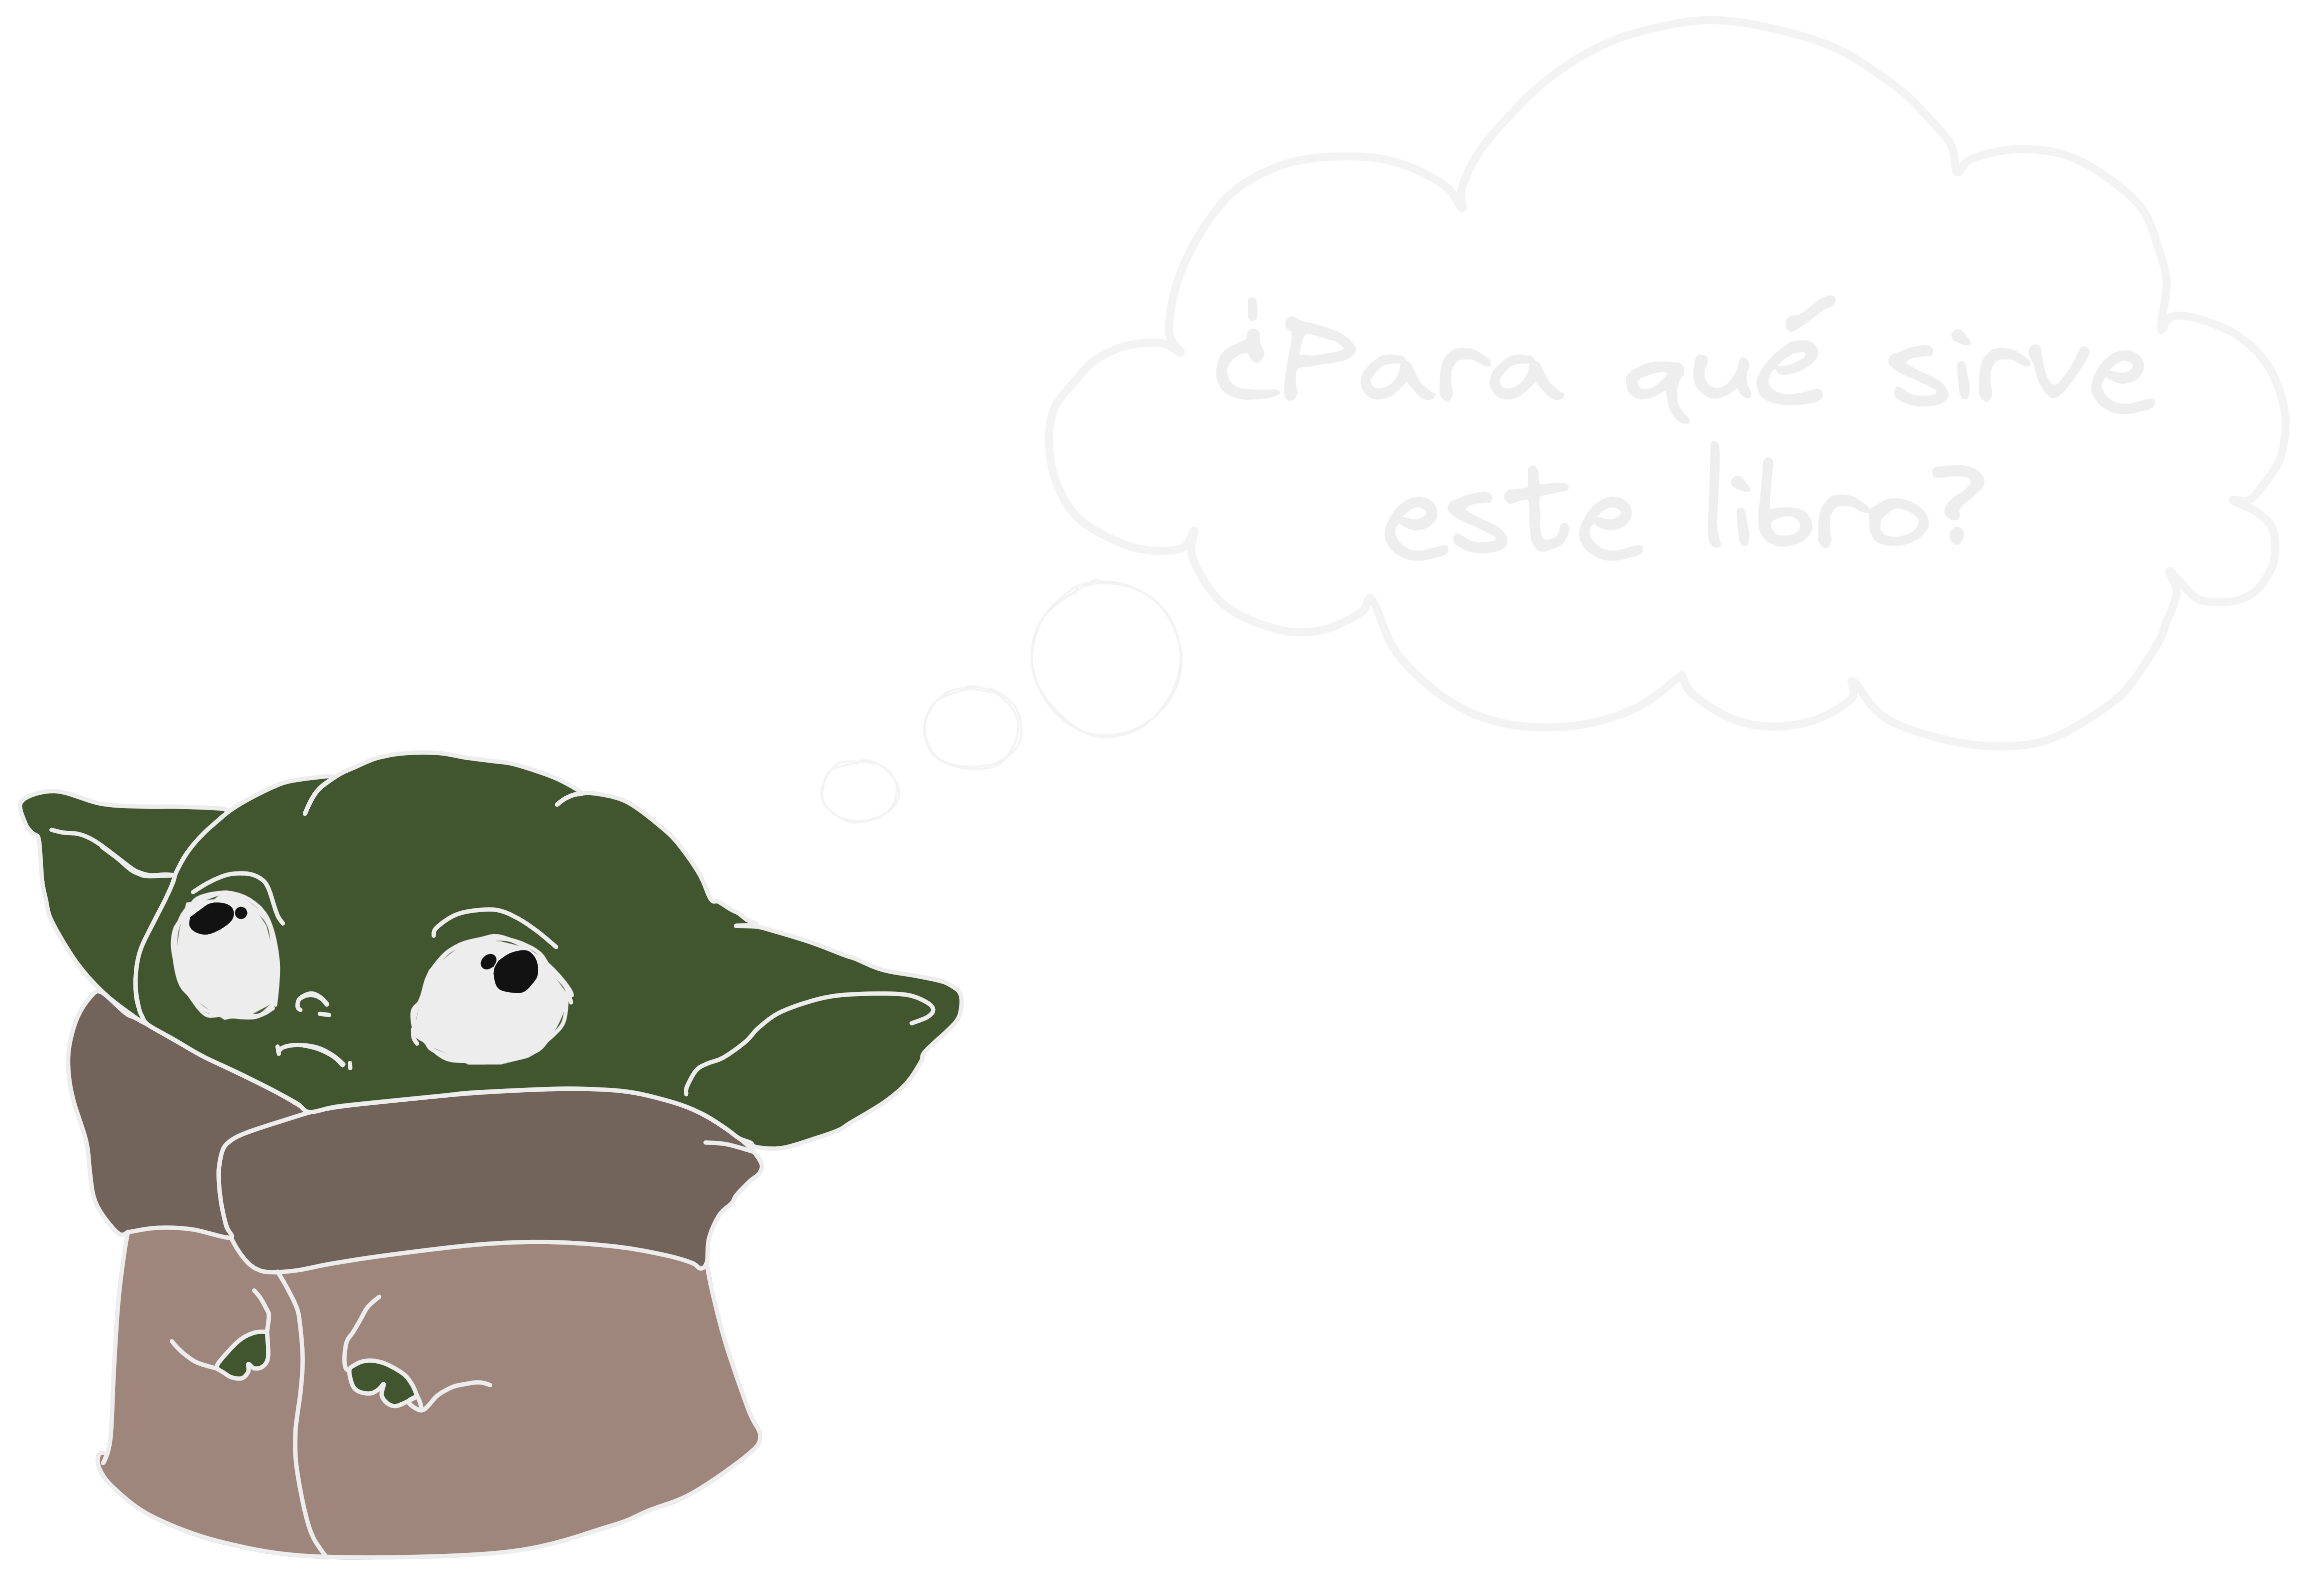
\includegraphics[width=2.08333in,height=\textheight]{images/para que sirve-2.png}

}

\end{figure}

Este curso está diseñado para principiantes y aquellos con poca o
ninguna experiencia en programación. No importa si eres un estudiante
curioso, un profesional que busca cambiar de carrera o simplemente
alguien que desea aprender a programar: este curso es para ti. Desde
adolescentes hasta adultos, todos son bienvenidos a participar y
explorar el emocionante mundo de la programación a través de Python.

\section{¿Cómo contribuir?}\label{cuxf3mo-contribuir}

\begin{figure}

{\centering \includegraphics[width=4.16667in,height=\textheight]{images/cómo contribuir.png}

}

\end{figure}

Valoramos tu participación en este curso. Si encuentras errores, deseas
sugerir mejoras o agregar contenido adicional, ¡nos encantaría
escucharte! Puedes contribuir a través de nuestra plataforma en línea,
donde puedes compartir tus comentarios y sugerencias. Juntos, podemos
mejorar continuamente este recurso educativo para beneficiar a la
comunidad de estudiantes y entusiastas de la programación.

Este libro ha sido creado con el objetivo de brindar acceso gratuito y
universal al conocimiento. Estará disponible en línea para que
cualquiera, sin importar su ubicación o circunstancias, pueda acceder y
aprender a su propio ritmo.

¡Esperamos que disfrutes este emocionante viaje de aprendizaje y
descubrimiento en el mundo de la programación con Python!

\part{Unidad 1: Introducción a Python}

\chapter{Introducción general a la
Programación}\label{introducciuxf3n-general-a-la-programaciuxf3n}

La programación es el proceso de crear secuencias de instrucciones que
le indican a una computadora cómo realizar una tarea específica.

Estas instrucciones se escriben en lenguajes de programación, que son
conjuntos de reglas y símbolos utilizados para comunicarse con la
máquina. La programación es una habilidad esencial en la era digital, ya
que se aplica en una amplia variedad de campos, desde desarrollo de
software y análisis de datos hasta diseño de juegos y automatización.

\section{Conceptos Clave}\label{conceptos-clave}

\subsection{Instrucciones}\label{instrucciones}

Son comandos específicos que le indican a la computadora qué hacer.
Pueden ser simples, como imprimir un mensaje en pantalla, o complejas,
como realizar cálculos matemáticos.

\subsection{Lenguajes de
Programación.}\label{lenguajes-de-programaciuxf3n.}

Son sistemas de comunicación entre humanos y máquinas. Cada lenguaje
tiene reglas sintácticas y semánticas que determinan cómo se escriben y
ejecutan las instrucciones.

\subsection{Algoritmos}\label{algoritmos}

Son conjuntos ordenados de instrucciones diseñados para resolver un
problema específico. Los algoritmos son la base de la programación y se
utilizan para desarrollar software eficiente.

\subsection{Depuración}\label{depuraciuxf3n}

\begin{figure}

{\centering 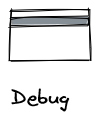
\includegraphics{unidades/unidad1/images/debug.png}

}

\end{figure}

Es el proceso de identificar y corregir errores en el código. Los
programadores pasan tiempo depurando para asegurarse de que sus
programas funcionen correctamente.

\section{Ejemplo:}\label{ejemplo}

\phantomsection\label{annotated-cell-1}%
\begin{Shaded}
\begin{Highlighting}[]
\BuiltInTok{print}\NormalTok{(}\StringTok{"Hola, bienvenido al mundo de la programación."}\NormalTok{)}\hspace*{\fill}\NormalTok{\circled{1}}
\end{Highlighting}
\end{Shaded}

\begin{description}
\tightlist
\item[\circled{1}]
Este es un ejemplo sencillo de un programa en Python que imprime un
mensaje en pantalla.
\end{description}

\section{Explicación}\label{explicaciuxf3n}

En Python, los comentarios comienzan con el símbolo \texttt{\#}. No
afectan la ejecución del programa, pero son útiles para documentar el
código.

La línea
\texttt{print("Hola,\ bienvenido\ al\ mundo\ de\ la\ programación.")} es
una instrucción de impresión. La función \texttt{print()} muestra el
texto entre paréntesis en la consola.

\begin{tcolorbox}[enhanced jigsaw, toptitle=1mm, toprule=.15mm, title=\textcolor{quarto-callout-tip-color}{\faLightbulb}\hspace{0.5em}{Tip}, colbacktitle=quarto-callout-tip-color!10!white, opacitybacktitle=0.6, titlerule=0mm, colback=white, left=2mm, bottomrule=.15mm, breakable, bottomtitle=1mm, rightrule=.15mm, colframe=quarto-callout-tip-color-frame, arc=.35mm, leftrule=.75mm, coltitle=black, opacityback=0]

\textbf{Actividad Práctica}

Escribe un programa que solicite al usuario su nombre y luego imprima un
mensaje de bienvenida personalizado.

\end{tcolorbox}

\section{Explicación de la
Actividad}\label{explicaciuxf3n-de-la-actividad}

El programa utilizará la función \texttt{input()} para recibir la
entrada del usuario. Luego, utilizará la entrada proporcionada para
imprimir un mensaje de bienvenida personalizado.

\chapter{Instalación de Python}\label{instalaciuxf3n-de-python}

La instalación de Python es el primer paso para comenzar a programar en
este lenguaje. Python es un lenguaje de programación versátil y
ampliamente utilizado, conocido por su sintaxis clara y legible. Aquí
aprenderemos cómo instalar Python en diferentes sistemas operativos.

\section{Conceptos Clave}\label{conceptos-clave-1}

\subsection{Python}\label{python}

\begin{figure}

{\centering 
\includegraphics[width=1.5625in,height=\textheight]{unidades/unidad1/images/python.png}

}

\end{figure}

Lenguaje de programación de alto nivel que se utiliza para desarrollar
aplicaciones web, científicas, de automatización y más.

\subsection{Interprete}\label{interprete}

\begin{figure}

{\centering 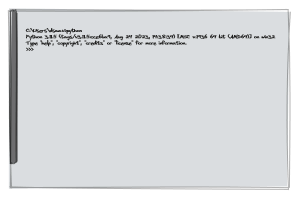
\includegraphics{unidades/unidad1/images/interprete.png}

}

\end{figure}

Python es un lenguaje interpretado, lo que significa que se ejecuta
línea por línea en tiempo real.

\subsection{IDE}\label{ide}

\begin{figure}

{\centering 
\includegraphics[width=1.5625in,height=\textheight]{unidades/unidad1/images/vscode.png}

}

\end{figure}

Los entornos de desarrollo integrados (IDE) como Visual Studio Code (VS
Code) o PyCharm brindan herramientas para escribir, depurar y ejecutar
código de manera más eficiente.

\section{Ejemplo}\label{ejemplo-1}

No se necesita código para esta lección, ya que se trata de
instrucciones para la instalación de Python en diferentes sistemas
operativos.

\section{Explicación}\label{explicaciuxf3n-1}

Para instalar Python en sistemas Windows, macOS y Linux, se pueden
seguir las instrucciones detalladas proporcionadas en el sitio web
oficial de Python
\href{https://www.python.org/downloads/}{www.python.org/downloads/}.

La instalación de Python generalmente incluye el intérprete de Python y
una serie de herramientas y bibliotecas estándar que hacen que sea fácil
comenzar a programar.

\begin{tcolorbox}[enhanced jigsaw, toptitle=1mm, toprule=.15mm, title=\textcolor{quarto-callout-tip-color}{\faLightbulb}\hspace{0.5em}{Actividad Práctica}, colbacktitle=quarto-callout-tip-color!10!white, opacitybacktitle=0.6, titlerule=0mm, colback=white, left=2mm, bottomrule=.15mm, breakable, bottomtitle=1mm, rightrule=.15mm, colframe=quarto-callout-tip-color-frame, arc=.35mm, leftrule=.75mm, coltitle=black, opacityback=0]

Instala Python en tu sistema operativo siguiendo las instrucciones del
sitio web oficial de Python. Luego, verifica que Python esté
correctamente instalado ejecutando el intérprete y escribiendo el
siguiente código:

\begin{Shaded}
\begin{Highlighting}[]
\BuiltInTok{print}\NormalTok{(}\StringTok{"Python se ha instalado correctamente."}\NormalTok{)}
\end{Highlighting}
\end{Shaded}

\end{tcolorbox}

\section{Explicación de la
Actividad}\label{explicaciuxf3n-de-la-actividad-1}

Esta actividad permite a los participantes aplicar lo aprendido
instalando Python en su propio sistema y ejecutando un programa sencillo
para confirmar que la instalación fue exitosa.

\chapter{Uso del REPL, PEP 8 y el Zen de
Python}\label{uso-del-repl-pep-8-y-el-zen-de-python}

\begin{figure}

{\centering 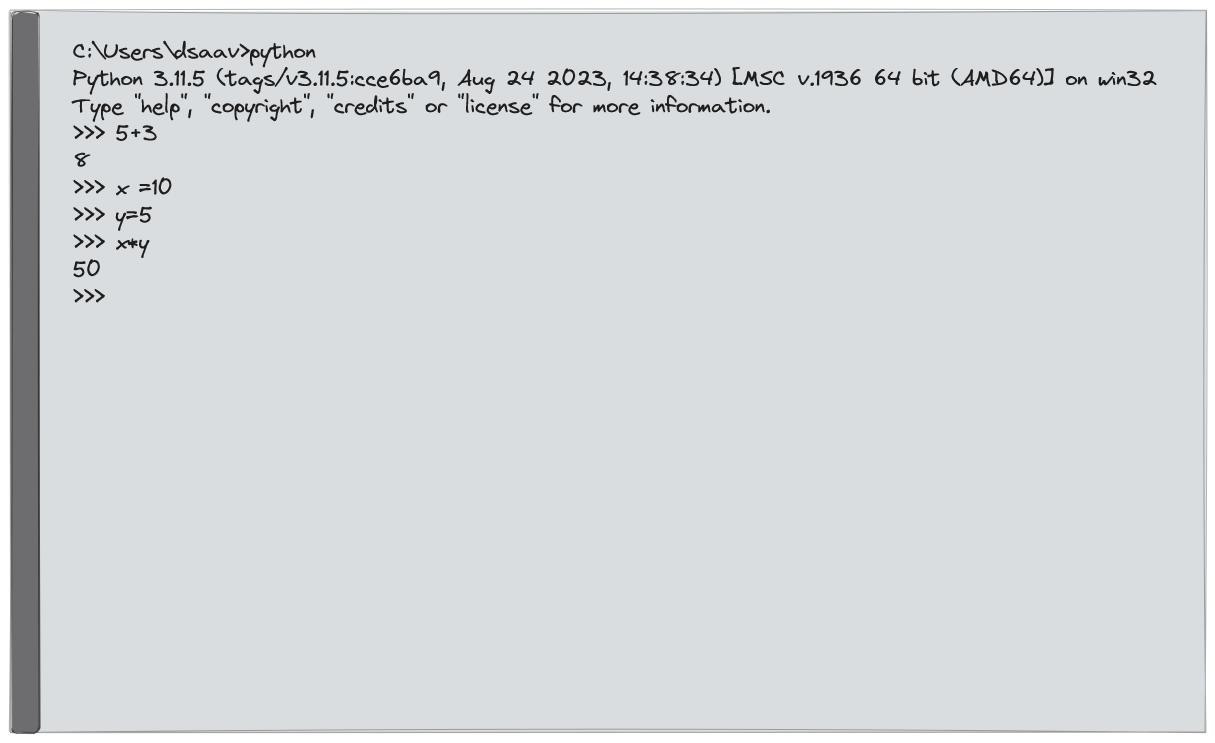
\includegraphics[width=4.16667in,height=\textheight]{unidades/unidad1/images/repl.png}

}

\end{figure}

\subsection{El REPL (Read-Eval-Print
Loop).}\label{el-repl-read-eval-print-loop.}

\textbf{Definición y Propósito del REPL.}

\begin{itemize}
\tightlist
\item
  El REPL (Read-Eval-Print Loop) es una herramienta interactiva que
  permite ejecutar código Python de forma inmediata y ver los resultados
  de las operaciones en tiempo real. Es una excelente manera de probar
  pequeños fragmentos de código, experimentar y depurar sin necesidad de
  escribir un programa completo.
\end{itemize}

\textbf{Uso Básico del REPL}

Para iniciar el REPL, simplemente abre una terminal o línea de comandos
y escribe python o python3 (dependiendo de tu instalación) seguido de
Enter. Esto te llevará al entorno interactivo de Python.

\subsection{Ejemplos de Interacción con el
REPL}\label{ejemplos-de-interacciuxf3n-con-el-repl}

\begin{Shaded}
\begin{Highlighting}[]
\CommentTok{\# Ejemplo 1: Realizar cálculos simples}
\OperatorTok{\textgreater{}\textgreater{}\textgreater{}} \DecValTok{5} \OperatorTok{+} \DecValTok{3}
\DecValTok{8}

\CommentTok{\# Ejemplo 2: Definir variables y realizar operaciones}
\OperatorTok{\textgreater{}\textgreater{}\textgreater{}}\NormalTok{ x }\OperatorTok{=} \DecValTok{10}
\OperatorTok{\textgreater{}\textgreater{}\textgreater{}}\NormalTok{ y }\OperatorTok{=} \DecValTok{5}
\OperatorTok{\textgreater{}\textgreater{}\textgreater{}}\NormalTok{ x }\OperatorTok{*}\NormalTok{ y}
\DecValTok{50}

\CommentTok{\# Ejemplo 3: Trabajar con cadenas de texto}
\OperatorTok{\textgreater{}\textgreater{}\textgreater{}}\NormalTok{ mensaje }\OperatorTok{=} \StringTok{"Hola, mundo!"}
\OperatorTok{\textgreater{}\textgreater{}\textgreater{}}\NormalTok{ mensaje.upper()}
\CommentTok{\textquotesingle{}HOLA, MUNDO!\textquotesingle{}}

\CommentTok{\# Ejemplo 4: Importar módulos y usar funciones}
\OperatorTok{\textgreater{}\textgreater{}\textgreater{}} \ImportTok{import}\NormalTok{ math}
\OperatorTok{\textgreater{}\textgreater{}\textgreater{}}\NormalTok{ math.sqrt(}\DecValTok{16}\NormalTok{)}
\FloatTok{4.0}
\end{Highlighting}
\end{Shaded}

\subsection{PEP 8: Guía de Estilo de
Python.}\label{pep-8-guuxeda-de-estilo-de-python.}

\begin{figure}

{\centering 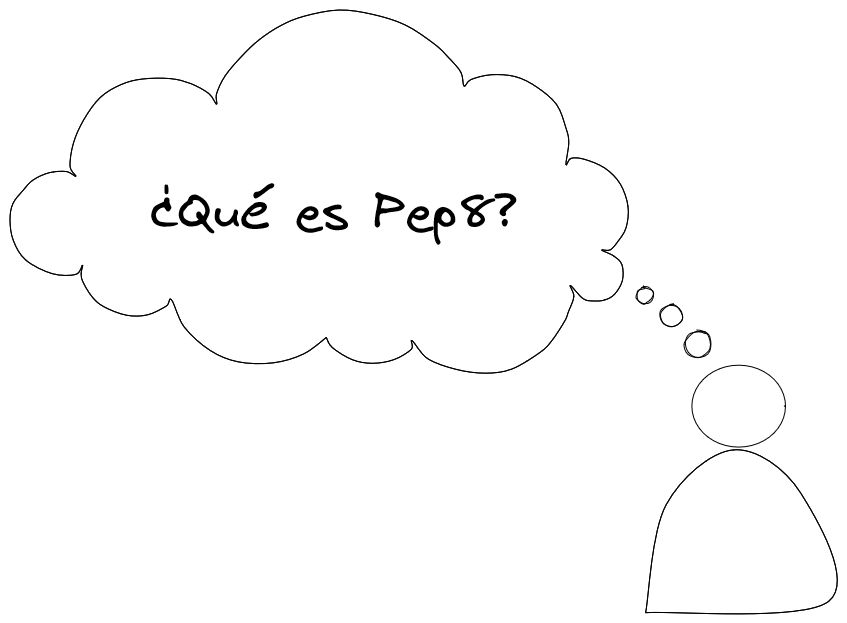
\includegraphics[width=2.08333in,height=\textheight]{unidades/unidad1/images/Que es pep8.png}

}

\end{figure}

\textbf{¿Qué es PEP 8 y Por Qué es Importante?}

PEP 8 (Python Enhancement Proposal 8) es una guía de estilo que
establece convenciones para escribir código Python legible y
consistente. La adopción de PEP 8 es importante porque facilita la
colaboración en proyectos, mejora la legibilidad del código y ayuda a
mantener una base de código ordenada y coherente.

\textbf{Convenciones de Nombres}

PEP 8 establece reglas para nombrar variables, funciones, clases y
módulos en Python. Algunas convenciones clave incluyen:

\begin{itemize}
\item
  Las variables y funciones deben usar minúsculas y palabras separadas
  por guiones bajos (snake\_case).
\item
  Las clases deben usar CamelCase (con la primera letra en mayúscula).
  Los módulos deben tener nombres cortos y en minúsculas.
\end{itemize}

\textbf{Reglas de Formato y Estilo}

PEP 8 también define reglas de formato, como el uso de espacios en lugar
de tabulaciones, la longitud máxima de línea y la organización de
importaciones.

\textbf{Herramientas para Verificar el Cumplimiento de PEP 8}

Existen herramientas como flake8 y complementos para editores de código
que pueden analizar el código en busca de posibles violaciones de PEP 8
y proporcionar sugerencias de corrección. 2.4.3. El Zen de Python

\subsection{Introducción al Zen de Python (PEP
20).}\label{introducciuxf3n-al-zen-de-python-pep-20.}

\begin{figure}

{\centering 
\includegraphics[width=2.08333in,height=\textheight]{unidades/unidad1/images/import this-2.png}

}

\end{figure}

El Zen de Python es un conjunto de principios y filosofía de diseño que
guían el desarrollo de Python. Estos principios se pueden acceder desde
el intérprete de Python utilizando el siguiente comando:

\begin{Shaded}
\begin{Highlighting}[]
\ImportTok{import}\NormalTok{ this}
\end{Highlighting}
\end{Shaded}

Los principios del Zen de Python proporcionan orientación sobre cómo
escribir código Python de manera clara y elegante.

\textbf{Principios y Filosofía de Diseño de Python}

Algunos de los principios más destacados del Zen de Python incluyen:

\begin{itemize}
\tightlist
\item
  \textbf{La legibilidad cuenta:} El código debe ser legible para los
  humanos, ya que se lee con más frecuencia de lo que se escribe.
\item
  \textbf{Explícito es mejor que implícito:} El código debe ser claro y
  no dejar lugar a ambigüedades.
\item
  \textbf{La simplicidad vence a la complejidad:} Debe preferirse la
  simplicidad en el diseño y la implementación.
\item
  \textbf{Los errores nunca deben pasar en silencio:} Los errores deben
  manejarse adecuadamente y, si es posible, informar de manera
  explícita.
\end{itemize}

\subsection{Ejercicios Prácticos}\label{ejercicios-pruxe1cticos}

\begin{itemize}
\tightlist
\item
  \textbf{Ejercicio 1:} Uso del REPL para Realizar Cálculos Simples
\end{itemize}

\begin{description}
\tightlist
\item[\circled{1}]
Abre el REPL de Python.
\end{description}

\begin{itemize}
\item
  \textbf{Ejercicio 2:} Verificación de Cumplimiento de PEP 8 en Código
  Python
\item
  Escribe un pequeño programa en Python que incluya variables, funciones
  y comentarios.
\item
  Utiliza la herramienta flake8 o un complemento de tu editor de código
  para verificar si tu código cumple con las reglas de PEP 8.
\item
  Corrige cualquier violación de PEP 8 y vuelve a verificar el código.
\item
  \textbf{Ejercicio 3:} Exploración y Reflexión sobre los Principios del
  Zen de Python
\item
  Ejecuta el comando import this en el REPL para acceder a los
  principios del Zen de Python.
\item
  Lee y reflexiona sobre cada uno de los principios.
\item
  Escribe un breve párrafo sobre cómo un principio específico del Zen de
  Python puede aplicarse al desarrollo de software.
\end{itemize}

\begin{tcolorbox}[enhanced jigsaw, toptitle=1mm, toprule=.15mm, title=\textcolor{quarto-callout-tip-color}{\faLightbulb}\hspace{0.5em}{Tip}, colbacktitle=quarto-callout-tip-color!10!white, opacitybacktitle=0.6, titlerule=0mm, colback=white, left=2mm, bottomrule=.15mm, breakable, bottomtitle=1mm, rightrule=.15mm, colframe=quarto-callout-tip-color-frame, arc=.35mm, leftrule=.75mm, coltitle=black, opacityback=0]

\textbf{Actividad Práctica}

\begin{itemize}
\item
  Desarrolla un pequeño programa Python que siga las pautas de PEP 8 y
  refleje los principios del Zen de Python en su diseño y estilo de
  codificación. Asegúrate de que el código sea legible y cumpla con las
  convenciones de nombres y formato de PEP 8.
\item
  Esta subunidad proporciona a los estudiantes una comprensión más
  profunda de las herramientas y las convenciones de estilo que se
  utilizan en la programación en Python. Además, les ayuda a reflexionar
  sobre la filosofía de diseño de Python y cómo aplicarla en la
  práctica.
\end{itemize}

\end{tcolorbox}

\subsection{Explicación}\label{explicaciuxf3n-2}

Esta actividad te invita a desarrollar un pequeño programa en Python que
siga las pautas de PEP 8 y refleje los principios del Zen de Python en
su diseño y estilo de codificación. La importancia de esta tarea radica
en aprender a escribir código que sea limpio, legible y siga las
convenciones de la comunidad de Python.

\begin{itemize}
\item
  \textbf{Cumplir con PEP 8}: PEP 8 es el estándar de estilo de código
  para Python, y seguirlo es una práctica recomendada en la comunidad de
  programadores. Tu programa debe seguir las convenciones de formato,
  nombres de variables, estructura de código, entre otros aspectos que
  se describen en PEP 8.
\item
  \textbf{Reflejar el Zen de Python}: El Zen de Python es una colección
  de principios filosóficos que guían el diseño del lenguaje Python.
  Algunos de estos principios incluyen la legibilidad del código, la
  simplicidad y la importancia de los casos especiales. Tu programa debe
  reflejar estos principios en su diseño y estilo de codificación.
\item
  \textbf{Legibilidad y Comentarios}: Asegúrate de que tu código sea
  legible para otras personas. Usa nombres de variables descriptivos,
  agrega comentarios explicativos cuando sea necesario y sigue las
  mejores prácticas para hacer que tu código sea fácil de entender.
\item
  \textbf{Aplicación Práctica}: Esta actividad te brinda la oportunidad
  de aplicar los conceptos de estilo de código y filosofía de diseño de
  Python en un proyecto real. Esto es importante ya que en la
  programación colaborativa, otros desarrolladores deben poder entender
  y trabajar con tu código de manera eficiente.
\end{itemize}

Al completar esta actividad, habrás mejorado tus habilidades en la
escritura de código Python de alta calidad y te habrás familiarizado con
las convenciones y filosofía de diseño de Python. Recuerda que escribir
código limpio es una habilidad esencial para cualquier programador.

\chapter{Entornos de Desarrollo}\label{entornos-de-desarrollo}

\part{Unidad 2: Introducción a la Programación con Python}

\chapter{Identación y Comentarios}\label{identaciuxf3n-y-comentarios}

\section{Identación}\label{identaciuxf3n}

\section{Conceptos Clave}\label{conceptos-clave-2}

\subsection{Identación}\label{identaciuxf3n-1}

\begin{itemize}
\tightlist
\item
  Espacios o tabulaciones al comienzo de una línea que indican la
  estructura del código.
\item
  \textbf{Bloques de Código:} Conjuntos de instrucciones que se agrupan
  juntas y se ejecutan en conjunto.
\item
  \textbf{PEP 8:} Guía de estilo para la escritura de código en Python
  que recomienda el uso de cuatro espacios para la identación.
\end{itemize}

\textbf{Ejemplo}:

\begin{Shaded}
\begin{Highlighting}[]
\CommentTok{\# Uso de la identación en un condicional}
\NormalTok{numero }\OperatorTok{=} \DecValTok{10}

\ControlFlowTok{if}\NormalTok{ numero }\OperatorTok{\textgreater{}} \DecValTok{5}\NormalTok{:}
    \BuiltInTok{print}\NormalTok{(}\StringTok{"El número es mayor que 5"}\NormalTok{)}
\ControlFlowTok{else}\NormalTok{:}
    \BuiltInTok{print}\NormalTok{(}\StringTok{"El número no es mayor que 5"}\NormalTok{)}
\end{Highlighting}
\end{Shaded}

\begin{tcolorbox}[enhanced jigsaw, toptitle=1mm, toprule=.15mm, title=\textcolor{quarto-callout-tip-color}{\faLightbulb}\hspace{0.5em}{Actividad Práctica}, colbacktitle=quarto-callout-tip-color!10!white, opacitybacktitle=0.6, titlerule=0mm, colback=white, left=2mm, bottomrule=.15mm, breakable, bottomtitle=1mm, rightrule=.15mm, colframe=quarto-callout-tip-color-frame, arc=.35mm, leftrule=.75mm, coltitle=black, opacityback=0]

\begin{enumerate}
\def\labelenumi{\arabic{enumi}.}
\tightlist
\item
  Escribe un programa que solicite al usuario su edad y muestre un
  mensaje según si es mayor de 18 años o no.
\end{enumerate}

\end{tcolorbox}

Posible solución

\textbf{Resumen}:

Esta actividad permite a los participantes comprender la importancia de
la identación en Python al trabajar con bloques de código como los
condicionales. Les ayuda a desarrollar el hábito de utilizar la
identación adecuada para mantener el código organizado y legible.

\begin{Shaded}
\begin{Highlighting}[]
\CommentTok{\# Programa que solicita la edad y muestra un mensaje}
\NormalTok{edad }\OperatorTok{=} \BuiltInTok{int}\NormalTok{(}\BuiltInTok{input}\NormalTok{(}\StringTok{"Ingrese su edad: "}\NormalTok{))}

\ControlFlowTok{if}\NormalTok{ edad }\OperatorTok{\textgreater{}} \DecValTok{18}\NormalTok{:}
    \BuiltInTok{print}\NormalTok{(}\StringTok{"Eres mayor de edad."}\NormalTok{)}
\ControlFlowTok{else}\NormalTok{:}
    \BuiltInTok{print}\NormalTok{(}\StringTok{"Eres menor de edad."}\NormalTok{)}
\end{Highlighting}
\end{Shaded}

\textbf{¿Qué hicimos?}

\begin{description}
\tightlist
\item[\circled{1}]
Se solicita la edad al usuario y se almacena en la variable edad.
\end{description}

\section{Comentarios}\label{comentarios}

\section{Conceptos Clave}\label{conceptos-clave-3}

\subsection{Comentarios}\label{comentarios-1}

\begin{itemize}
\tightlist
\item
  Son notas en el código que no se ejecutan y se utilizan para explicar
  el propósito y funcionamiento de partes del programa.
\item
  Comentarios de una línea: Se crean con el símbolo ``\#'' y abarcan una
  sola línea.
\item
  Comentarios de múltiples líneas: Se crean entre triple comillas
  (``\,``\,'' o '\,'\,') y pueden abarcar múltiples líneas.
\end{itemize}

\textbf{Ejemplo}:

\begin{Shaded}
\begin{Highlighting}[]
\CommentTok{\# Este es un comentario de una línea}

\CommentTok{"""}
\CommentTok{Este es un comentario}
\CommentTok{de múltiples líneas.}
\CommentTok{Puede abarcar varias líneas.}
\CommentTok{"""}

\NormalTok{numero }\OperatorTok{=} \DecValTok{42}  \CommentTok{\# Este comentario está después de una instrucción}
\end{Highlighting}
\end{Shaded}

\begin{tcolorbox}[enhanced jigsaw, toptitle=1mm, toprule=.15mm, title=\textcolor{quarto-callout-tip-color}{\faLightbulb}\hspace{0.5em}{Actividad Práctica}, colbacktitle=quarto-callout-tip-color!10!white, opacitybacktitle=0.6, titlerule=0mm, colback=white, left=2mm, bottomrule=.15mm, breakable, bottomtitle=1mm, rightrule=.15mm, colframe=quarto-callout-tip-color-frame, arc=.35mm, leftrule=.75mm, coltitle=black, opacityback=0]

Escribe un programa que realice una tarea sencilla y agrega comentarios
para explicar lo que hace cada parte. Escribe un comentario de múltiples
líneas que explique el propósito general de tu programa.

\end{tcolorbox}

Posible solución

\begin{Shaded}
\begin{Highlighting}[]
\CommentTok{\# Este programa calcula el área de un triángulo}
\CommentTok{\# solicitando la base y la altura al usuario.}

\CommentTok{\# Solicitar la base y almacenarla en la variable \textquotesingle{}base\textquotesingle{}}
\NormalTok{base }\OperatorTok{=} \BuiltInTok{float}\NormalTok{(}\BuiltInTok{input}\NormalTok{(}\StringTok{"Ingrese la base del triángulo: "}\NormalTok{))}

\CommentTok{\# Solicitar la altura y almacenarla en la variable \textquotesingle{}altura\textquotesingle{}}
\NormalTok{altura }\OperatorTok{=} \BuiltInTok{float}\NormalTok{(}\BuiltInTok{input}\NormalTok{(}\StringTok{"Ingrese la altura del triángulo: "}\NormalTok{))}

\CommentTok{\# Calcular el área del triángulo}
\NormalTok{area }\OperatorTok{=} \FloatTok{0.5} \OperatorTok{*}\NormalTok{ base }\OperatorTok{*}\NormalTok{ altura}

\CommentTok{\# Mostrar el resultado}
\BuiltInTok{print}\NormalTok{(}\SpecialStringTok{f"El área del triángulo es: }\SpecialCharTok{\{}\NormalTok{area}\SpecialCharTok{\}}\SpecialStringTok{"}\NormalTok{)}
\end{Highlighting}
\end{Shaded}

\section{¿Qué aprendimos?}\label{quuxe9-aprendimos}

En este tema, aprendimos la importancia de la identación en Python para
estructurar nuestro código correctamente. La identación nos permite
definir bloques de código, como en los condicionales, de manera clara y
legible.

También aprendimos cómo agregar comentarios en Python para documentar
nuestro código. Los comentarios son esenciales para explicar el
propósito y el funcionamiento de las partes del programa y facilitan la
colaboración entre programadores.

\chapter{Variables y Variables
Múltiples}\label{variables-y-variables-muxfaltiples}

\section{Variables}\label{variables}

Las variables son fundamentales en la programación ya que permiten
almacenar y manipular datos. Aprenderemos cómo declarar y utilizar
variables en Python.

\subsection{Conceptos Clave}\label{conceptos-clave-4}

\textbf{Variables}

\begin{itemize}
\tightlist
\item
  Nombres que representan ubicaciones de memoria donde se almacenan
  datos.
\end{itemize}

\textbf{Declaración de Variables}

\begin{itemize}
\tightlist
\item
  Asignación de un valor a un nombre utilizando el operador ``=''.
\item
  Convenciones de Nombres: Siguen reglas para ser descriptivos y seguir
  una estructura (por ejemplo, letras minúsculas y guiones bajos para
  espacios).
\end{itemize}

\textbf{Ejemplo}:

\begin{Shaded}
\begin{Highlighting}[]
\NormalTok{nombre }\OperatorTok{=} \StringTok{"Ana"}
\NormalTok{edad }\OperatorTok{=} \DecValTok{30}
\NormalTok{saldo\_bancario }\OperatorTok{=} \FloatTok{1500.75}
\NormalTok{es\_mayor\_de\_edad }\OperatorTok{=} \VariableTok{True}
\end{Highlighting}
\end{Shaded}

En este ejemplo, se declaran variables para almacenar el nombre de una
persona, su edad, su saldo bancario y un valor booleano que indica si es
mayor de edad.

Los nombres de variables son descriptivos y siguen la convención de
nombres recomendada (letras minúsculas y guiones bajos para espacios).

\begin{tcolorbox}[enhanced jigsaw, toptitle=1mm, toprule=.15mm, title=\textcolor{quarto-callout-tip-color}{\faLightbulb}\hspace{0.5em}{Actividad Práctica}, colbacktitle=quarto-callout-tip-color!10!white, opacitybacktitle=0.6, titlerule=0mm, colback=white, left=2mm, bottomrule=.15mm, breakable, bottomtitle=1mm, rightrule=.15mm, colframe=quarto-callout-tip-color-frame, arc=.35mm, leftrule=.75mm, coltitle=black, opacityback=0]

\begin{enumerate}
\def\labelenumi{\arabic{enumi}.}
\item
  Crea variables para almacenar información personal, como tu ciudad, tu
  edad y tu ocupación.
\item
  Declara variables para almacenar cantidades numéricas, como el precio
  de un producto y la cantidad de unidades disponibles.
\end{enumerate}

\end{tcolorbox}

\section{Explicación de la
Actividad.}\label{explicaciuxf3n-de-la-actividad.}

Esta actividad permite a los participantes practicar la declaración de
variables en Python y aplicar el concepto de convenciones de nombres.
Les ayuda a comprender cómo almacenar y acceder a datos utilizando
variables descriptivas y significativas. Múltiples Variables

En Python, es posible asignar valores a múltiples variables en una sola
línea. Aprenderemos cómo declarar y utilizar múltiples variables de
manera eficiente.

\subsection{Conceptos Clave}\label{conceptos-clave-5}

\textbf{Asignación Múltiple}

\begin{itemize}
\tightlist
\item
  Permite asignar valores a varias variables en una línea.
\end{itemize}

\textbf{Desempaquetado de Valores}

\begin{itemize}
\tightlist
\item
  Se pueden asignar valores de una lista o tupla a múltiples variables
  en una sola operación.
\end{itemize}

\textbf{Intercambio de Valores}

\begin{itemize}
\tightlist
\item
  Se pueden intercambiar los valores de dos variables utilizando
  asignación múltiple.
\end{itemize}

\textbf{Ejemplo}:

\begin{Shaded}
\begin{Highlighting}[]
\NormalTok{nombre, edad, altura }\OperatorTok{=} \StringTok{"María"}\NormalTok{, }\DecValTok{28}\NormalTok{, }\FloatTok{1.65}
\NormalTok{productos }\OperatorTok{=}\NormalTok{ (}\StringTok{"Manzanas"}\NormalTok{, }\StringTok{"Peras"}\NormalTok{, }\StringTok{"Uvas"}\NormalTok{)}
\NormalTok{producto1, producto2, producto3 }\OperatorTok{=}\NormalTok{ productos}
\end{Highlighting}
\end{Shaded}

\subsection{Explicación:}\label{explicaciuxf3n-3}

\begin{itemize}
\item
  En el primer ejemplo, se utilizó la asignación múltiple para declarar
  tres variables en una sola línea.
\item
  En el segundo ejemplo, se desempaquetaron los valores de una tupla en
  variables individuales.
\end{itemize}

\begin{tcolorbox}[enhanced jigsaw, toptitle=1mm, toprule=.15mm, title=\textcolor{quarto-callout-tip-color}{\faLightbulb}\hspace{0.5em}{Actividad Práctica}, colbacktitle=quarto-callout-tip-color!10!white, opacitybacktitle=0.6, titlerule=0mm, colback=white, left=2mm, bottomrule=.15mm, breakable, bottomtitle=1mm, rightrule=.15mm, colframe=quarto-callout-tip-color-frame, arc=.35mm, leftrule=.75mm, coltitle=black, opacityback=0]

\begin{enumerate}
\def\labelenumi{\arabic{enumi}.}
\item
  Crea una lista con los nombres de tus tres colores favoritos.
\item
  Utiliza la asignación múltiple para asignar los valores de la lista a
  tres variables individuales.
\end{enumerate}

\end{tcolorbox}

\subsection{Explicación de la
Actividad}\label{explicaciuxf3n-de-la-actividad-2}

Esta actividad permite a los participantes practicar la asignación
múltiple y el desempaquetado de valores. Les ayuda a comprender cómo
trabajar eficientemente con múltiples variables y cómo aprovechar estas
técnicas para simplificar el código.

\chapter{Concatenación}\label{concatenaciuxf3n}

\section{Conceptos Clave}\label{conceptos-clave-6}

\textbf{Concatenación}: La concatenación es la unión de cadenas de
texto. Aprenderemos cómo combinar cadenas de texto en Python para crear
mensajes más complejos.

\textbf{Operador +}: Se utiliza para concatenar cadenas de texto.

\textbf{Conversión a Cadena}: Es necesario convertir valores no string a
cadenas antes de concatenarlos.

\section{Ejemplo}\label{ejemplo-2}

\begin{Shaded}
\begin{Highlighting}[]
\NormalTok{nombre }\OperatorTok{=} \StringTok{"Luisa"}
\NormalTok{mensaje }\OperatorTok{=} \StringTok{"Hola, "} \OperatorTok{+}\NormalTok{ nombre }\OperatorTok{+} \StringTok{". ¿Cómo estás?"}
\NormalTok{edad }\OperatorTok{=} \DecValTok{25}
\NormalTok{mensaje\_edad }\OperatorTok{=} \StringTok{"Tienes "} \OperatorTok{+} \BuiltInTok{str}\NormalTok{(edad) }\OperatorTok{+} \StringTok{" años."}
\end{Highlighting}
\end{Shaded}

\subsection{Explicación:}\label{explicaciuxf3n-4}

En este ejemplo, se utilizó el operador ``+'' para concatenar cadenas de
texto. La variable ``edad'' se convirtió a una cadena utilizando la
función ``str()'' antes de concatenarla.

\begin{tcolorbox}[enhanced jigsaw, toptitle=1mm, toprule=.15mm, title=\textcolor{quarto-callout-tip-color}{\faLightbulb}\hspace{0.5em}{Actividad Práctica}, colbacktitle=quarto-callout-tip-color!10!white, opacitybacktitle=0.6, titlerule=0mm, colback=white, left=2mm, bottomrule=.15mm, breakable, bottomtitle=1mm, rightrule=.15mm, colframe=quarto-callout-tip-color-frame, arc=.35mm, leftrule=.75mm, coltitle=black, opacityback=0]

\begin{itemize}
\tightlist
\item
  Crea una variable con tu comida favorita.
\item
  Utiliza la concatenación para crear un mensaje que incluya tu comida
  favorita.
\end{itemize}

\end{tcolorbox}

\subsection{Explicación de la
Actividad:}\label{explicaciuxf3n-de-la-actividad-3}

Esta actividad permite a los participantes practicar la concatenación de
cadenas de texto y comprender cómo construir mensajes más complejos
utilizando variables y texto. Les ayuda a mejorar su capacidad para
crear mensajes personalizados en sus programas.

\part{Unidad 3: Tipos de Datos}

\chapter{String y Números}\label{string-y-nuxfameros}

\begin{figure}

{\centering 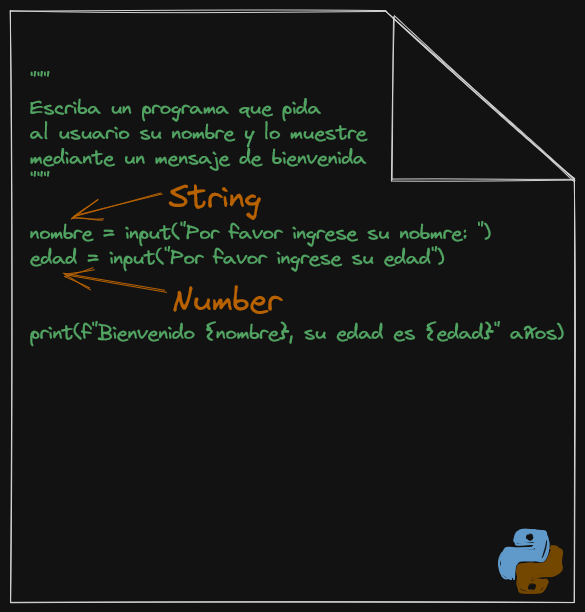
\includegraphics[width=4.16667in,height=\textheight]{unidades/unidad3/images/stringAndNumber.png}

}

\end{figure}

\section{Conceptos Clave}\label{conceptos-clave-7}

\textbf{String}

\begin{figure}

{\centering 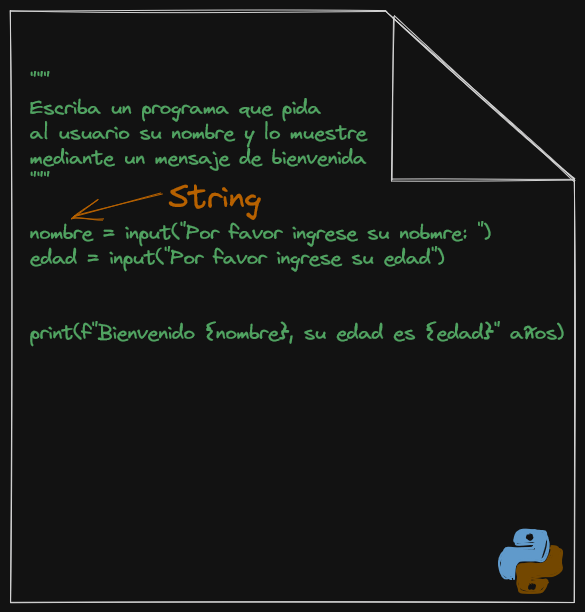
\includegraphics[width=4.16667in,height=\textheight]{unidades/unidad3/images/string-4.png}

}

\end{figure}

Un string es una secuencia de caracteres alfanuméricos. Se pueden
definir utilizando comillas simples o dobles.

\textbf{Números Enteros (int)}

\begin{figure}

{\centering 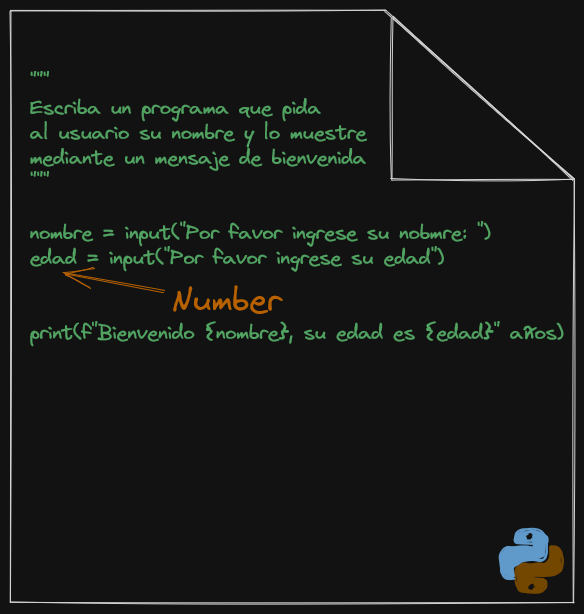
\includegraphics[width=4.16667in,height=\textheight]{unidades/unidad3/images/number.png}

}

\end{figure}

Los números enteros representan valores numéricos enteros, ya sean
positivos o negativos.

\textbf{Números de Punto Flotante (float)}

\begin{figure}

{\centering 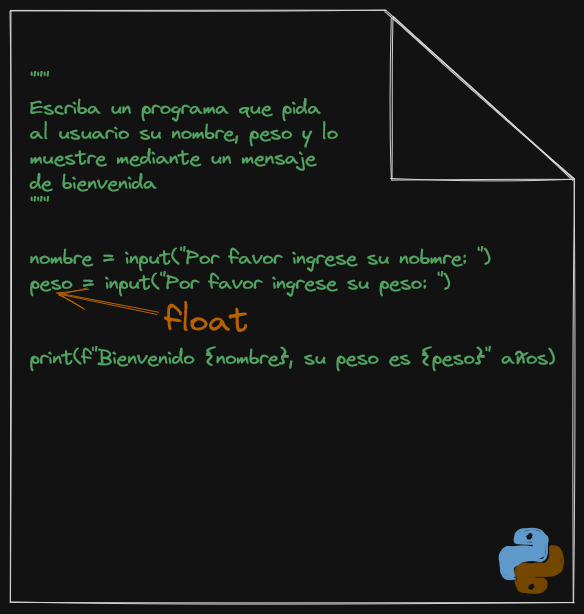
\includegraphics[width=4.16667in,height=\textheight]{unidades/unidad3/images/float.png}

}

\end{figure}

Los números de punto flotante representan valores numéricos con
decimales.

\section{Ejemplo}\label{ejemplo-3}

\begin{Shaded}
\begin{Highlighting}[]
\CommentTok{\# Strings}
\NormalTok{mensaje }\OperatorTok{=} \StringTok{"Hola, bienvenido al curso de Python."}
\NormalTok{nombre }\OperatorTok{=} \StringTok{\textquotesingle{}María\textquotesingle{}}

\CommentTok{\# Números}
\NormalTok{edad }\OperatorTok{=} \DecValTok{25}
\NormalTok{saldo }\OperatorTok{=} \FloatTok{1500.75}
\end{Highlighting}
\end{Shaded}

\subsection{Explicación:}\label{explicaciuxf3n-5}

En este ejemplo, se crean variables que almacenan strings y números. Los
strings se definen utilizando comillas simples o dobles, y los números
enteros y de punto flotante se asignan directamente a variables.

\begin{tcolorbox}[enhanced jigsaw, toptitle=1mm, toprule=.15mm, title=\textcolor{quarto-callout-tip-color}{\faLightbulb}\hspace{0.5em}{Actividad Práctica}, colbacktitle=quarto-callout-tip-color!10!white, opacitybacktitle=0.6, titlerule=0mm, colback=white, left=2mm, bottomrule=.15mm, breakable, bottomtitle=1mm, rightrule=.15mm, colframe=quarto-callout-tip-color-frame, arc=.35mm, leftrule=.75mm, coltitle=black, opacityback=0]

\begin{enumerate}
\def\labelenumi{\arabic{enumi}.}
\tightlist
\item
  Crea una variable con el título de tu canción favorita.
\item
  Asigna tu edad a una variable y tu altura a otra variable.
\item
  Combina las variables para crear un mensaje personalizado.
\end{enumerate}

\end{tcolorbox}

\subsection{Explicación:}\label{explicaciuxf3n-6}

Esta actividad permite a los participantes practicar la creación de
strings y trabajar con números enteros y de punto flotante. Les ayuda a
comprender cómo almacenar y manipular diferentes tipos de datos en
Python.

\section{¿Qué Aprendimos?}\label{quuxe9-aprendimos-1}

En esta lección, aprendimos sobre los dos tipos de datos fundamentales
en Python: strings y números. Aprendimos cómo crear y trabajar con
strings utilizando comillas simples o dobles. También exploramos dos
tipos numéricos clave: números enteros (int) y números de punto flotante
(float). Estos conceptos son esenciales para manejar información en
Python y forman la base de muchos programas y aplicaciones.

\chapter{Listas y Tuplas}\label{listas-y-tuplas}

\begin{figure}

{\centering 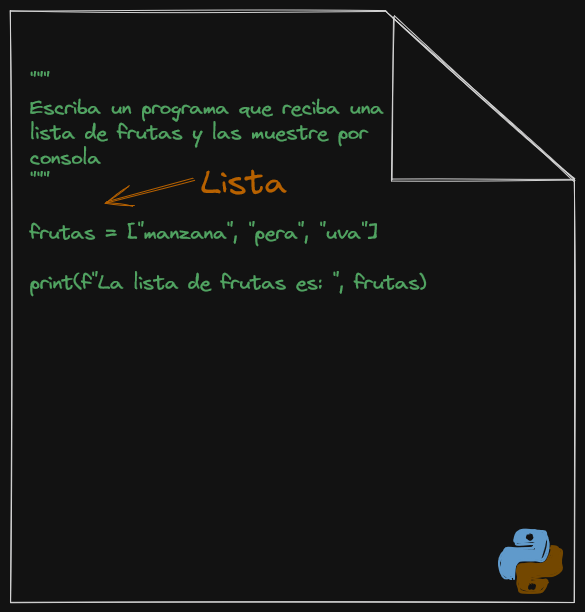
\includegraphics[width=4.16667in,height=\textheight]{unidades/unidad3/images/list.png}

}

\end{figure}

\section{Conceptos Clave}\label{conceptos-clave-8}

\subsection{Listas}\label{listas}

\begin{figure}

{\centering 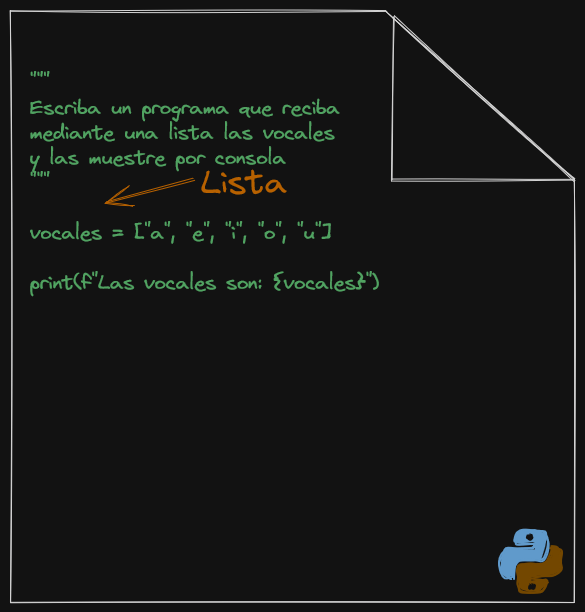
\includegraphics[width=4.16667in,height=\textheight]{unidades/unidad3/images/vocales.png}

}

\end{figure}

Las listas son secuencias ordenadas de elementos que pueden ser de
diferentes tipos. Permiten almacenar varios elementos en una sola
variable.

\subsection{Tuplas}\label{tuplas}

\begin{figure}

{\centering 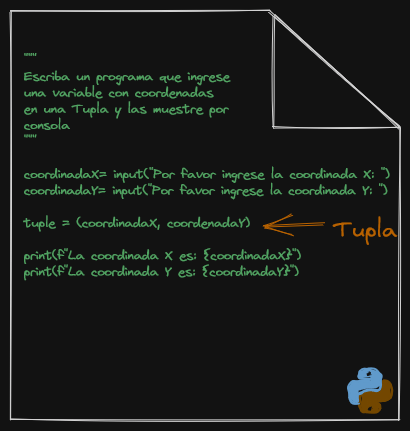
\includegraphics[width=4.16667in,height=\textheight]{unidades/unidad3/images/tuple.png}

}

\end{figure}

Las tuplas son similares a las listas, pero son inmutables, lo que
significa que no se pueden modificar después de ser creadas.

\section{Ejemplo}\label{ejemplo-4}

\begin{Shaded}
\begin{Highlighting}[]
\CommentTok{\# Listas}
\NormalTok{frutas }\OperatorTok{=}\NormalTok{ [}\StringTok{"manzana"}\NormalTok{, }\StringTok{"banana"}\NormalTok{, }\StringTok{"naranja"}\NormalTok{, }\StringTok{"uva"}\NormalTok{]}
\NormalTok{primer\_fruta }\OperatorTok{=}\NormalTok{ frutas[}\DecValTok{0}\NormalTok{]}
\NormalTok{segunda\_fruta }\OperatorTok{=}\NormalTok{ frutas[}\DecValTok{1}\NormalTok{]}

\CommentTok{\# Tuplas}
\NormalTok{coordenadas }\OperatorTok{=}\NormalTok{ (}\DecValTok{3}\NormalTok{, }\DecValTok{5}\NormalTok{)}
\NormalTok{x }\OperatorTok{=}\NormalTok{ coordenadas[}\DecValTok{0}\NormalTok{]}
\NormalTok{y }\OperatorTok{=}\NormalTok{ coordenadas[}\DecValTok{1}\NormalTok{]}
\end{Highlighting}
\end{Shaded}

\subsection{Explicación:}\label{explicaciuxf3n-7}

En este ejemplo, se crea una lista de frutas y una tupla de coordenadas.
Se accede a elementos individuales de la lista y la tupla utilizando
índices.

Los índices comienzan desde 0, por lo que la primera fruta tiene el
índice 0.

\begin{tcolorbox}[enhanced jigsaw, toptitle=1mm, toprule=.15mm, title=\textcolor{quarto-callout-tip-color}{\faLightbulb}\hspace{0.5em}{Actividad Práctica (Listas):}, colbacktitle=quarto-callout-tip-color!10!white, opacitybacktitle=0.6, titlerule=0mm, colback=white, left=2mm, bottomrule=.15mm, breakable, bottomtitle=1mm, rightrule=.15mm, colframe=quarto-callout-tip-color-frame, arc=.35mm, leftrule=.75mm, coltitle=black, opacityback=0]

\begin{enumerate}
\def\labelenumi{\arabic{enumi}.}
\tightlist
\item
  Crea una lista con los nombres de tus tres películas favoritas.
\item
  Accede al segundo elemento de la lista e imprímelo en la consola.
\end{enumerate}

\end{tcolorbox}

\subsection{Explicación:}\label{explicaciuxf3n-8}

Esta actividad permite a los participantes practicar la creación de
listas y el acceso a elementos utilizando índices. Les ayuda a
comprender cómo organizar y acceder a múltiples elementos en una sola
variable.

\begin{tcolorbox}[enhanced jigsaw, toptitle=1mm, toprule=.15mm, title=\textcolor{quarto-callout-tip-color}{\faLightbulb}\hspace{0.5em}{Actividad Práctica (Tuplas):}, colbacktitle=quarto-callout-tip-color!10!white, opacitybacktitle=0.6, titlerule=0mm, colback=white, left=2mm, bottomrule=.15mm, breakable, bottomtitle=1mm, rightrule=.15mm, colframe=quarto-callout-tip-color-frame, arc=.35mm, leftrule=.75mm, coltitle=black, opacityback=0]

\begin{enumerate}
\def\labelenumi{\arabic{enumi}.}
\tightlist
\item
  Crea una tupla con las estaciones del año.
\item
  Intenta modificar un elemento de la tupla y observa el error que se
  produce.
\end{enumerate}

\end{tcolorbox}

\subsection{Explicación:}\label{explicaciuxf3n-9}

Esta actividad permite a los participantes practicar la creación de
tuplas y comprender la diferencia entre listas y tuplas en términos de
inmutabilidad. Les ayuda a comprender cómo utilizar tuplas cuando
necesitan almacenar datos que no deben cambiar.

\section{¿Qué Aprendimos?}\label{quuxe9-aprendimos-2}

En esta lección, aprendimos sobre dos tipos de estructuras de datos en
Python: listas y tuplas.

\textbf{Listas}: Son secuencias ordenadas de elementos que pueden
modificarse. Se accede a los elementos utilizando índices.

\textbf{Tuplas}: Son similares a las listas, pero son inmutables, lo que
significa que no pueden modificarse después de su creación. También se
accede a los elementos utilizando índices.

Estas estructuras nos permiten almacenar y organizar datos de manera
eficiente en Python, y la elección entre listas y tuplas depende de si
necesitamos datos modificables o inmutables en nuestros programas.

\chapter{Diccionarios y Booleanos}\label{diccionarios-y-booleanos}

\section{Diccionarios}\label{diccionarios}

\begin{figure}

{\centering 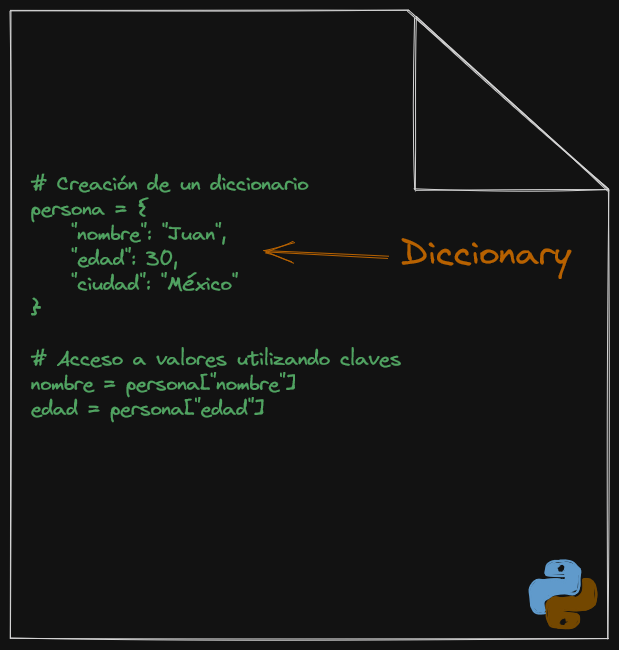
\includegraphics[width=4.16667in,height=\textheight]{unidades/unidad3/images/diccionary.png}

}

\end{figure}

\subsection{Conceptos Clave}\label{conceptos-clave-9}

\subsubsection{Diccionarios}\label{diccionarios-1}

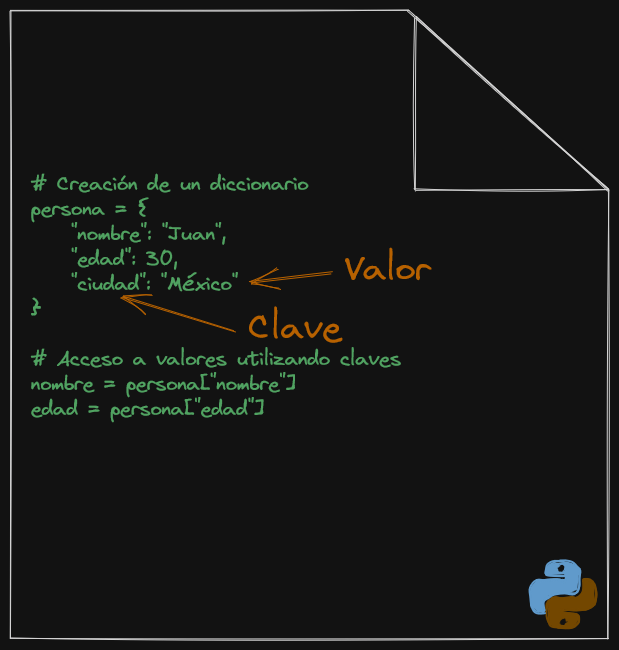
\includegraphics[width=4.16667in,height=\textheight]{unidades/unidad3/images/diccionary001.png}

Los diccionarios son estructuras de datos que almacenan pares
clave-valor.

\subsubsection{Claves}\label{claves}

Son los nombres o etiquetas utilizados para acceder a los valores en el
diccionario.

\subsubsection{Valores}\label{valores}

Son los datos asociados a cada clave en el diccionario.

\subsection{Ejemplo}\label{ejemplo-5}

\begin{Shaded}
\begin{Highlighting}[]
\CommentTok{\# Creación de un diccionario}
\NormalTok{persona }\OperatorTok{=}\NormalTok{ \{}
    \StringTok{"nombre"}\NormalTok{: }\StringTok{"Juan"}\NormalTok{,}
    \StringTok{"edad"}\NormalTok{: }\DecValTok{30}\NormalTok{,}
    \StringTok{"ciudad"}\NormalTok{: }\StringTok{"México"}
\NormalTok{\}}

\CommentTok{\# Acceso a valores utilizando claves}
\NormalTok{nombre }\OperatorTok{=}\NormalTok{ persona[}\StringTok{"nombre"}\NormalTok{]}
\NormalTok{edad }\OperatorTok{=}\NormalTok{ persona[}\StringTok{"edad"}\NormalTok{]}
\end{Highlighting}
\end{Shaded}

\subsection{Explicación:}\label{explicaciuxf3n-10}

En este ejemplo, se crea un diccionario que almacena información de una
persona, como nombre, edad y ciudad.

Se accede a los valores del diccionario utilizando las claves
correspondientes.

\begin{tcolorbox}[enhanced jigsaw, toptitle=1mm, toprule=.15mm, title=\textcolor{quarto-callout-tip-color}{\faLightbulb}\hspace{0.5em}{Actividad Práctica}, colbacktitle=quarto-callout-tip-color!10!white, opacitybacktitle=0.6, titlerule=0mm, colback=white, left=2mm, bottomrule=.15mm, breakable, bottomtitle=1mm, rightrule=.15mm, colframe=quarto-callout-tip-color-frame, arc=.35mm, leftrule=.75mm, coltitle=black, opacityback=0]

\begin{enumerate}
\def\labelenumi{\arabic{enumi}.}
\tightlist
\item
  Crea un diccionario que almacene información de tus libros favoritos,
  incluyendo título y autor.
\item
  Accede a los valores del diccionario utilizando las claves y muestra
  la información en la consola.
\end{enumerate}

\end{tcolorbox}

\subsection{Explicación:}\label{explicaciuxf3n-11}

Esta actividad permite a los participantes practicar la creación de
diccionarios y acceder a los valores utilizando las claves. Les ayuda a
comprender cómo organizar datos en pares clave-valor y cómo acceder a la
información de manera eficiente.

\section{Booleanos}\label{booleanos}

\section{Conceptos Clave}\label{conceptos-clave-10}

\textbf{Booleanos}

\begin{itemize}
\tightlist
\item
  Tipo de dato que representa valores de verdad (True o False).
\end{itemize}

\textbf{Expresiones Lógicas}: Combinaciones de valores booleanos
utilizando operadores lógicos como and, or y not. Ejemplo

\begin{Shaded}
\begin{Highlighting}[]
\CommentTok{\# Variables booleanas}
\NormalTok{es\_mayor\_de\_edad }\OperatorTok{=} \VariableTok{True}
\NormalTok{tiene\_tarjeta }\OperatorTok{=} \VariableTok{False}

\CommentTok{\# Expresiones lógicas}
\NormalTok{puede\_ingresar }\OperatorTok{=}\NormalTok{ es\_mayor\_de\_edad }\KeywordTok{and}\NormalTok{ tiene\_tarjeta}
\end{Highlighting}
\end{Shaded}

\subsection{Explicación:}\label{explicaciuxf3n-12}

En este ejemplo, se utilizan variables booleanas para representar si
alguien es mayor de edad y si tiene una tarjeta.

Se utiliza una expresión lógica para evaluar si alguien puede ingresar
basado en ambas condiciones.

\begin{tcolorbox}[enhanced jigsaw, toptitle=1mm, toprule=.15mm, title=\textcolor{quarto-callout-tip-color}{\faLightbulb}\hspace{0.5em}{Actividad Práctica}, colbacktitle=quarto-callout-tip-color!10!white, opacitybacktitle=0.6, titlerule=0mm, colback=white, left=2mm, bottomrule=.15mm, breakable, bottomtitle=1mm, rightrule=.15mm, colframe=quarto-callout-tip-color-frame, arc=.35mm, leftrule=.75mm, coltitle=black, opacityback=0]

\begin{enumerate}
\def\labelenumi{\arabic{enumi}.}
\tightlist
\item
  Crea variables booleanas que representen si tienes una mascota y si te
  gusta el deporte.
\item
  Utiliza expresiones lógicas para determinar si puedes llevar a tu
  mascota a un lugar que requiere tu atención durante un partido de tu
  deporte favorito.
\end{enumerate}

\end{tcolorbox}

\subsection{Explicación:}\label{explicaciuxf3n-13}

Esta actividad permite a los participantes practicar el uso de variables
booleanas y expresiones lógicas para tomar decisiones basadas en
condiciones booleanas. Les ayuda a comprender cómo trabajar con valores
de verdad y cómo utilizarlos para evaluar situaciones en el código.

\chapter{Range}\label{range}

\begin{figure}

{\centering 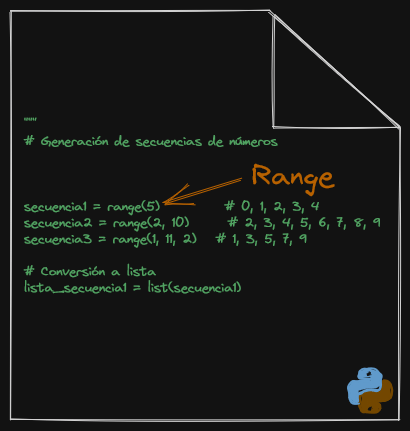
\includegraphics[width=4.16667in,height=\textheight]{unidades/unidad3/images/range.png}

}

\end{figure}

\section{Conceptos Clave}\label{conceptos-clave-11}

\subsection{range}\label{range-1}

\begin{itemize}
\tightlist
\item
  Tipo de dato utilizado para generar secuencias de números en un rango.
\end{itemize}

\subsection{Parámetros de range}\label{paruxe1metros-de-range}

\begin{itemize}
\tightlist
\item
  Se pueden especificar el valor inicial, valor final y paso de la
  secuencia.
\end{itemize}

\subsection{Conversión a Listas}\label{conversiuxf3n-a-listas}

\begin{itemize}
\tightlist
\item
  Es posible convertir un objeto range en una lista utilizando la
  función list().
\end{itemize}

\section{Ejemplo}\label{ejemplo-6}

\begin{Shaded}
\begin{Highlighting}[]
\CommentTok{\# Generación de secuencias de números}
\NormalTok{secuencia1 }\OperatorTok{=} \BuiltInTok{range}\NormalTok{(}\DecValTok{5}\NormalTok{)          }\CommentTok{\# 0, 1, 2, 3, 4}
\NormalTok{secuencia2 }\OperatorTok{=} \BuiltInTok{range}\NormalTok{(}\DecValTok{2}\NormalTok{, }\DecValTok{10}\NormalTok{)      }\CommentTok{\# 2, 3, 4, 5, 6, 7, 8, 9}
\NormalTok{secuencia3 }\OperatorTok{=} \BuiltInTok{range}\NormalTok{(}\DecValTok{1}\NormalTok{, }\DecValTok{11}\NormalTok{, }\DecValTok{2}\NormalTok{)   }\CommentTok{\# 1, 3, 5, 7, 9}

\CommentTok{\# Conversión a lista}
\NormalTok{lista\_secuencia1 }\OperatorTok{=} \BuiltInTok{list}\NormalTok{(secuencia1)}
\end{Highlighting}
\end{Shaded}

\subsection{Explicación:}\label{explicaciuxf3n-14}

En este ejemplo, se utilizan diferentes valores para crear secuencias de
números utilizando el tipo de dato range.

La función list() se utiliza para convertir una secuencia de range en
una lista.

\begin{tcolorbox}[enhanced jigsaw, toptitle=1mm, toprule=.15mm, title=\textcolor{quarto-callout-tip-color}{\faLightbulb}\hspace{0.5em}{Actividad Práctica}, colbacktitle=quarto-callout-tip-color!10!white, opacitybacktitle=0.6, titlerule=0mm, colback=white, left=2mm, bottomrule=.15mm, breakable, bottomtitle=1mm, rightrule=.15mm, colframe=quarto-callout-tip-color-frame, arc=.35mm, leftrule=.75mm, coltitle=black, opacityback=0]

\begin{enumerate}
\def\labelenumi{\arabic{enumi}.}
\tightlist
\item
  Crea una secuencia de números del 10 al 20 con un paso de 2.
\item
  Convierte la secuencia de números en una lista y muestra los elementos
  en la consola.
\end{enumerate}

\end{tcolorbox}

\subsection{Explicación:}\label{explicaciuxf3n-15}

Esta actividad permite a los participantes practicar la creación de
secuencias de números utilizando range y cómo convertirlas en listas
para trabajar con los elementos individualmente. Les ayuda a comprender
cómo generar secuencias de números en diferentes rangos.

\part{Unidad 4: Control de Flujo}

\chapter{Introducción a If}\label{introducciuxf3n-a-if}

El control de flujo es fundamental en la programación para tomar
decisiones basadas en condiciones. Aprenderemos cómo utilizar la
estructura if para ejecutar diferentes bloques de código según una
condición.

\begin{figure}

{\centering \includegraphics[width=4.16667in,height=\textheight]{unidades/unidad4/images/if-statement.png}

}

\end{figure}

\section{Conceptos Clave}\label{conceptos-clave-12}

\subsection{Control de Flujo}\label{control-de-flujo}

Manejo de la ejecución del código basado en condiciones.

\subsection{Estructura if}\label{estructura-if}

Permite ejecutar un bloque de código si una condición es verdadera.

\subsection{Bloque de Código}\label{bloque-de-cuxf3digo}

Conjunto de instrucciones que se ejecutan si la condición es verdadera.

\section{Ejemplo}\label{ejemplo-7}

\begin{Shaded}
\begin{Highlighting}[]
\NormalTok{edad }\OperatorTok{=} \DecValTok{18}

\ControlFlowTok{if}\NormalTok{ edad }\OperatorTok{\textgreater{}=} \DecValTok{18}\NormalTok{:}
    \BuiltInTok{print}\NormalTok{(}\StringTok{"Eres mayor de edad."}\NormalTok{)}
\end{Highlighting}
\end{Shaded}

\subsection{Explicación:}\label{explicaciuxf3n-16}

En este ejemplo, se utiliza la estructura if para verificar si la
variable ``edad'' es mayor o igual a 18.

Si la condición es verdadera, se ejecuta el bloque de código que muestra
un mensaje.

\begin{tcolorbox}[enhanced jigsaw, toptitle=1mm, toprule=.15mm, title=\textcolor{quarto-callout-tip-color}{\faLightbulb}\hspace{0.5em}{Actividad Práctica}, colbacktitle=quarto-callout-tip-color!10!white, opacitybacktitle=0.6, titlerule=0mm, colback=white, left=2mm, bottomrule=.15mm, breakable, bottomtitle=1mm, rightrule=.15mm, colframe=quarto-callout-tip-color-frame, arc=.35mm, leftrule=.75mm, coltitle=black, opacityback=0]

\begin{enumerate}
\def\labelenumi{\arabic{enumi}.}
\tightlist
\item
  Crea una variable que represente tu puntuación en un juego.
\item
  Utiliza una estructura if para mostrar un mensaje diferente según si
  tu puntuación es mayor o igual a 100.
\end{enumerate}

\end{tcolorbox}

\subsection{Explicación:}\label{explicaciuxf3n-17}

Esta actividad permite a los participantes practicar la utilización de
la estructura if para tomar decisiones basadas en condiciones. Les ayuda
a comprender cómo ejecutar diferentes bloques de código según la
situación y cómo utilizar el control de flujo en sus programas.

\section{¿Qué aprendimos?}\label{quuxe9-aprendimos-3}

En este tema, aprendimos los conceptos fundamentales del control de
flujo en programación y cómo utilizar la estructura if para ejecutar
código condicionalmente. Ahora somos capaces de tomar decisiones en
nuestros programas basadas en condiciones específicas.

\chapter{If y Condicionales}\label{if-y-condicionales}

En esta lección, aprenderemos cómo trabajar con múltiples condiciones
utilizando la estructura if, elif y else. Esto permite ejecutar
diferentes bloques de código según diferentes condiciones.

\section{Conceptos Clave}\label{conceptos-clave-13}

\subsection{Estructura elif}\label{estructura-elif}

Permite verificar una condición adicional si la condición anterior es
falsa.

\subsection{Estructura else}\label{estructura-else}

Define un bloque de código que se ejecuta si todas las condiciones
anteriores son falsas.

\subsection{Anidación de Estructuras
if}\label{anidaciuxf3n-de-estructuras-if}

Es posible anidar múltiples estructuras if para manejar situaciones más
complejas.

\section{Ejemplo}\label{ejemplo-8}

\begin{Shaded}
\begin{Highlighting}[]
\NormalTok{puntaje }\OperatorTok{=} \DecValTok{85}

\ControlFlowTok{if}\NormalTok{ puntaje }\OperatorTok{\textgreater{}=} \DecValTok{90}\NormalTok{:}
    \BuiltInTok{print}\NormalTok{(}\StringTok{"¡Excelente trabajo!"}\NormalTok{)}
\ControlFlowTok{elif}\NormalTok{ puntaje }\OperatorTok{\textgreater{}=} \DecValTok{70}\NormalTok{:}
    \BuiltInTok{print}\NormalTok{(}\StringTok{"Buen trabajo."}\NormalTok{)}
\ControlFlowTok{else}\NormalTok{:}
    \BuiltInTok{print}\NormalTok{(}\StringTok{"Necesitas mejorar."}\NormalTok{)}
\end{Highlighting}
\end{Shaded}

\subsection{Explicación:}\label{explicaciuxf3n-18}

En este ejemplo, se utiliza la estructura if, elif y else para evaluar
diferentes rangos de puntajes y mostrar mensajes correspondientes.

\begin{tcolorbox}[enhanced jigsaw, toptitle=1mm, toprule=.15mm, title=\textcolor{quarto-callout-tip-color}{\faLightbulb}\hspace{0.5em}{Actividad Práctica}, colbacktitle=quarto-callout-tip-color!10!white, opacitybacktitle=0.6, titlerule=0mm, colback=white, left=2mm, bottomrule=.15mm, breakable, bottomtitle=1mm, rightrule=.15mm, colframe=quarto-callout-tip-color-frame, arc=.35mm, leftrule=.75mm, coltitle=black, opacityback=0]

\begin{enumerate}
\def\labelenumi{\arabic{enumi}.}
\tightlist
\item
  Crea una variable que represente tu calificación en un examen.
\item
  Utiliza una estructura if, elif y else para mostrar mensajes
  diferentes según la calificación obtenida.
\end{enumerate}

\end{tcolorbox}

\subsection{Explicación:}\label{explicaciuxf3n-19}

Esta actividad permite a los participantes practicar el uso de la
estructura if, elif y else para manejar múltiples condiciones y
decisiones en sus programas. Les ayuda a comprender cómo ejecutar
diferentes bloques de código en función de los resultados de las
pruebas.

\section{¿Qué aprendimos?}\label{quuxe9-aprendimos-4}

En este tema, aprendimos a utilizar la estructura if, elif y else para
manejar múltiples condiciones y ejecutar código basado en resultados
específicos. También comprendimos cómo anidar estructuras if para
manejar situaciones más complejas en la programación.

\chapter{If, elif y else}\label{if-elif-y-else}

En esta lección, exploraremos cómo trabajar con múltiples condiciones
utilizando la estructura if, elif y else. Esto permite ejecutar
diferentes bloques de código según diferentes condiciones.

\section{Conceptos Clave}\label{conceptos-clave-14}

\subsection{Estructura elif}\label{estructura-elif-1}

Permite verificar una condición adicional si la condición anterior es
falsa.

\subsection{Estructura else}\label{estructura-else-1}

Define un bloque de código que se ejecuta si todas las condiciones
anteriores son falsas.

\subsection{Anidación de Estructuras
if}\label{anidaciuxf3n-de-estructuras-if-1}

Es posible anidar múltiples estructuras if para manejar situaciones más
complejas.

\section{Ejemplo}\label{ejemplo-9}

\begin{Shaded}
\begin{Highlighting}[]
\NormalTok{puntaje }\OperatorTok{=} \DecValTok{85}

\ControlFlowTok{if}\NormalTok{ puntaje }\OperatorTok{\textgreater{}=} \DecValTok{90}\NormalTok{:}
    \BuiltInTok{print}\NormalTok{(}\StringTok{"¡Excelente trabajo!"}\NormalTok{)}
\ControlFlowTok{elif}\NormalTok{ puntaje }\OperatorTok{\textgreater{}=} \DecValTok{70}\NormalTok{:}
    \BuiltInTok{print}\NormalTok{(}\StringTok{"Buen trabajo."}\NormalTok{)}
\ControlFlowTok{else}\NormalTok{:}
    \BuiltInTok{print}\NormalTok{(}\StringTok{"Necesitas mejorar."}\NormalTok{)}
\end{Highlighting}
\end{Shaded}

\subsection{Explicación:}\label{explicaciuxf3n-20}

En este ejemplo, se utiliza la estructura if, elif y else para evaluar
diferentes rangos de puntajes y mostrar mensajes correspondientes.

\begin{tcolorbox}[enhanced jigsaw, toptitle=1mm, toprule=.15mm, title=\textcolor{quarto-callout-tip-color}{\faLightbulb}\hspace{0.5em}{Actividad Práctica:}, colbacktitle=quarto-callout-tip-color!10!white, opacitybacktitle=0.6, titlerule=0mm, colback=white, left=2mm, bottomrule=.15mm, breakable, bottomtitle=1mm, rightrule=.15mm, colframe=quarto-callout-tip-color-frame, arc=.35mm, leftrule=.75mm, coltitle=black, opacityback=0]

Crea una variable que represente tu calificación en un examen.

Utiliza una estructura if, elif y else para mostrar mensajes diferentes
según la calificación obtenida.

\end{tcolorbox}

\subsection{Explicación:}\label{explicaciuxf3n-21}

Esta actividad permite a los participantes practicar el uso de la
estructura if, elif y else para manejar múltiples condiciones y
decisiones en sus programas. Les ayuda a comprender cómo ejecutar
diferentes bloques de código en función de los resultados de las
pruebas.

\section{¿Qué aprendimos?}\label{quuxe9-aprendimos-5}

En esta lección, aprendimos cómo utilizar la estructura if, elif y else
para tomar decisiones basadas en múltiples condiciones. Esto nos permite
ejecutar diferentes bloques de código según diferentes situaciones.
También exploramos la anidación de estructuras if, lo que nos permite
manejar situaciones aún más complejas en la programación.

\chapter{And y Or}\label{and-y-or}

En esta lección, exploraremos los operadores lógicos and y or, que
permiten combinar condiciones para crear expresiones más complejas en
las estructuras if, elif y else.

\begin{figure}

{\centering \includegraphics[width=4.16667in,height=\textheight]{unidades/unidad4/images/and-or.png}

}

\end{figure}

\section{Conceptos Clave:}\label{conceptos-clave-15}

\subsection{Operador and}\label{operador-and}

Retorna True si ambas condiciones son verdaderas.

\subsection{Operador or}\label{operador-or}

Retorna True si al menos una de las condiciones es verdadera.

\subsection{Combinación de
Condiciones}\label{combinaciuxf3n-de-condiciones}

Los operadores and y or permiten combinar múltiples condiciones en una
sola expresión.

\section{Ejemplo:}\label{ejemplo-10}

\begin{Shaded}
\begin{Highlighting}[]
\NormalTok{edad }\OperatorTok{=} \DecValTok{20}
\NormalTok{tiene\_permiso }\OperatorTok{=} \VariableTok{True}

\ControlFlowTok{if}\NormalTok{ edad }\OperatorTok{\textgreater{}=} \DecValTok{18} \KeywordTok{and}\NormalTok{ tiene\_permiso:}
    \BuiltInTok{print}\NormalTok{(}\StringTok{"Puedes ingresar."}\NormalTok{)}
\ControlFlowTok{else}\NormalTok{:}
    \BuiltInTok{print}\NormalTok{(}\StringTok{"No puedes ingresar."}\NormalTok{)}
\end{Highlighting}
\end{Shaded}

\subsection{Explicación:}\label{explicaciuxf3n-22}

En este ejemplo, se utiliza el operador and para evaluar si la edad es
mayor o igual a 18 y si el usuario tiene permiso.

Si ambas condiciones son verdaderas, se permite el ingreso.

\begin{tcolorbox}[enhanced jigsaw, toptitle=1mm, toprule=.15mm, title=\textcolor{quarto-callout-tip-color}{\faLightbulb}\hspace{0.5em}{Actividad Práctica:}, colbacktitle=quarto-callout-tip-color!10!white, opacitybacktitle=0.6, titlerule=0mm, colback=white, left=2mm, bottomrule=.15mm, breakable, bottomtitle=1mm, rightrule=.15mm, colframe=quarto-callout-tip-color-frame, arc=.35mm, leftrule=.75mm, coltitle=black, opacityback=0]

Crea dos variables que representen si un usuario tiene una cuenta
premium y si su suscripción está activa.

Utiliza una estructura if y el operador and para determinar si el
usuario tiene acceso premium.

\end{tcolorbox}

\subsection{Explicación:}\label{explicaciuxf3n-23}

Esta actividad permite a los participantes practicar la combinación de
condiciones utilizando los operadores and y or. Les ayuda a comprender
cómo crear expresiones más complejas para tomar decisiones basadas en
múltiples condiciones en sus programas.

\section{¿Qué aprendimos?}\label{quuxe9-aprendimos-6}

En esta lección, aprendimos cómo utilizar los operadores lógicos and y
or para combinar condiciones y crear expresiones más complejas en
nuestras estructuras de control de flujo. Estos operadores son útiles
cuando necesitamos tomar decisiones basadas en múltiples condiciones en
nuestros programas.

\chapter{Introducción a While.}\label{introducciuxf3n-a-while.}

\section{Introducción a While}\label{introducciuxf3n-a-while}

En esta lección, comenzaremos a explorar la estructura de control de
flujo while, que nos permite crear bucles que se ejecutan repetidamente
mientras se cumple una condición.

\section{Conceptos Clave}\label{conceptos-clave-16}

\subsection{Bucle While}\label{bucle-while}

Un bucle que se ejecuta mientras una condición sea verdadera.

\subsection{Condición}\label{condiciuxf3n}

La expresión que se evalúa para determinar si el bucle debe continuar
ejecutándose.

\subsection{Bloque de Código}\label{bloque-de-cuxf3digo-1}

El conjunto de instrucciones que se ejecutan dentro del bucle while.

\section{Ejemplo}\label{ejemplo-11}

\begin{Shaded}
\begin{Highlighting}[]
\NormalTok{contador }\OperatorTok{=} \DecValTok{0}

\ControlFlowTok{while}\NormalTok{ contador }\OperatorTok{\textless{}} \DecValTok{5}\NormalTok{:}
    \BuiltInTok{print}\NormalTok{(}\StringTok{"Contador:"}\NormalTok{, contador)}
\NormalTok{    contador }\OperatorTok{+=} \DecValTok{1}
\end{Highlighting}
\end{Shaded}

\subsection{Explicación:}\label{explicaciuxf3n-24}

En este ejemplo, se utiliza un bucle while para imprimir el valor del
contador mientras sea menor que 5.

\begin{tcolorbox}[enhanced jigsaw, toptitle=1mm, toprule=.15mm, title=\textcolor{quarto-callout-tip-color}{\faLightbulb}\hspace{0.5em}{Actividad Práctica}, colbacktitle=quarto-callout-tip-color!10!white, opacitybacktitle=0.6, titlerule=0mm, colback=white, left=2mm, bottomrule=.15mm, breakable, bottomtitle=1mm, rightrule=.15mm, colframe=quarto-callout-tip-color-frame, arc=.35mm, leftrule=.75mm, coltitle=black, opacityback=0]

Crea un bucle while que pida al usuario ingresar un número positivo
menor que 10.

Utiliza la sentencia break para salir del bucle una vez que el usuario
ingrese un número válido.

\end{tcolorbox}

\subsection{Explicación:}\label{explicaciuxf3n-25}

Esta actividad permite a los participantes practicar el uso de la
sentencia break para controlar la ejecución de un bucle while y evitar
bucles infinitos. Les ayuda a comprender cómo manejar situaciones en las
que es necesario salir de un bucle antes de que la condición sea falsa.

\section{¿Qué aprendimos?}\label{quuxe9-aprendimos-7}

En esta lección, aprendimos los conceptos clave de la estructura de
control de flujo while. Descubrimos cómo crear bucles que se ejecutan
mientras se cumple una condición y cómo utilizarlos en situaciones
prácticas en la programación.

\chapter{While loop.}\label{while-loop.}

En esta lección, profundizaremos en el uso de la estructura while para
crear bucles que se ejecutan repetidamente mientras se cumpla una
condición, y aprenderemos a utilizar la sentencia break para salir de un
bucle.

\section{Conceptos Clave:}\label{conceptos-clave-17}

\subsection{Sentencia break:}\label{sentencia-break}

Se utiliza para salir de un bucle antes de que la condición sea falsa.

\subsection{Bucles Infinitos:}\label{bucles-infinitos}

Si no se maneja adecuadamente, un bucle while puede ejecutarse
infinitamente.

\section{Ejemplo:}\label{ejemplo-12}

\begin{Shaded}
\begin{Highlighting}[]
\NormalTok{contador }\OperatorTok{=} \DecValTok{0}

\ControlFlowTok{while} \VariableTok{True}\NormalTok{:}
    \BuiltInTok{print}\NormalTok{(}\StringTok{"Contador:"}\NormalTok{, contador)}
\NormalTok{    contador }\OperatorTok{+=} \DecValTok{1}
    \ControlFlowTok{if}\NormalTok{ contador }\OperatorTok{\textgreater{}=} \DecValTok{5}\NormalTok{:}
        \ControlFlowTok{break}
\end{Highlighting}
\end{Shaded}

\subsection{Explicación:}\label{explicaciuxf3n-26}

En este ejemplo, se utiliza un bucle while que se ejecuta infinitamente.

Se utiliza la sentencia break para salir del bucle cuando el contador
llega a 5.

\begin{tcolorbox}[enhanced jigsaw, toptitle=1mm, toprule=.15mm, title=\textcolor{quarto-callout-tip-color}{\faLightbulb}\hspace{0.5em}{Actividad Práctica:}, colbacktitle=quarto-callout-tip-color!10!white, opacitybacktitle=0.6, titlerule=0mm, colback=white, left=2mm, bottomrule=.15mm, breakable, bottomtitle=1mm, rightrule=.15mm, colframe=quarto-callout-tip-color-frame, arc=.35mm, leftrule=.75mm, coltitle=black, opacityback=0]

\begin{enumerate}
\def\labelenumi{\arabic{enumi}.}
\tightlist
\item
  Crea un bucle while que pida al usuario ingresar un número positivo
  menor que 10.
\item
  Utiliza la sentencia break para salir del bucle una vez que el usuario
  ingrese un número válido.
\end{enumerate}

\end{tcolorbox}

\subsection{Explicación:}\label{explicaciuxf3n-27}

Esta actividad permite a los participantes practicar el uso de la
sentencia break para controlar la ejecución de un bucle while y evitar
bucles infinitos. Les ayuda a comprender cómo manejar situaciones en las
que es necesario salir de un bucle antes de que la condición sea falsa.

\section{¿Qué aprendimos?}\label{quuxe9-aprendimos-8}

En esta lección, aprendimos cómo utilizar la estructura while para crear
bucles en Python que se ejecutan mientras se cumpla una condición.
También aprendimos a utilizar la sentencia break para salir de un bucle
antes de que la condición sea falsa. Los bucles while son útiles cuando
necesitamos ejecutar un bloque de código repetidamente hasta que se
cumpla una condición específica.

\chapter{While, break y continue.}\label{while-break-y-continue.}

En esta lección, continuaremos explorando cómo trabajar con la
estructura while y aprenderemos a utilizar la sentencia continue para
saltar a la siguiente iteración del bucle.

\section{Conceptos Clave:}\label{conceptos-clave-18}

\subsection{Sentencia continue}\label{sentencia-continue}

Se utiliza para saltar a la siguiente iteración del bucle sin ejecutar
el resto del código en esa iteración.

\subsection{Saltar Iteraciones}\label{saltar-iteraciones}

La sentencia continue permite omitir ciertas iteraciones basadas en una
condición.

\section{Ejemplo}\label{ejemplo-13}

\begin{Shaded}
\begin{Highlighting}[]
\NormalTok{contador }\OperatorTok{=} \DecValTok{0}

\ControlFlowTok{while}\NormalTok{ contador }\OperatorTok{\textless{}} \DecValTok{5}\NormalTok{:}
\NormalTok{    contador }\OperatorTok{+=} \DecValTok{1}
    \ControlFlowTok{if}\NormalTok{ contador }\OperatorTok{==} \DecValTok{3}\NormalTok{:}
        \ControlFlowTok{continue}
    \BuiltInTok{print}\NormalTok{(}\StringTok{"Contador:"}\NormalTok{, contador)}
\end{Highlighting}
\end{Shaded}

\subsection{Explicación:}\label{explicaciuxf3n-28}

En este ejemplo, se utiliza un bucle while para imprimir el valor del
contador.

Se utiliza la sentencia continue para omitir la iteración cuando el
contador es igual a 3.

\begin{tcolorbox}[enhanced jigsaw, toptitle=1mm, toprule=.15mm, title=\textcolor{quarto-callout-tip-color}{\faLightbulb}\hspace{0.5em}{Actividad Práctica:}, colbacktitle=quarto-callout-tip-color!10!white, opacitybacktitle=0.6, titlerule=0mm, colback=white, left=2mm, bottomrule=.15mm, breakable, bottomtitle=1mm, rightrule=.15mm, colframe=quarto-callout-tip-color-frame, arc=.35mm, leftrule=.75mm, coltitle=black, opacityback=0]

Crea un bucle while que imprima los números del 1 al 10, pero omite la
impresión del número 5.

Utiliza la sentencia continue para lograr esto.

\end{tcolorbox}

\subsection{Explicación:}\label{explicaciuxf3n-29}

Esta actividad permite a los participantes practicar el uso de la
sentencia continue para omitir iteraciones específicas en un bucle
while. Les ayuda a comprender cómo controlar la ejecución de un bucle y
realizar acciones selectivas en cada iteración.

\section{¿Qué aprendimos?}\label{quuxe9-aprendimos-9}

En esta lección, aprendimos cómo utilizar la sentencia continue en un
bucle while para saltar a la siguiente iteración sin ejecutar el resto
del código en esa iteración. Esto es útil cuando queremos omitir ciertas
iteraciones basadas en una condición específica. El control preciso de
las iteraciones en un bucle puede ser esencial para realizar tareas
específicas en un programa.

\chapter{For Loop}\label{for-loop}

En esta lección, aprenderemos sobre la estructura de control de flujo
for loop en Python. El bucle for nos permite recorrer elementos de una
secuencia, como una lista o una cadena de texto.

\section{Conceptos Clave}\label{conceptos-clave-19}

\subsection{Bucle For}\label{bucle-for}

Un bucle que itera a través de una secuencia de elementos y ejecuta un
bloque de código para cada elemento.

\subsection{Iteración}\label{iteraciuxf3n}

Cada ejecución del bloque de código en un bucle for se llama iteración.

\subsection{Elemento de la Secuencia}\label{elemento-de-la-secuencia}

Los elementos individuales en la secuencia que se está recorriendo.

\section{Ejemplo}\label{ejemplo-14}

\begin{Shaded}
\begin{Highlighting}[]
\NormalTok{frutas }\OperatorTok{=}\NormalTok{ [}\StringTok{"manzana"}\NormalTok{, }\StringTok{"banana"}\NormalTok{, }\StringTok{"cereza"}\NormalTok{]}

\ControlFlowTok{for}\NormalTok{ fruta }\KeywordTok{in}\NormalTok{ frutas:}
    \BuiltInTok{print}\NormalTok{(fruta)}
\end{Highlighting}
\end{Shaded}

\subsection{Explicación:}\label{explicaciuxf3n-30}

En este ejemplo, utilizamos un bucle for para iterar a través de la
lista frutas e imprimimos cada fruta en la consola.

\begin{tcolorbox}[enhanced jigsaw, toptitle=1mm, toprule=.15mm, title=\textcolor{quarto-callout-tip-color}{\faLightbulb}\hspace{0.5em}{Actividad Práctica}, colbacktitle=quarto-callout-tip-color!10!white, opacitybacktitle=0.6, titlerule=0mm, colback=white, left=2mm, bottomrule=.15mm, breakable, bottomtitle=1mm, rightrule=.15mm, colframe=quarto-callout-tip-color-frame, arc=.35mm, leftrule=.75mm, coltitle=black, opacityback=0]

Crea una lista de números del 1 al 5 y utiliza un bucle for para
imprimir el cuadrado de cada número.

\end{tcolorbox}

\subsection{Explicación:}\label{explicaciuxf3n-31}

Esta actividad te permite practicar cómo usar un bucle for para recorrer
una secuencia de números y realizar operaciones en cada elemento. Los
bucles for son muy útiles para procesar datos en una variedad de
situaciones de programación.

\section{¿Qué aprendimos?}\label{quuxe9-aprendimos-10}

En esta lección, aprendimos cómo usar un bucle for para iterar a través
de una secuencia de elementos en Python. Comprendimos los conceptos
clave relacionados con los bucles for y cómo aplicarlos en la escritura
de código.

\part{Unidad 5: Funciones y Recursividad}

\chapter{Introducción a Funciones}\label{introducciuxf3n-a-funciones}

En esta lección, exploraremos el concepto de funciones en Python. Las
funciones son bloques de código reutilizables que realizan tareas
específicas. Aprenderemos cómo definir y utilizar funciones en nuestros
programas.

\begin{figure}

{\centering \includegraphics[width=4.16667in,height=\textheight]{unidades/unidad5/images/function.png}

}

\caption{Imagen de una función}

\end{figure}

\section{Conceptos Clave}\label{conceptos-clave-20}

\subsection{Función}\label{funciuxf3n}

Un bloque de código reutilizable que realiza una tarea específica cuando
se llama.

\subsection{Definición de Función}\label{definiciuxf3n-de-funciuxf3n}

Crear una función especificando su nombre, parámetros y cuerpo.

\subsection{Llamada de Función}\label{llamada-de-funciuxf3n}

Ejecutar una función para que realice su tarea específica.

\section{Ejemplo}\label{ejemplo-15}

\begin{Shaded}
\begin{Highlighting}[]
\CommentTok{\# Definición de una función}
\KeywordTok{def}\NormalTok{ saludar(nombre):}
    \BuiltInTok{print}\NormalTok{(}\StringTok{"¡Hola, "} \OperatorTok{+}\NormalTok{ nombre }\OperatorTok{+} \StringTok{"!"}\NormalTok{)}

\CommentTok{\# Llamada de función}
\NormalTok{saludar(}\StringTok{"Juan"}\NormalTok{)}
\end{Highlighting}
\end{Shaded}

\subsection{Explicación:}\label{explicaciuxf3n-32}

En este ejemplo, definimos una función llamada saludar que toma un
parámetro nombre e imprime un saludo personalizado. Luego, llamamos a
esta función con el nombre ``Juan''.

\begin{tcolorbox}[enhanced jigsaw, toptitle=1mm, toprule=.15mm, title=\textcolor{quarto-callout-tip-color}{\faLightbulb}\hspace{0.5em}{Tip}, colbacktitle=quarto-callout-tip-color!10!white, opacitybacktitle=0.6, titlerule=0mm, colback=white, left=2mm, bottomrule=.15mm, breakable, bottomtitle=1mm, rightrule=.15mm, colframe=quarto-callout-tip-color-frame, arc=.35mm, leftrule=.75mm, coltitle=black, opacityback=0]

Actividad Práctica

Crea una función llamada calcular\_area\_rectangulo que tome dos
parámetros: largo y ancho. La función debe calcular y devolver el área
de un rectángulo. Luego, llama a la función con valores diferentes para
largo y ancho y muestra el resultado.

\end{tcolorbox}

\subsection{Explicación:}\label{explicaciuxf3n-33}

Esta actividad te permite practicar cómo definir funciones con
parámetros y cómo utilizarlas para realizar cálculos específicos. Las
funciones son una parte fundamental de la programación, ya que permiten
organizar y reutilizar el código de manera efectiva.

\section{¿Qué aprendimos?}\label{quuxe9-aprendimos-11}

En esta lección, aprendimos qué son las funciones en Python y cómo
definirlas y usarlas en nuestros programas. Comprendimos los conceptos
clave relacionados con las funciones y cómo aplicarlos en la escritura
de código.

\chapter{Recursividad}\label{recursividad}

En esta lección, exploraremos el concepto de recursividad en la
programación. La recursividad es una técnica en la que una función se
llama a sí misma para resolver un problema. Aprenderemos cómo funciona y
cuándo es apropiado utilizarla.

\begin{figure}

{\centering \includegraphics[width=4.16667in,height=\textheight]{unidades/unidad5/images/recursion.png}

}

\caption{Imagen de recursividad}

\end{figure}

\section{Conceptos Clave}\label{conceptos-clave-21}

\subsection{Recursividad}\label{recursividad-1}

Una técnica en la que una función se llama a sí misma para resolver un
problema más grande.

\subsection{Caso Base}\label{caso-base}

Un caso en el que la función recursiva se detiene y no se llama a sí
misma nuevamente.

\subsection{Llamada Recursiva}\label{llamada-recursiva}

La acción de una función llamándose a sí misma.

\section{Ejemplo}\label{ejemplo-16}

\begin{Shaded}
\begin{Highlighting}[]
\CommentTok{\# Función recursiva para calcular el factorial}
\KeywordTok{def}\NormalTok{ factorial(n):}
    \CommentTok{\# Caso base}
    \ControlFlowTok{if}\NormalTok{ n }\OperatorTok{==} \DecValTok{1}\NormalTok{:}
        \ControlFlowTok{return} \DecValTok{1}
    \CommentTok{\# Llamada recursiva}
    \ControlFlowTok{else}\NormalTok{:}
        \ControlFlowTok{return}\NormalTok{ n }\OperatorTok{*}\NormalTok{ factorial(n }\OperatorTok{{-}} \DecValTok{1}\NormalTok{)}

\NormalTok{resultado }\OperatorTok{=}\NormalTok{ factorial(}\DecValTok{5}\NormalTok{)}
\BuiltInTok{print}\NormalTok{(}\StringTok{"El factorial de 5 es:"}\NormalTok{, resultado)}
\end{Highlighting}
\end{Shaded}

\subsection{Explicación:}\label{explicaciuxf3n-34}

En este ejemplo, definimos una función llamada factorial que calcula el
factorial de un número n.~Utilizamos la recursividad para dividir el
problema en partes más pequeñas hasta llegar al caso base (cuando n es
igual a 1). Luego, multiplicamos los resultados de las llamadas
recursivas para obtener el factorial.

\begin{tcolorbox}[enhanced jigsaw, toptitle=1mm, toprule=.15mm, title=\textcolor{quarto-callout-tip-color}{\faLightbulb}\hspace{0.5em}{Actividad Práctica}, colbacktitle=quarto-callout-tip-color!10!white, opacitybacktitle=0.6, titlerule=0mm, colback=white, left=2mm, bottomrule=.15mm, breakable, bottomtitle=1mm, rightrule=.15mm, colframe=quarto-callout-tip-color-frame, arc=.35mm, leftrule=.75mm, coltitle=black, opacityback=0]

Crea una función recursiva llamada sumatoria que calcule la suma de los
números del 1 al n.~Utiliza la recursividad para resolver este problema
y luego llama a la función con diferentes valores de n para calcular
sumatorias diferentes.

\end{tcolorbox}

\subsection{Explicación:}\label{explicaciuxf3n-35}

Esta actividad te permite practicar el concepto de recursividad al
resolver un problema diferente. La recursividad es especialmente útil
cuando un problema se puede descomponer en subproblemas similares.

\section{¿Qué aprendimos?}\label{quuxe9-aprendimos-12}

En esta lección, aprendimos qué es la recursividad y cómo funciona.
Comprendimos los conceptos clave de la recursividad, incluyendo el caso
base y las llamadas recursivas. La recursividad es una técnica poderosa
que se utiliza en muchos algoritmos y problemas de programación.

\part{Unidad 6: Programación Orientada a Objetos}

\chapter{Programación Orientada a Objetos
(POO)}\label{programaciuxf3n-orientada-a-objetos-poo}

En esta lección, exploraremos la Programación Orientada a Objetos (POO),
un paradigma de programación que se basa en el uso de objetos y clases.

\section{Conceptos Clave en POO}\label{conceptos-clave-en-poo}

\subsection{Objetos}\label{objetos}

Los objetos son instancias de clases y representan entidades del mundo
real. Pueden tener atributos que describen sus características y métodos
que definen su comportamiento.

\textbf{Ejemplo}:

\begin{Shaded}
\begin{Highlighting}[]
\KeywordTok{class}\NormalTok{ Persona:}
    \KeywordTok{def} \FunctionTok{\_\_init\_\_}\NormalTok{(}\VariableTok{self}\NormalTok{, nombre, edad):}
        \VariableTok{self}\NormalTok{.nombre }\OperatorTok{=}\NormalTok{ nombre}
        \VariableTok{self}\NormalTok{.edad }\OperatorTok{=}\NormalTok{ edad}

    \KeywordTok{def}\NormalTok{ saludar(}\VariableTok{self}\NormalTok{):}
        \BuiltInTok{print}\NormalTok{(}\SpecialStringTok{f"Hola, mi nombre es }\SpecialCharTok{\{}\VariableTok{self}\SpecialCharTok{.}\NormalTok{nombre}\SpecialCharTok{\}}\SpecialStringTok{ y tengo }\SpecialCharTok{\{}\VariableTok{self}\SpecialCharTok{.}\NormalTok{edad}\SpecialCharTok{\}}\SpecialStringTok{ años."}\NormalTok{)}

\NormalTok{persona1 }\OperatorTok{=}\NormalTok{ Persona(}\StringTok{"Juan"}\NormalTok{, }\DecValTok{25}\NormalTok{)}
\NormalTok{persona1.saludar()}
\end{Highlighting}
\end{Shaded}

En este ejemplo, hemos creado una clase llamada ``Persona''. La clase
tiene un constructor (init) que inicializa los atributos ``nombre'' y
``edad'' de la persona. También tiene un método llamado ``saludar'' que
muestra un mensaje con el nombre y la edad de la persona.

\subsection{Clases}\label{clases}

Las clases son plantillas o moldes que definen la estructura y el
comportamiento de los objetos. En una clase, puedes especificar qué
atributos y métodos tendrán sus objetos.

\textbf{Ejemplo}:

\begin{Shaded}
\begin{Highlighting}[]
\KeywordTok{class}\NormalTok{ Coche:}
    \KeywordTok{def} \FunctionTok{\_\_init\_\_}\NormalTok{(}\VariableTok{self}\NormalTok{, marca, modelo):}
        \VariableTok{self}\NormalTok{.marca }\OperatorTok{=}\NormalTok{ marca}
        \VariableTok{self}\NormalTok{.modelo }\OperatorTok{=}\NormalTok{ modelo}

    \KeywordTok{def}\NormalTok{ mostrar\_info(}\VariableTok{self}\NormalTok{):}
        \BuiltInTok{print}\NormalTok{(}\SpecialStringTok{f"Marca: }\SpecialCharTok{\{}\VariableTok{self}\SpecialCharTok{.}\NormalTok{marca}\SpecialCharTok{\}}\SpecialStringTok{, Modelo: }\SpecialCharTok{\{}\VariableTok{self}\SpecialCharTok{.}\NormalTok{modelo}\SpecialCharTok{\}}\SpecialStringTok{"}\NormalTok{)}

\NormalTok{coche1 }\OperatorTok{=}\NormalTok{ Coche(}\StringTok{"Toyota"}\NormalTok{, }\StringTok{"Camry"}\NormalTok{)}
\NormalTok{coche1.mostrar\_info()}
\end{Highlighting}
\end{Shaded}

En este ejemplo, hemos creado una clase llamada ``Coche'' que tiene
atributos ``marca'' y ``modelo''. También tiene un método
``mostrar\_info'' que imprime la información del coche.

\subsection{Atributos}\label{atributos}

Los atributos son características o propiedades de un objeto que
almacenan datos.

\textbf{Ejemplo}:

\begin{Shaded}
\begin{Highlighting}[]
\KeywordTok{class}\NormalTok{ Producto:}
    \KeywordTok{def} \FunctionTok{\_\_init\_\_}\NormalTok{(}\VariableTok{self}\NormalTok{, nombre, precio):}
        \VariableTok{self}\NormalTok{.nombre }\OperatorTok{=}\NormalTok{ nombre}
        \VariableTok{self}\NormalTok{.precio }\OperatorTok{=}\NormalTok{ precio}

\NormalTok{producto1 }\OperatorTok{=}\NormalTok{ Producto(}\StringTok{"Teléfono"}\NormalTok{, }\DecValTok{500}\NormalTok{)}
\BuiltInTok{print}\NormalTok{(}\SpecialStringTok{f"Producto: }\SpecialCharTok{\{}\NormalTok{producto1}\SpecialCharTok{.}\NormalTok{nombre}\SpecialCharTok{\}}\SpecialStringTok{, Precio: }\SpecialCharTok{\{}\NormalTok{producto1}\SpecialCharTok{.}\NormalTok{precio}\SpecialCharTok{\}}\SpecialStringTok{"}\NormalTok{)}
\end{Highlighting}
\end{Shaded}

En este ejemplo, hemos creado una clase ``Producto'' con atributos
``nombre'' y ``precio''.

\subsection{Métodos}\label{muxe9todos}

Los métodos son funciones definidas en una clase que representan el
comportamiento de los objetos de esa clase.

\textbf{Ejemplo}:

\begin{Shaded}
\begin{Highlighting}[]
\KeywordTok{class}\NormalTok{ Perro:}
    \KeywordTok{def} \FunctionTok{\_\_init\_\_}\NormalTok{(}\VariableTok{self}\NormalTok{, nombre, raza):}
        \VariableTok{self}\NormalTok{.nombre }\OperatorTok{=}\NormalTok{ nombre}
        \VariableTok{self}\NormalTok{.raza }\OperatorTok{=}\NormalTok{ raza}

    \KeywordTok{def}\NormalTok{ ladrar(}\VariableTok{self}\NormalTok{):}
        \BuiltInTok{print}\NormalTok{(}\SpecialStringTok{f"}\SpecialCharTok{\{}\VariableTok{self}\SpecialCharTok{.}\NormalTok{nombre}\SpecialCharTok{\}}\SpecialStringTok{ está ladrando."}\NormalTok{)}

\NormalTok{perro1 }\OperatorTok{=}\NormalTok{ Perro(}\StringTok{"Max"}\NormalTok{, }\StringTok{"Labrador"}\NormalTok{)}
\NormalTok{perro1.ladrar()}
\end{Highlighting}
\end{Shaded}

En este ejemplo, hemos creado una clase ``Perro'' con el método
``ladrar'' que muestra un mensaje cuando un perro ladra.

\begin{tcolorbox}[enhanced jigsaw, toptitle=1mm, toprule=.15mm, title=\textcolor{quarto-callout-tip-color}{\faLightbulb}\hspace{0.5em}{Actividad Práctica}, colbacktitle=quarto-callout-tip-color!10!white, opacitybacktitle=0.6, titlerule=0mm, colback=white, left=2mm, bottomrule=.15mm, breakable, bottomtitle=1mm, rightrule=.15mm, colframe=quarto-callout-tip-color-frame, arc=.35mm, leftrule=.75mm, coltitle=black, opacityback=0]

Crea una clase ``Libro'' que represente libros con atributos como
``título'' y ``autor''. Luego, implementa un método llamado
``mostrar\_info'' que imprima los atributos del libro. A continuación,
crea una instancia de la clase ``Libro'' y llama al método
``mostrar\_info'' para mostrar la información del libro.

\end{tcolorbox}

\subsection{Explicación:}\label{explicaciuxf3n-36}

Esta actividad te permitirá practicar la creación de clases y objetos,
así como comprender cómo la Programación Orientada a Objetos nos ayuda a
modelar y organizar nuestros programas de manera más efectiva.

\section{¿Qué aprendimos?}\label{quuxe9-aprendimos-13}

\begin{itemize}
\tightlist
\item
  Aprendimos los conceptos fundamentales de la Programación Orientada a
  Objetos (POO).
\item
  Comprendimos cómo definir clases y objetos en Python.
\item
  Practicamos la creación de atributos y métodos en una clase.
\item
  Realizamos una actividad práctica para aplicar los conocimientos
  adquiridos en la creación de una clase y su uso.
\end{itemize}

\chapter{Objetos y Clases}\label{objetos-y-clases}

En esta lección, continuaremos explorando los conceptos de objetos y
clases en la programación orientada a objetos. Aprenderemos cómo crear
múltiples objetos a partir de una misma clase y cómo trabajar con sus
atributos y métodos.

\section{Instancias de Clase}\label{instancias-de-clase}

Cuando se crea un objeto a partir de una clase, se crea una instancia de
esa clase. Cada instancia es independiente y puede tener sus propios
valores de atributos.

\textbf{Ejemplo}:

\begin{Shaded}
\begin{Highlighting}[]
\KeywordTok{class}\NormalTok{ Coche:}
    \KeywordTok{def} \FunctionTok{\_\_init\_\_}\NormalTok{(}\VariableTok{self}\NormalTok{, marca, modelo):}
        \VariableTok{self}\NormalTok{.marca }\OperatorTok{=}\NormalTok{ marca}
        \VariableTok{self}\NormalTok{.modelo }\OperatorTok{=}\NormalTok{ modelo}

\NormalTok{coche1 }\OperatorTok{=}\NormalTok{ Coche(}\StringTok{"Toyota"}\NormalTok{, }\StringTok{"Camry"}\NormalTok{)}
\NormalTok{coche2 }\OperatorTok{=}\NormalTok{ Coche(}\StringTok{"Honda"}\NormalTok{, }\StringTok{"Civic"}\NormalTok{)}
\end{Highlighting}
\end{Shaded}

En este ejemplo, hemos creado dos instancias de la clase ``Coche''
(coche1 y coche2) con diferentes valores de atributos ``marca'' y
``modelo''. Atributos de Instancia

Los atributos de instancia son características específicas de un objeto
que se almacenan como variables en la instancia. Cada objeto puede tener
sus propios valores de atributos.

\textbf{Ejemplo}:

\begin{Shaded}
\begin{Highlighting}[]
\KeywordTok{class}\NormalTok{ Estudiante:}
    \KeywordTok{def} \FunctionTok{\_\_init\_\_}\NormalTok{(}\VariableTok{self}\NormalTok{, nombre, edad):}
        \VariableTok{self}\NormalTok{.nombre }\OperatorTok{=}\NormalTok{ nombre}
        \VariableTok{self}\NormalTok{.edad }\OperatorTok{=}\NormalTok{ edad}

\NormalTok{estudiante1 }\OperatorTok{=}\NormalTok{ Estudiante(}\StringTok{"Ana"}\NormalTok{, }\DecValTok{20}\NormalTok{)}
\NormalTok{estudiante2 }\OperatorTok{=}\NormalTok{ Estudiante(}\StringTok{"Juan"}\NormalTok{, }\DecValTok{22}\NormalTok{)}
\end{Highlighting}
\end{Shaded}

En este ejemplo, hemos creado dos instancias de la clase ``Estudiante''
con atributos ``nombre'' y ``edad'' que son específicos para cada
estudiante.

\subsection{Métodos de Instancia}\label{muxe9todos-de-instancia}

Los métodos de instancia son funciones definidas en la clase que operan
en los atributos de la instancia. Cada objeto puede llamar a los métodos
de instancia para realizar acciones específicas.

\textbf{Ejemplo}:

\begin{Shaded}
\begin{Highlighting}[]
\KeywordTok{class}\NormalTok{ Gato:}
    \KeywordTok{def} \FunctionTok{\_\_init\_\_}\NormalTok{(}\VariableTok{self}\NormalTok{, nombre):}
        \VariableTok{self}\NormalTok{.nombre }\OperatorTok{=}\NormalTok{ nombre}

    \KeywordTok{def}\NormalTok{ maullar(}\VariableTok{self}\NormalTok{):}
        \BuiltInTok{print}\NormalTok{(}\SpecialStringTok{f"}\SpecialCharTok{\{}\VariableTok{self}\SpecialCharTok{.}\NormalTok{nombre}\SpecialCharTok{\}}\SpecialStringTok{ está maullando."}\NormalTok{)}

\NormalTok{gato1 }\OperatorTok{=}\NormalTok{ Gato(}\StringTok{"Mittens"}\NormalTok{)}
\NormalTok{gato2 }\OperatorTok{=}\NormalTok{ Gato(}\StringTok{"Whiskers"}\NormalTok{)}

\NormalTok{gato1.maullar()}
\NormalTok{gato2.maullar()}
\end{Highlighting}
\end{Shaded}

En este ejemplo, hemos creado dos instancias de la clase ``Gato'' y
llamado al método ``maullar'' en cada gato para que realicen la acción
específica.

\begin{tcolorbox}[enhanced jigsaw, toptitle=1mm, toprule=.15mm, title=\textcolor{quarto-callout-tip-color}{\faLightbulb}\hspace{0.5em}{Actividad Práctica}, colbacktitle=quarto-callout-tip-color!10!white, opacitybacktitle=0.6, titlerule=0mm, colback=white, left=2mm, bottomrule=.15mm, breakable, bottomtitle=1mm, rightrule=.15mm, colframe=quarto-callout-tip-color-frame, arc=.35mm, leftrule=.75mm, coltitle=black, opacityback=0]

Crea una clase Rectángulo con atributos ``ancho'' y ``alto''. Luego,
implementa un método llamado ``calcular\_area'' que calcule y retorne el
área del rectángulo (ancho * alto).

\end{tcolorbox}

Ejemplo de Clase Rectángulo

\textbf{Resumen}:

En este ejemplo, crearemos una clase llamada ``Rectángulo'' con
atributos ``ancho'' y ``alto''. Implementaremos un método llamado
``calcular\_area'' que calculará y retornará el área del rectángulo
(ancho * alto). Luego, crearemos dos instancias de la clase
``Rectángulo'' con diferentes dimensiones y mostraremos el área de cada
rectángulo.

\textbf{Resolución}:

\begin{Shaded}
\begin{Highlighting}[]
\KeywordTok{class}\NormalTok{ Rectangulo:}
    \KeywordTok{def} \FunctionTok{\_\_init\_\_}\NormalTok{(}\VariableTok{self}\NormalTok{, ancho, alto):}
        \VariableTok{self}\NormalTok{.ancho }\OperatorTok{=}\NormalTok{ ancho}
        \VariableTok{self}\NormalTok{.alto }\OperatorTok{=}\NormalTok{ alto}

    \KeywordTok{def}\NormalTok{ calcular\_area(}\VariableTok{self}\NormalTok{):}
        \ControlFlowTok{return} \VariableTok{self}\NormalTok{.ancho }\OperatorTok{*} \VariableTok{self}\NormalTok{.alto}

\CommentTok{\# Crear dos instancias de Rectangulo}
\NormalTok{rectangulo1 }\OperatorTok{=}\NormalTok{ Rectangulo(}\DecValTok{5}\NormalTok{, }\DecValTok{10}\NormalTok{)}
\NormalTok{rectangulo2 }\OperatorTok{=}\NormalTok{ Rectangulo(}\DecValTok{3}\NormalTok{, }\DecValTok{7}\NormalTok{)}

\CommentTok{\# Calcular el área de cada rectángulo}
\NormalTok{area1 }\OperatorTok{=}\NormalTok{ rectangulo1.calcular\_area()}
\NormalTok{area2 }\OperatorTok{=}\NormalTok{ rectangulo2.calcular\_area()}

\CommentTok{\# Mostrar el área de cada rectángulo}
\BuiltInTok{print}\NormalTok{(}\SpecialStringTok{f"Área del Rectángulo 1: }\SpecialCharTok{\{}\NormalTok{area1}\SpecialCharTok{\}}\SpecialStringTok{"}\NormalTok{)}
\BuiltInTok{print}\NormalTok{(}\SpecialStringTok{f"Área del Rectángulo 2: }\SpecialCharTok{\{}\NormalTok{area2}\SpecialCharTok{\}}\SpecialStringTok{"}\NormalTok{)}
\end{Highlighting}
\end{Shaded}

\textbf{Explicación}:

\begin{description}
\tightlist
\item[\circled{1}]
Definimos la clase ``Rectangulo'' con un constructor init que toma dos
argumentos: ``ancho'' y ``alto''. Estos argumentos se utilizan para
inicializar los atributos de instancia ``ancho'' y ``alto''.
\end{description}

\section{¿Qué aprendimos?}\label{quuxe9-aprendimos-14}

\begin{itemize}
\tightlist
\item
  Aprendimos los conceptos fundamentales de la Programación Orientada a
  Objetos (POO).
\item
  Comprendimos cómo definir clases y objetos en Python.
\item
  Practicamos la creación de atributos y métodos de instancia en una
  clase.
\item
  Realizamos una actividad práctica para aplicar los conocimientos
  adquiridos en la creación de una clase y su uso.
\end{itemize}

\chapter{Métodos}\label{muxe9todos-1}

En esta lección, profundizaremos en el concepto de métodos en la
programación orientada a objetos. Aprenderemos cómo definir y utilizar
métodos en una clase, y cómo acceder a los atributos de instancia dentro
de los métodos.

\section{Conceptos Clave}\label{conceptos-clave-22}

\subsection{Métodos de Clase}\label{muxe9todos-de-clase}

Los métodos de clase son funciones definidas dentro de una clase que
operan en los atributos de instancia. Cada instancia de la clase puede
llamar a estos métodos para realizar acciones específicas.

\subsection{Acceso a Atributos}\label{acceso-a-atributos}

Dentro de un método, se puede acceder a los atributos de instancia
utilizando ``self.atributo''. Esto permite manipular y utilizar los
valores de los atributos dentro de los métodos.

\textbf{Ejemplo}

\begin{Shaded}
\begin{Highlighting}[]
\CommentTok{\# Ejemplo de código en Python}
\CommentTok{\# Puede incluir múltiples bloques de código si es necesario.}

\KeywordTok{class}\NormalTok{ Cuadrado:}
    \KeywordTok{def} \FunctionTok{\_\_init\_\_}\NormalTok{(}\VariableTok{self}\NormalTok{, lado):}
        \VariableTok{self}\NormalTok{.lado }\OperatorTok{=}\NormalTok{ lado}

    \KeywordTok{def}\NormalTok{ calcular\_area(}\VariableTok{self}\NormalTok{):}
\NormalTok{        area }\OperatorTok{=} \VariableTok{self}\NormalTok{.lado }\OperatorTok{**} \DecValTok{2}
        \ControlFlowTok{return}\NormalTok{ area}

\CommentTok{\# Crear una instancia de Cuadrado}
\NormalTok{cuadrado1 }\OperatorTok{=}\NormalTok{ Cuadrado(}\DecValTok{4}\NormalTok{)}

\CommentTok{\# Calcular y mostrar el área del cuadrado}
\NormalTok{area\_cuadrado }\OperatorTok{=}\NormalTok{ cuadrado1.calcular\_area()}
\BuiltInTok{print}\NormalTok{(}\SpecialStringTok{f"Área del Cuadrado: }\SpecialCharTok{\{}\NormalTok{area\_cuadrado}\SpecialCharTok{\}}\SpecialStringTok{"}\NormalTok{)}
\end{Highlighting}
\end{Shaded}

\subsection{Explicación}\label{explicaciuxf3n-37}

En este ejemplo, hemos definido una clase ``Cuadrado'' con un método
``calcular\_area''. El método accede al atributo de instancia ``lado''
utilizando ``self.lado'' y calcula el área del cuadrado.

\begin{tcolorbox}[enhanced jigsaw, toptitle=1mm, toprule=.15mm, title=\textcolor{quarto-callout-tip-color}{\faLightbulb}\hspace{0.5em}{Actividad Práctica}, colbacktitle=quarto-callout-tip-color!10!white, opacitybacktitle=0.6, titlerule=0mm, colback=white, left=2mm, bottomrule=.15mm, breakable, bottomtitle=1mm, rightrule=.15mm, colframe=quarto-callout-tip-color-frame, arc=.35mm, leftrule=.75mm, coltitle=black, opacityback=0]

Crea una clase Triángulo con atributos ``base'' y ``altura'', y un
método ``calcular\_area'' que calcule y retorne el área del triángulo
(base * altura / 2).

\end{tcolorbox}

Ejemplo de Clase Triángulo

\textbf{Resumen}:

En esta actividad, crearemos una clase llamada ``Triángulo'' con
atributos ``base'' y ``altura''. Implementaremos un método llamado
``calcular\_area'' que calculará y retornará el área del triángulo (base
* altura / 2). Luego, crearemos una instancia de la clase ``Triángulo''
con dimensiones específicas y mostraremos el área del triángulo.

\textbf{Resolución}:

\begin{Shaded}
\begin{Highlighting}[]
\KeywordTok{class}\NormalTok{ Triangulo:}
    \KeywordTok{def} \FunctionTok{\_\_init\_\_}\NormalTok{(}\VariableTok{self}\NormalTok{, base, altura):}
        \VariableTok{self}\NormalTok{.base }\OperatorTok{=}\NormalTok{ base}
        \VariableTok{self}\NormalTok{.altura }\OperatorTok{=}\NormalTok{ altura}

    \KeywordTok{def}\NormalTok{ calcular\_area(}\VariableTok{self}\NormalTok{):}
        \ControlFlowTok{return}\NormalTok{ (}\VariableTok{self}\NormalTok{.base }\OperatorTok{*} \VariableTok{self}\NormalTok{.altura) }\OperatorTok{/} \DecValTok{2}

\CommentTok{\# Crear una instancia de Triángulo}
\NormalTok{triangulo1 }\OperatorTok{=}\NormalTok{ Triangulo(}\DecValTok{6}\NormalTok{, }\DecValTok{8}\NormalTok{)}

\CommentTok{\# Calcular el área del triángulo}
\NormalTok{area\_triangulo }\OperatorTok{=}\NormalTok{ triangulo1.calcular\_area()}

\CommentTok{\# Mostrar el área del triángulo}
\BuiltInTok{print}\NormalTok{(}\SpecialStringTok{f"Área del Triángulo: }\SpecialCharTok{\{}\NormalTok{area\_triangulo}\SpecialCharTok{\}}\SpecialStringTok{"}\NormalTok{)}
\end{Highlighting}
\end{Shaded}

\subsection{Explicación:}\label{explicaciuxf3n-38}

\begin{description}
\tightlist
\item[\circled{1}]
Definimos la clase ``Triángulo'' con un constructor init que toma dos
argumentos: ``base'' y ``altura''. Estos argumentos se utilizan para
inicializar los atributos de instancia ``base'' y ``altura''.
\end{description}

\section{¿Qué aprendimos?}\label{quuxe9-aprendimos-15}

En esta lección, hemos profundizado en el concepto de métodos en la
programación orientada a objetos. Aprendimos cómo definir y utilizar
métodos en una clase, y cómo acceder a los atributos de instancia dentro
de los métodos.

Ahora tenemos una comprensión más sólida de cómo las clases pueden tener
no solo atributos, sino también comportamientos definidos por métodos.

\chapter{Self, Eliminar Propiedades y
Objetos}\label{self-eliminar-propiedades-y-objetos}

En esta lección, aprenderemos más sobre el uso de ``self'' en los
métodos de clase. También exploraremos cómo eliminar atributos de
instancia y objetos en Python.

\section{Conceptos Clave}\label{conceptos-clave-23}

\subsection{Self}\label{self}

La palabra clave ``self'' se refiere al objeto actual en un método de
clase. Permite acceder y manipular los atributos de instancia dentro de
ese método.

\subsection{Eliminar Atributos}\label{eliminar-atributos}

Se puede eliminar un atributo de instancia utilizando la palabra clave
``del''.

\subsection{Eliminar Objetos}\label{eliminar-objetos}

Para eliminar un objeto y liberar memoria, se utiliza la función ``del''
seguida del nombre del objeto.

\textbf{Ejemplo}

\begin{Shaded}
\begin{Highlighting}[]
\CommentTok{\# Ejemplo de código en Python}
\CommentTok{\# Puede incluir múltiples bloques de código si es necesario.}

\KeywordTok{class}\NormalTok{ Persona:}
    \KeywordTok{def} \FunctionTok{\_\_init\_\_}\NormalTok{(}\VariableTok{self}\NormalTok{, nombre, edad):}
        \VariableTok{self}\NormalTok{.nombre }\OperatorTok{=}\NormalTok{ nombre}
        \VariableTok{self}\NormalTok{.edad }\OperatorTok{=}\NormalTok{ edad}

    \KeywordTok{def}\NormalTok{ presentarse(}\VariableTok{self}\NormalTok{):}
        \BuiltInTok{print}\NormalTok{(}\SpecialStringTok{f"Me llamo }\SpecialCharTok{\{}\VariableTok{self}\SpecialCharTok{.}\NormalTok{nombre}\SpecialCharTok{\}}\SpecialStringTok{ y tengo }\SpecialCharTok{\{}\VariableTok{self}\SpecialCharTok{.}\NormalTok{edad}\SpecialCharTok{\}}\SpecialStringTok{ años."}\NormalTok{)}

\CommentTok{\# Crear una instancia de Persona}
\NormalTok{persona1 }\OperatorTok{=}\NormalTok{ Persona(}\StringTok{"Carlos"}\NormalTok{, }\DecValTok{28}\NormalTok{)}

\CommentTok{\# Llamar al método para presentarse}
\NormalTok{persona1.presentarse()}
\end{Highlighting}
\end{Shaded}

\subsection{Explicación}\label{explicaciuxf3n-39}

En este ejemplo, ``self'' se utiliza para acceder a los atributos
``nombre'' y ``edad'' dentro del método ``presentarse''.

\begin{tcolorbox}[enhanced jigsaw, toptitle=1mm, toprule=.15mm, title=\textcolor{quarto-callout-tip-color}{\faLightbulb}\hspace{0.5em}{Actividad Práctica}, colbacktitle=quarto-callout-tip-color!10!white, opacitybacktitle=0.6, titlerule=0mm, colback=white, left=2mm, bottomrule=.15mm, breakable, bottomtitle=1mm, rightrule=.15mm, colframe=quarto-callout-tip-color-frame, arc=.35mm, leftrule=.75mm, coltitle=black, opacityback=0]

Crea una clase Estudiante con atributos ``nombre'' y ``edad'', y un
método ``mostrar\_info'' para mostrar la información del estudiante.

\end{tcolorbox}

Ejemplo de Clase Estudiante

\textbf{Resumen}:

Este ejemplo demuestra cómo crear una clase Estudiante con atributos, un
método para mostrar información y cómo eliminar atributos de instancia.

\begin{Shaded}
\begin{Highlighting}[]
\CommentTok{\# Clase Estudiante}
\KeywordTok{class}\NormalTok{ Estudiante:}
    \KeywordTok{def} \FunctionTok{\_\_init\_\_}\NormalTok{(}\VariableTok{self}\NormalTok{, nombre, edad):}
        \VariableTok{self}\NormalTok{.nombre }\OperatorTok{=}\NormalTok{ nombre}
        \VariableTok{self}\NormalTok{.edad }\OperatorTok{=}\NormalTok{ edad}

    \KeywordTok{def}\NormalTok{ mostrar\_info(}\VariableTok{self}\NormalTok{):}
        \BuiltInTok{print}\NormalTok{(}\SpecialStringTok{f"Estudiante: }\SpecialCharTok{\{}\VariableTok{self}\SpecialCharTok{.}\NormalTok{nombre}\SpecialCharTok{\}}\SpecialStringTok{, Edad: }\SpecialCharTok{\{}\VariableTok{self}\SpecialCharTok{.}\NormalTok{edad}\SpecialCharTok{\}}\SpecialStringTok{"}\NormalTok{)}

\CommentTok{\# Crear una instancia de Estudiante}
\NormalTok{estudiante1 }\OperatorTok{=}\NormalTok{ Estudiante(}\StringTok{"María"}\NormalTok{, }\DecValTok{22}\NormalTok{)}

\CommentTok{\# Llamar al método para mostrar la información}
\NormalTok{estudiante1.mostrar\_info()}

\CommentTok{\# Eliminar el atributo \textquotesingle{}nombre\textquotesingle{} de la instancia}
\KeywordTok{del}\NormalTok{ estudiante1.nombre}

\CommentTok{\# Intentar acceder al atributo eliminado generará un error}
\CommentTok{\# estudiante1.mostrar\_info()}
\end{Highlighting}
\end{Shaded}

\textbf{Explicación}:

\begin{description}
\tightlist
\item[\circled{1}]
Hemos definido una clase llamada Estudiante con un constructor (init)
que toma dos atributos: nombre y edad. 2. Estos atributos representan el
nombre y la edad del estudiante.
\end{description}

\section{¿Qué aprendimos?:}\label{quuxe9-aprendimos-16}

En esta lección, hemos profundizado en el uso de ``self'' en los métodos
de clase, cómo eliminar atributos de instancia y objetos en Python, y
cómo gestionar la memoria.

\chapter{Herencia}\label{herencia}

En esta lección, exploraremos el concepto de herencia en la programación
orientada a objetos. Aprenderemos cómo crear clases que heredan
atributos y métodos de una clase base.

\section{Conceptos Clave}\label{conceptos-clave-24}

\subsection{Herencia}\label{herencia-1}

La herencia es un mecanismo que permite que una clase herede atributos y
métodos de otra clase base. Esto facilita la creación de jerarquías de
clases y la reutilización de código.

\section{Ejemplo}\label{ejemplo-17}

\begin{Shaded}
\begin{Highlighting}[]
\CommentTok{\# Ejemplo de código en Python}
\CommentTok{\# Puede incluir múltiples bloques de código si es necesario.}

\KeywordTok{class}\NormalTok{ Animal:}
    \KeywordTok{def} \FunctionTok{\_\_init\_\_}\NormalTok{(}\VariableTok{self}\NormalTok{, nombre):}
        \VariableTok{self}\NormalTok{.nombre }\OperatorTok{=}\NormalTok{ nombre}

    \KeywordTok{def}\NormalTok{ saludar(}\VariableTok{self}\NormalTok{):}
        \BuiltInTok{print}\NormalTok{(}\SpecialStringTok{f"}\SpecialCharTok{\{}\VariableTok{self}\SpecialCharTok{.}\NormalTok{nombre}\SpecialCharTok{\}}\SpecialStringTok{ saluda"}\NormalTok{)}

\KeywordTok{class}\NormalTok{ Perro(Animal):}
    \KeywordTok{def}\NormalTok{ ladrar(}\VariableTok{self}\NormalTok{):}
        \BuiltInTok{print}\NormalTok{(}\SpecialStringTok{f"}\SpecialCharTok{\{}\VariableTok{self}\SpecialCharTok{.}\NormalTok{nombre}\SpecialCharTok{\}}\SpecialStringTok{ está ladrando"}\NormalTok{)}

\CommentTok{\# Crear una instancia de la clase Perro}
\NormalTok{perro1 }\OperatorTok{=}\NormalTok{ Perro(}\StringTok{"Buddy"}\NormalTok{)}

\CommentTok{\# Llamar a métodos de la clase base y derivada}
\NormalTok{perro1.saludar()}
\NormalTok{perro1.ladrar()}
\end{Highlighting}
\end{Shaded}

\subsection{Explicación}\label{explicaciuxf3n-40}

En este ejemplo, tenemos una clase base ``Animal'' con un constructor y
un método ``saludar''. Luego, creamos una clase derivada ``Perro'' que
hereda de ``Animal'' y agrega su propio método ``ladrar''. Las
instancias de ``Perro'' heredan los atributos y métodos de ``Animal''.

\begin{tcolorbox}[enhanced jigsaw, toptitle=1mm, toprule=.15mm, title=\textcolor{quarto-callout-tip-color}{\faLightbulb}\hspace{0.5em}{Actividad Práctica}, colbacktitle=quarto-callout-tip-color!10!white, opacitybacktitle=0.6, titlerule=0mm, colback=white, left=2mm, bottomrule=.15mm, breakable, bottomtitle=1mm, rightrule=.15mm, colframe=quarto-callout-tip-color-frame, arc=.35mm, leftrule=.75mm, coltitle=black, opacityback=0]

Crea una clase Figura con un atributo ``color'' y un método
``mostrar\_color'' para mostrar el color de la figura.

Crea una clase derivada Circulo que herede de ``Figura'' y agregue un
atributo ``radio'' y un método ``calcular\_area'' para calcular el área
del círculo.

\end{tcolorbox}

Posible solución

\textbf{Resumen}:

En este código, se crea una clase base llamada ``Figura'' que tiene un
atributo ``color'' y un método ``mostrar\_color''. Luego, se define una
clase derivada ``Circulo'' que hereda de ``Figura'' y agrega un atributo
``radio'' y un método ``calcular\_area''. Se crea una instancia de
``Circulo'', se muestra su color y se calcula su área.

\begin{Shaded}
\begin{Highlighting}[]
\CommentTok{\# Definición de la clase base "Figura" con un constructor que toma el atributo "color".}
\KeywordTok{class}\NormalTok{ Figura:}
    \KeywordTok{def} \FunctionTok{\_\_init\_\_}\NormalTok{(}\VariableTok{self}\NormalTok{, color):}
        \VariableTok{self}\NormalTok{.color }\OperatorTok{=}\NormalTok{ color}

    \CommentTok{\# Método en la clase base para mostrar el color de la figura.}
    \KeywordTok{def}\NormalTok{ mostrar\_color(}\VariableTok{self}\NormalTok{):}
        \BuiltInTok{print}\NormalTok{(}\SpecialStringTok{f"Color: }\SpecialCharTok{\{}\VariableTok{self}\SpecialCharTok{.}\NormalTok{color}\SpecialCharTok{\}}\SpecialStringTok{"}\NormalTok{)}

\CommentTok{\# Definición de la clase derivada "Circulo" que hereda de "Figura" y agrega un atributo "radio".}
\KeywordTok{class}\NormalTok{ Circulo(Figura):}
    \KeywordTok{def} \FunctionTok{\_\_init\_\_}\NormalTok{(}\VariableTok{self}\NormalTok{, color, radio):}
        \CommentTok{\# Llamamos al constructor de la clase base "Figura" utilizando "super()".}
        \BuiltInTok{super}\NormalTok{().}\FunctionTok{\_\_init\_\_}\NormalTok{(color)}
        \VariableTok{self}\NormalTok{.radio }\OperatorTok{=}\NormalTok{ radio}

    \CommentTok{\# Método en la clase derivada para calcular el área del círculo.}
    \KeywordTok{def}\NormalTok{ calcular\_area(}\VariableTok{self}\NormalTok{):}
\NormalTok{        area }\OperatorTok{=} \FloatTok{3.14} \OperatorTok{*} \VariableTok{self}\NormalTok{.radio }\OperatorTok{**} \DecValTok{2}
        \ControlFlowTok{return}\NormalTok{ area}

\CommentTok{\# Creación de una instancia de la clase "Circulo" llamada "circulo1" con color "Rojo" y radio 5.}
\NormalTok{circulo1 }\OperatorTok{=}\NormalTok{ Circulo(}\StringTok{"Rojo"}\NormalTok{, }\DecValTok{5}\NormalTok{)}

\CommentTok{\# Llamada al método "mostrar\_color" de la clase base para mostrar el color del círculo.}
\NormalTok{circulo1.mostrar\_color()}

\CommentTok{\# Llamada al método "calcular\_area" de la clase derivada para calcular el área del círculo.}
\NormalTok{area }\OperatorTok{=}\NormalTok{ circulo1.calcular\_area()}

\CommentTok{\# Imprimir el resultado del cálculo del área.}
\BuiltInTok{print}\NormalTok{(}\SpecialStringTok{f"Área del círculo: }\SpecialCharTok{\{}\NormalTok{area}\SpecialCharTok{\}}\SpecialStringTok{"}\NormalTok{)}
\end{Highlighting}
\end{Shaded}

\subsection{Explicación:}\label{explicaciuxf3n-41}

En esta actividad, creamos una clase base ``Figura'' con un atributo
``color'' y un método ``mostrar\_color''. Luego, creamos una clase
derivada ``Circulo'' que hereda de ``Figura'' y agrega un atributo
``radio'' y un método ``calcular\_area''. Las instancias de ``Circulo''
heredan los atributos y métodos de ``Figura'' y extienden su
funcionalidad.

\section{¿Qué aprendimos?:}\label{quuxe9-aprendimos-17}

En esta lección, hemos explorado el concepto de herencia en la
programación orientada a objetos y cómo crear clases derivadas que
heredan atributos y métodos de una clase base. Esto nos permite
reutilizar código y establecer relaciones jerárquicas entre clases.

\chapter{Polimorfismo}\label{polimorfismo}

En esta lección, exploraremos el concepto de polimorfismo en la
programación orientada a objetos. Aprenderemos cómo el polimorfismo nos
permite tratar objetos de diferentes clases de manera uniforme y cómo se
implementa a través de métodos y herencia.

\section{Conceptos Clave}\label{conceptos-clave-25}

\subsection{Polimorfismo}\label{polimorfismo-1}

El polimorfismo es un principio de la programación orientada a objetos
que permite que objetos de diferentes clases sean tratados como objetos
de una clase base común.

\subsection{Métodos Polimórficos}\label{muxe9todos-polimuxf3rficos}

Son métodos que pueden ser implementados de manera diferente en las
clases derivadas, pero tienen el mismo nombre y firma en la clase base.

\subsection{Sobreescritura de
Métodos}\label{sobreescritura-de-muxe9todos}

La sobreescritura de métodos es la capacidad de una clase derivada para
proporcionar una implementación específica de un método heredado de la
clase base.

\section{Ejemplo}\label{ejemplo-18}

\begin{Shaded}
\begin{Highlighting}[]
\KeywordTok{class}\NormalTok{ Animal:}
    \KeywordTok{def}\NormalTok{ sonido(}\VariableTok{self}\NormalTok{):}
        \ControlFlowTok{pass}

\KeywordTok{class}\NormalTok{ Perro(Animal):}
    \KeywordTok{def}\NormalTok{ sonido(}\VariableTok{self}\NormalTok{):}
        \ControlFlowTok{return} \StringTok{"Guau"}

\KeywordTok{class}\NormalTok{ Gato(Animal):}
    \KeywordTok{def}\NormalTok{ sonido(}\VariableTok{self}\NormalTok{):}
        \ControlFlowTok{return} \StringTok{"Miau"}

\KeywordTok{def}\NormalTok{ hacer\_sonar(animal):}
    \BuiltInTok{print}\NormalTok{(animal.sonido())}

\CommentTok{\# Crear instancias de las clases}
\NormalTok{perro }\OperatorTok{=}\NormalTok{ Perro()}
\NormalTok{gato }\OperatorTok{=}\NormalTok{ Gato()}

\CommentTok{\# Llamar a la función con objetos de diferentes clases}
\NormalTok{hacer\_sonar(perro)  }\CommentTok{\# Salida: Guau}
\NormalTok{hacer\_sonar(gato)   }\CommentTok{\# Salida: Miau}
\end{Highlighting}
\end{Shaded}

En este ejemplo, tenemos una clase base ``Animal'' con un método
``sonido''. Luego, creamos dos clases derivadas ``Perro'' y ``Gato'' que
heredan de ``Animal'' y sobrescriben el método ``sonido'' para
proporcionar su propio sonido característico.

La función ``hacer\_sonar'' toma un objeto de la clase ``Animal'' como
argumento y llama a su método ``sonido''. A pesar de que se pasan
objetos de diferentes clases (``Perro'' y ``Gato''), el polimorfismo
permite que el método ``sonido'' adecuado se ejecute para cada objeto.

\begin{tcolorbox}[enhanced jigsaw, toptitle=1mm, toprule=.15mm, title=\textcolor{quarto-callout-tip-color}{\faLightbulb}\hspace{0.5em}{Actividad Práctica}, colbacktitle=quarto-callout-tip-color!10!white, opacitybacktitle=0.6, titlerule=0mm, colback=white, left=2mm, bottomrule=.15mm, breakable, bottomtitle=1mm, rightrule=.15mm, colframe=quarto-callout-tip-color-frame, arc=.35mm, leftrule=.75mm, coltitle=black, opacityback=0]

Crea una clase ``Vehiculo'' con un método ``arrancar'' que imprima ``El
vehículo arranca''. Luego, crea clases derivadas ``Coche'' y
``Motocicleta'' que sobrescriban el método ``arrancar'' para
proporcionar un mensaje específico para cada tipo de vehículo.

\end{tcolorbox}

Solución

\textbf{Resumen}:

\textbf{Definición de la Clase Base - ``Vehiculo''}: Creamos una clase
base llamada ``Vehiculo'', que representa vehículos en general. Esta
clase base tiene un método llamado ``arrancar'' que imprimirá ``El
vehículo arranca'' cuando se llame.

\textbf{Definición de la Clase Derivada - ``Coche''}: Creamos una clase
derivada llamada ``Coche'' que hereda de la clase base ``Vehiculo''. La
clase ``Coche'' sobrescribe el método ``arrancar'' para proporcionar una
implementación específica: imprimir ``El coche arranca'' cuando se
llame. \textbf{Definición de la Clase Derivada - ``Motocicleta''}:
Creamos otra clase derivada llamada ``Motocicleta'' que también hereda
de la clase base ``Vehiculo''.

Al igual que la clase ``Coche'', la clase ``Motocicleta'' sobrescribe el
método ``arrancar'' para proporcionar una implementación específica:
imprimir ``La motocicleta arranca'' cuando se llame.

\begin{Shaded}
\begin{Highlighting}[]
\KeywordTok{class}\NormalTok{ Vehiculo:}
    \KeywordTok{def}\NormalTok{ arrancar(}\VariableTok{self}\NormalTok{):}
        \BuiltInTok{print}\NormalTok{(}\StringTok{"El vehículo arranca"}\NormalTok{)}

\KeywordTok{class}\NormalTok{ Coche(Vehiculo):}
    \KeywordTok{def}\NormalTok{ arrancar(}\VariableTok{self}\NormalTok{):}
        \BuiltInTok{print}\NormalTok{(}\StringTok{"El coche arranca"}\NormalTok{)}

\KeywordTok{class}\NormalTok{ Motocicleta(Vehiculo):}
    \KeywordTok{def}\NormalTok{ arrancar(}\VariableTok{self}\NormalTok{):}
        \BuiltInTok{print}\NormalTok{(}\StringTok{"La motocicleta arranca"}\NormalTok{)}
\end{Highlighting}
\end{Shaded}

\textbf{Explicación}:

\begin{description}
\tightlist
\item[\circled{1}]
Definimos la clase base ``Animal'' que tiene un método ``sonido'' vacío
utilizando la declaración pass. Esta clase base servirá como base para
las clases derivadas ``Perro'' y ``Gato''.
\end{description}

\section{¿Qué aprendimos?:}\label{quuxe9-aprendimos-18}

En esta lección, hemos explorado el concepto de polimorfismo en la
programación orientada a objetos y cómo permite tratar objetos de
diferentes clases de manera uniforme. Además, hemos visto cómo se
implementa el polimorfismo a través de métodos polimórficos y la
sobreescritura de métodos en clases derivadas.

\chapter{Encapsulación}\label{encapsulaciuxf3n}

En esta lección, exploraremos el concepto de encapsulación en la
programación orientada a objetos. Aprenderemos cómo se utiliza para
ocultar los detalles internos de una clase y cómo se implementa en
Python utilizando convenciones de nombres. Conceptos Clave:

\subsection{Encapsulació:}\label{encapsulaciuxf3}

La encapsulación es uno de los principios de la POO que consiste en
ocultar los detalles internos de una clase y proporcionar una interfaz
pública para interactuar con ella.

\section{Atributos Privados:}\label{atributos-privados}

En Python, se utiliza una convención de nombres para marcar atributos
como privados agregando un guion bajo al principio del nombre (por
ejemplo, \_nombre).

\section{Métodos Privados:}\label{muxe9todos-privados}

De manera similar, los métodos privados se marcan agregando un guion
bajo al principio del nombre del método (por ejemplo, \_calcular()).

\section{Métodos de Acceso (Getters y
Setters):}\label{muxe9todos-de-acceso-getters-y-setters}

Los métodos de acceso permiten controlar el acceso a los atributos
privados de una clase. Los métodos ``get'' obtienen el valor de un
atributo y los métodos ``set'' lo modifican.

\textbf{Ejemplo}:

\begin{Shaded}
\begin{Highlighting}[]
\KeywordTok{class}\NormalTok{ CuentaBancaria:}
    \KeywordTok{def} \FunctionTok{\_\_init\_\_}\NormalTok{(}\VariableTok{self}\NormalTok{, saldo):}
        \CommentTok{\# Atributo privado con un guion bajo al principio}
        \VariableTok{self}\NormalTok{.\_saldo }\OperatorTok{=}\NormalTok{ saldo}

    \CommentTok{\# Método de acceso (Getter)}
    \KeywordTok{def}\NormalTok{ obtener\_saldo(}\VariableTok{self}\NormalTok{):}
        \ControlFlowTok{return} \VariableTok{self}\NormalTok{.\_saldo}

    \CommentTok{\# Método de acceso (Setter)}
    \KeywordTok{def}\NormalTok{ depositar(}\VariableTok{self}\NormalTok{, cantidad):}
        \ControlFlowTok{if}\NormalTok{ cantidad }\OperatorTok{\textgreater{}} \DecValTok{0}\NormalTok{:}
            \VariableTok{self}\NormalTok{.\_saldo }\OperatorTok{+=}\NormalTok{ cantidad}

    \CommentTok{\# Método de acceso (Setter)}
    \KeywordTok{def}\NormalTok{ retirar(}\VariableTok{self}\NormalTok{, cantidad):}
        \ControlFlowTok{if}\NormalTok{ cantidad }\OperatorTok{\textgreater{}} \DecValTok{0} \KeywordTok{and}\NormalTok{ cantidad }\OperatorTok{\textless{}=} \VariableTok{self}\NormalTok{.\_saldo:}
            \VariableTok{self}\NormalTok{.\_saldo }\OperatorTok{{-}=}\NormalTok{ cantidad}

\CommentTok{\# Crear una instancia de la clase CuentaBancaria}
\NormalTok{cuenta }\OperatorTok{=}\NormalTok{ CuentaBancaria(}\DecValTok{1000}\NormalTok{)}

\CommentTok{\# Acceder al saldo utilizando el método de acceso}
\BuiltInTok{print}\NormalTok{(}\StringTok{"Saldo inicial:"}\NormalTok{, cuenta.obtener\_saldo())}

\CommentTok{\# Realizar un depósito}
\NormalTok{cuenta.depositar(}\DecValTok{500}\NormalTok{)}
\BuiltInTok{print}\NormalTok{(}\StringTok{"Saldo después del depósito:"}\NormalTok{, cuenta.obtener\_saldo())}

\CommentTok{\# Realizar un retiro}
\NormalTok{cuenta.retirar(}\DecValTok{200}\NormalTok{)}
\BuiltInTok{print}\NormalTok{(}\StringTok{"Saldo después del retiro:"}\NormalTok{, cuenta.obtener\_saldo())}
\end{Highlighting}
\end{Shaded}

\subsection{Explicación:}\label{explicaciuxf3n-42}

En este ejemplo, la clase CuentaBancaria utiliza la convención de
nombres con un guion bajo para marcar el atributo \_saldo como privado.
Los métodos obtener\_saldo, depositar, y retirar proporcionan una
interfaz pública para interactuar con la cuenta bancaria mientras
ocultan los detalles internos.

\begin{tcolorbox}[enhanced jigsaw, toptitle=1mm, toprule=.15mm, title=\textcolor{quarto-callout-tip-color}{\faLightbulb}\hspace{0.5em}{Actividad Práctica:}, colbacktitle=quarto-callout-tip-color!10!white, opacitybacktitle=0.6, titlerule=0mm, colback=white, left=2mm, bottomrule=.15mm, breakable, bottomtitle=1mm, rightrule=.15mm, colframe=quarto-callout-tip-color-frame, arc=.35mm, leftrule=.75mm, coltitle=black, opacityback=0]

Crea una clase Estudiante con un atributo privado \_nombre. Implementa
métodos de acceso get\_nombre y set\_nombre para obtener y establecer el
nombre del estudiante.

\end{tcolorbox}

Solución

\textbf{Resumen}:

En este código, se define una clase Estudiante con un atributo privado
de \_nombre y métodos de acceso (get\_nombre y set\_nombre) para obtener
y cambiar el nombre del estudiante.

\begin{Shaded}
\begin{Highlighting}[]
\KeywordTok{class}\NormalTok{ Estudiante:}
    \KeywordTok{def} \FunctionTok{\_\_init\_\_}\NormalTok{(}\VariableTok{self}\NormalTok{, nombre):}
        \CommentTok{\# Atributo privado con un guion bajo al principio}
        \VariableTok{self}\NormalTok{.\_nombre }\OperatorTok{=}\NormalTok{ nombre}

    \CommentTok{\# Método de acceso (Getter)}
    \KeywordTok{def}\NormalTok{ get\_nombre(}\VariableTok{self}\NormalTok{):}
        \ControlFlowTok{return} \VariableTok{self}\NormalTok{.\_nombre}

    \CommentTok{\# Método de acceso (Setter)}
    \KeywordTok{def}\NormalTok{ set\_nombre(}\VariableTok{self}\NormalTok{, nuevo\_nombre):}
        \ControlFlowTok{if} \BuiltInTok{len}\NormalTok{(nuevo\_nombre) }\OperatorTok{\textgreater{}} \DecValTok{0}\NormalTok{:}
            \VariableTok{self}\NormalTok{.\_nombre }\OperatorTok{=}\NormalTok{ nuevo\_nombre}

\CommentTok{\# Crea una instancia de la clase Estudiante con nombre "Juan"}
\NormalTok{estudiante }\OperatorTok{=}\NormalTok{ Estudiante(}\StringTok{"Juan"}\NormalTok{)}

\CommentTok{\# Acceder al nombre utilizando el método de acceso get\_nombre}
\BuiltInTok{print}\NormalTok{(}\StringTok{"Nombre del estudiante:"}\NormalTok{, estudiante.get\_nombre())}

\CommentTok{\# Cambiar el nombre utilizando el método de acceso set\_nombre}
\NormalTok{estudiante.set\_nombre(}\StringTok{"María"}\NormalTok{)}
\CommentTok{\# Imprimir el nombre después del cambio}
\BuiltInTok{print}\NormalTok{(}\StringTok{"Nombre del estudiante después del cambio:"}\NormalTok{, estudiante.get\_nombre())}
\end{Highlighting}
\end{Shaded}

\textbf{Explicación}:

\begin{description}
\tightlist
\item[\circled{1}]
En este código, se crea una clase Estudiante con un atributo privado
\_nombre y dos métodos de acceso (get\_nombre y set\_nombre).
\end{description}

\section{¿Qué Aprendimos en esta
Actividad?}\label{quuxe9-aprendimos-en-esta-actividad}

Esta actividad te ayudará a practicar la encapsulación en Python
utilizando métodos de acceso y atributos privados.

\part{Unidad 7: Módulos y Bases de Datos}

\chapter{Introducción a Módulos en
Python}\label{introducciuxf3n-a-muxf3dulos-en-python}

Los módulos son archivos que contienen código Python y se utilizan para
organizar y reutilizar funciones, clases y variables en programas más
grandes. Los módulos permiten una mejor estructuración del código y la
creación de bibliotecas de funciones reutilizables.

\subsection{Importar Módulos}\label{importar-muxf3dulos}

Para utilizar un módulo en Python, se utiliza la palabra clave import
seguida del nombre del módulo. Esto carga el módulo en el programa y
permite acceder a sus funciones y clases.

\textbf{Ejemplo:}

\begin{Shaded}
\begin{Highlighting}[]
\CommentTok{\# Ejemplo de código en Python}

\CommentTok{\# Módulo calculadora.py}
\KeywordTok{def}\NormalTok{ suma(a, b):}
    \ControlFlowTok{return}\NormalTok{ a }\OperatorTok{+}\NormalTok{ b}

\CommentTok{\# En otro archivo}
\ImportTok{import}\NormalTok{ calculadora}

\NormalTok{resultado }\OperatorTok{=}\NormalTok{ calculadora.suma(}\DecValTok{3}\NormalTok{, }\DecValTok{5}\NormalTok{)}
\BuiltInTok{print}\NormalTok{(}\StringTok{"Resultado:"}\NormalTok{, resultado)}
\end{Highlighting}
\end{Shaded}

\subsection{Explicación}\label{explicaciuxf3n-43}

En este ejemplo, se crea un módulo llamado calculadora.py que contiene
una función suma. Luego, en otro archivo, se importa el módulo
calculadora y se utiliza la función suma del módulo para sumar dos
números. Esto demuestra cómo organizar el código en módulos
reutilizables y cómo importarlos en otros programas.

\begin{tcolorbox}[enhanced jigsaw, toptitle=1mm, toprule=.15mm, title=\textcolor{quarto-callout-tip-color}{\faLightbulb}\hspace{0.5em}{Actividad Práctica}, colbacktitle=quarto-callout-tip-color!10!white, opacitybacktitle=0.6, titlerule=0mm, colback=white, left=2mm, bottomrule=.15mm, breakable, bottomtitle=1mm, rightrule=.15mm, colframe=quarto-callout-tip-color-frame, arc=.35mm, leftrule=.75mm, coltitle=black, opacityback=0]

\begin{enumerate}
\def\labelenumi{\arabic{enumi}.}
\item
  Crea un módulo llamado matematicas con una función multiplicacion que
  multiplique dos números.
\item
  Explicación de la Actividad
\item
  En esta actividad, crearás un módulo llamado matematicas que contiene
  una función multiplicacion. Luego, importarás este módulo en otro
  archivo y utilizarás la función multiplicacion para calcular el
  producto de dos números. Esta práctica te ayudará a comprender cómo
  trabajar con módulos en Python.
\end{enumerate}

\end{tcolorbox}

Solución

\textbf{Resumen:}

La solución a la actividad práctica consiste en crear el módulo
matematicas con la función multiplicacion, importarlo en otro archivo y
utilizar la función para multiplicar dos números.

\begin{Shaded}
\begin{Highlighting}[]
\CommentTok{\# En el módulo matematicas.py}
\KeywordTok{def}\NormalTok{ multiplicacion(a, b):}
    \ControlFlowTok{return}\NormalTok{ a }\OperatorTok{*}\NormalTok{ b}

\CommentTok{\# En otro archivo}
\ImportTok{import}\NormalTok{ matematicas}

\NormalTok{resultado }\OperatorTok{=}\NormalTok{ matematicas.multiplicacion(}\DecValTok{4}\NormalTok{, }\DecValTok{7}\NormalTok{)}
\BuiltInTok{print}\NormalTok{(}\StringTok{"Resultado de la multiplicación:"}\NormalTok{, resultado)}
\end{Highlighting}
\end{Shaded}

\textbf{Explicación}

\begin{description}
\tightlist
\item[\circled{1}]
Se crea un módulo llamado matematicas.py que contiene la función
multiplicacion.
\end{description}

\section{¿Qué Aprendimos?}\label{quuxe9-aprendimos-19}

En esta lección, aprendimos a trabajar con módulos en Python, cómo
importarlos en nuestros programas y cómo crear funciones reutilizables
en módulos separados. También practicamos la importación y uso de
módulos mediante una actividad práctica. La encapsulación es un concepto
clave en la programación orientada a objetos (POO) que se refiere a la
ocultación de los detalles internos de una clase y a la provisión de una
interfaz pública para interactuar con ella. La encapsulación se
implementa en Python utilizando convenciones de nombres para marcar
atributos y métodos como privados, y mediante el uso de métodos de
acceso (getters y setters) para controlar el acceso a los atributos
privados.

\chapter{Creando Nuestro Primer
Módulo}\label{creando-nuestro-primer-muxf3dulo}

En esta lección, aprenderemos a crear nuestro propio módulo en Python,
lo que nos permitirá organizar y reutilizar código de manera efectiva.
Crearemos un módulo que contendrá funciones y clases para realizar
operaciones matemáticas básicas.

\section{Pasos para Crear un
Módulo:}\label{pasos-para-crear-un-muxf3dulo}

\begin{itemize}
\tightlist
\item
  Crea un archivo de Python con la extensión .py.
\item
  Define funciones y/o clases en el archivo.
\item
  Guarda el archivo en una ubicación accesible.
\end{itemize}

\textbf{Ejemplo}:

\begin{Shaded}
\begin{Highlighting}[]
\CommentTok{\# operaciones.py}

\KeywordTok{def}\NormalTok{ suma(a, b):}
    \ControlFlowTok{return}\NormalTok{ a }\OperatorTok{+}\NormalTok{ b}

\KeywordTok{def}\NormalTok{ resta(a, b):}
    \ControlFlowTok{return}\NormalTok{ a }\OperatorTok{{-}}\NormalTok{ b}

\KeywordTok{class}\NormalTok{ Calculadora:}
    \KeywordTok{def}\NormalTok{ multiplicacion(}\VariableTok{self}\NormalTok{, a, b):}
        \ControlFlowTok{return}\NormalTok{ a }\OperatorTok{*}\NormalTok{ b}
\CommentTok{\#\# Creando Nuestro Primer Módulo}
\end{Highlighting}
\end{Shaded}

En esta lección, aprenderemos a crear nuestro propio módulo en Python.
Crearemos un módulo que contenga funciones y clases para realizar
operaciones matemáticas básicas.

\section{Pasos para Crear un
Módulo:}\label{pasos-para-crear-un-muxf3dulo-1}

\begin{description}
\tightlist
\item[\circled{1}]
Crea un archivo de Python con la extensión .py.
\end{description}

\section{Ejemplo:}\label{ejemplo-19}

\begin{Shaded}
\begin{Highlighting}[]
\CommentTok{\# En el archivo operaciones.py}
\KeywordTok{def}\NormalTok{ suma(a, b):}
    \ControlFlowTok{return}\NormalTok{ a }\OperatorTok{+}\NormalTok{ b}

\KeywordTok{def}\NormalTok{ resta(a, b):}
    \ControlFlowTok{return}\NormalTok{ a }\OperatorTok{{-}}\NormalTok{ b}

\KeywordTok{class}\NormalTok{ Calculadora:}
    \KeywordTok{def}\NormalTok{ multiplicacion(}\VariableTok{self}\NormalTok{, a, b):}
        \ControlFlowTok{return}\NormalTok{ a }\OperatorTok{*}\NormalTok{ b}
\end{Highlighting}
\end{Shaded}

\section{Explicación:}\label{explicaciuxf3n-44}

En este ejemplo, se crea un módulo llamado operaciones.py.

Se define una función suma y una función resta, junto con una clase
Calculadora que tiene un método multiplicacion.

\begin{tcolorbox}[enhanced jigsaw, toptitle=1mm, toprule=.15mm, title=\textcolor{quarto-callout-tip-color}{\faLightbulb}\hspace{0.5em}{Actividad Práctica:}, colbacktitle=quarto-callout-tip-color!10!white, opacitybacktitle=0.6, titlerule=0mm, colback=white, left=2mm, bottomrule=.15mm, breakable, bottomtitle=1mm, rightrule=.15mm, colframe=quarto-callout-tip-color-frame, arc=.35mm, leftrule=.75mm, coltitle=black, opacityback=0]

\begin{enumerate}
\def\labelenumi{\arabic{enumi}.}
\tightlist
\item
  Crea un módulo llamado geometria con funciones para calcular el área
  de un círculo y el perímetro de un cuadrado.
\item
  En otro archivo, importa el módulo geometria y utiliza las funciones
  para realizar cálculos geométricos.
\end{enumerate}

\end{tcolorbox}

\section{Explicación de la
Actividad:}\label{explicaciuxf3n-de-la-actividad-4}

Esta actividad permite a los participantes practicar la creación de
módulos con funciones y clases. Les ayuda a comprender cómo organizar
diferentes funcionalidades en módulos separados y cómo importar esas
funcionalidades en otros archivos.

En este ejemplo, creamos un módulo llamado operaciones.py. Dentro de
este módulo, definimos dos funciones, suma y resta, que realizan
operaciones matemáticas básicas. También creamos una clase Calculadora
con un método multiplicacion para llevar a cabo multiplicaciones.

\begin{tcolorbox}[enhanced jigsaw, toptitle=1mm, toprule=.15mm, title=\textcolor{quarto-callout-tip-color}{\faLightbulb}\hspace{0.5em}{Actividad Práctica:}, colbacktitle=quarto-callout-tip-color!10!white, opacitybacktitle=0.6, titlerule=0mm, colback=white, left=2mm, bottomrule=.15mm, breakable, bottomtitle=1mm, rightrule=.15mm, colframe=quarto-callout-tip-color-frame, arc=.35mm, leftrule=.75mm, coltitle=black, opacityback=0]

Crea un módulo llamado geometria con funciones para calcular el área de
un círculo y el perímetro de un cuadrado.

\end{tcolorbox}

\subsection{Explicación:}\label{explicaciuxf3n-45}

Esta actividad te permitirá practicar la creación de módulos con
funciones. Debes crear un módulo llamado geometria.py que contenga dos
funciones: una para calcular el área de un círculo y otra para calcular
el perímetro de un cuadrado. Luego, importa este módulo en otro archivo
y utiliza las funciones para realizar cálculos geométricos.

Solución

La solución a la actividad práctica implica crear el módulo geometria.py
con las funciones calcular\_area\_circulo y
calcular\_perimetro\_cuadrado. Luego, importa este módulo en otro
archivo y utiliza las funciones para realizar cálculos geométricos.

\begin{Shaded}
\begin{Highlighting}[]
\CommentTok{\# geometria.py}

\ImportTok{import}\NormalTok{ math}

\KeywordTok{def}\NormalTok{ calcular\_area\_circulo(radio):}
    \ControlFlowTok{return}\NormalTok{ math.pi }\OperatorTok{*}\NormalTok{ radio}\OperatorTok{**}\DecValTok{2}

\KeywordTok{def}\NormalTok{ calcular\_perimetro\_cuadrado(lado):}
    \ControlFlowTok{return} \DecValTok{4} \OperatorTok{*}\NormalTok{ lado}
\end{Highlighting}
\end{Shaded}

\begin{Shaded}
\begin{Highlighting}[]
\CommentTok{\# archivo\_principal.py}

\ImportTok{import}\NormalTok{ geometria}

\NormalTok{radio\_circulo }\OperatorTok{=} \DecValTok{5}
\NormalTok{lado\_cuadrado }\OperatorTok{=} \DecValTok{4}

\NormalTok{area }\OperatorTok{=}\NormalTok{ geometria.calcular\_area\_circulo(radio\_circulo)}
\NormalTok{perimetro }\OperatorTok{=}\NormalTok{ geometria.calcular\_perimetro\_cuadrado(lado\_cuadrado)}

\BuiltInTok{print}\NormalTok{(}\SpecialStringTok{f"Área del círculo: }\SpecialCharTok{\{}\NormalTok{area}\SpecialCharTok{\}}\SpecialStringTok{"}\NormalTok{)}
\BuiltInTok{print}\NormalTok{(}\SpecialStringTok{f"Perímetro del cuadrado: }\SpecialCharTok{\{}\NormalTok{perimetro}\SpecialCharTok{\}}\SpecialStringTok{"}\NormalTok{)}
\end{Highlighting}
\end{Shaded}

Explicación paso a paso de la Solución:

\begin{description}
\tightlist
\item[\circled{1}]
Creamos el módulo geometria.py que contiene dos funciones,
calcular\_area\_circulo y calcular\_perimetro\_cuadrado, para calcular
el área de un círculo y el perímetro de un cuadrado, respectivamente.
\end{description}

\section{¿Qué Aprendimos?}\label{quuxe9-aprendimos-20}

En esta lección, aprendimos a crear nuestro propio módulo en Python y
cómo organizar funciones y clases en él. También practicamos la
importación de módulos en otros archivos y cómo utilizar las
funcionalidades proporcionadas por esos módulos. La creación de módulos
es una técnica fundamental para mantener nuestro código organizado y
promover la reutilización de código.

\chapter{Renombrando Módulos y Seleccionando
Elementos}\label{renombrando-muxf3dulos-y-seleccionando-elementos}

En esta lección, exploraremos cómo renombrar módulos al importarlos y
cómo seleccionar elementos específicos para importar.

Estas técnicas nos brindan un mayor control sobre los nombres y las
funcionalidades que utilizamos en nuestro código.

\subsection{Renombrando Módulos al
Importar}\label{renombrando-muxf3dulos-al-importar}

A veces, los nombres de los módulos pueden ser largos o difíciles de
recordar.

Podemos solucionar esto renombrando el módulo cuando lo importamos.
Veamos cómo:

\begin{Shaded}
\begin{Highlighting}[]
\ImportTok{import}\NormalTok{ modulo\_largo }\ImportTok{as}\NormalTok{ ml}
\end{Highlighting}
\end{Shaded}

\subsection{Seleccionando Elementos Específicos para
Importar}\label{seleccionando-elementos-especuxedficos-para-importar}

En lugar de importar todo un módulo, a veces solo necesitamos algunas
funciones o clases específicas de ese módulo. Podemos hacer esto de la
siguiente manera:

\begin{Shaded}
\begin{Highlighting}[]
\ImportTok{from}\NormalTok{ modulo }\ImportTok{import}\NormalTok{ funcion1, funcion2}
\end{Highlighting}
\end{Shaded}

\textbf{Ejemplo}:

Supongamos que tenemos un módulo llamado calculadora y queremos abreviar
su nombre al importarlo:

\begin{Shaded}
\begin{Highlighting}[]
\ImportTok{import}\NormalTok{ calculadora }\ImportTok{as}\NormalTok{ calc}

\NormalTok{resultado }\OperatorTok{=}\NormalTok{ calc.suma(}\DecValTok{3}\NormalTok{, }\DecValTok{4}\NormalTok{)}
\end{Highlighting}
\end{Shaded}

\textbf{Ejemplo}

Si solo necesitamos unas pocas funciones o clases de un módulo grande,
podemos importarlas directamente:

\begin{Shaded}
\begin{Highlighting}[]
\ImportTok{from}\NormalTok{ operaciones }\ImportTok{import}\NormalTok{ resta, Calculadora}

\NormalTok{resultado }\OperatorTok{=}\NormalTok{ resta(}\DecValTok{10}\NormalTok{, }\DecValTok{5}\NormalTok{)}
\end{Highlighting}
\end{Shaded}

\begin{tcolorbox}[enhanced jigsaw, toptitle=1mm, toprule=.15mm, title=\textcolor{quarto-callout-tip-color}{\faLightbulb}\hspace{0.5em}{Actividad Práctica:}, colbacktitle=quarto-callout-tip-color!10!white, opacitybacktitle=0.6, titlerule=0mm, colback=white, left=2mm, bottomrule=.15mm, breakable, bottomtitle=1mm, rightrule=.15mm, colframe=quarto-callout-tip-color-frame, arc=.35mm, leftrule=.75mm, coltitle=black, opacityback=0]

\begin{enumerate}
\def\labelenumi{\arabic{enumi}.}
\tightlist
\item
  Renombra el módulo geometria como geo al importarlo en otro archivo.
\item
  Luego, importa solo la función para calcular el área de un círculo y
  calcula el área de un círculo con radio 5.
\end{enumerate}

\end{tcolorbox}

Solución

\textbf{Resumen}:

Para resolver esta actividad, renombraremos el módulo geometria como geo
al importarlo en otro archivo. Luego, importaremos solo la función para
calcular el área de un círculo y calcularemos el área de un círculo con
radio 5.

\textbf{Código}:

\begin{Shaded}
\begin{Highlighting}[]
\CommentTok{\# Renombrar el módulo geometria como geo al importarlo}
\ImportTok{import}\NormalTok{ geometria }\ImportTok{as}\NormalTok{ geo}

\CommentTok{\# Importar solo la función para calcular el área de un círculo}
\ImportTok{from}\NormalTok{ geometria }\ImportTok{import}\NormalTok{ calcular\_area\_circulo}

\CommentTok{\# Calcular el área de un círculo con radio 5}
\NormalTok{radio }\OperatorTok{=} \DecValTok{5}
\NormalTok{area }\OperatorTok{=}\NormalTok{ calcular\_area\_circulo(radio)}
\end{Highlighting}
\end{Shaded}

\textbf{Explicación}:

\begin{description}
\tightlist
\item[\circled{1}]
En primer lugar, renombramos el módulo geometria como geo al importarlo.
Esto significa que podemos usar geo como un alias para el módulo
geometria en nuestro código.
\end{description}

\subsection{Explicación:}\label{explicaciuxf3n-46}

Esta actividad te permitirá practicar cómo renombrar módulos al
importarlos y cómo seleccionar funciones específicas para importar.
Aprenderás a personalizar los nombres de los módulos y a importar solo
las funcionalidades necesarias en tu código.

\section{¿Qué Aprendimos?}\label{quuxe9-aprendimos-21}

En esta lección, aprendimos dos técnicas útiles al trabajar con módulos
en Python:

\textbf{Renombrar Módulos al Importar}: Pudimos asignar un nombre más
corto o legible a un módulo al importarlo. Esto hace que nuestro código
sea más claro y fácil de entender.

\textbf{Seleccionar Elementos Específicos para Importar}: Aprendimos
cómo importar solo las funciones o clases necesarias de un módulo en
lugar de importar todo el módulo. Esto puede ayudar a reducir la
cantidad de código innecesario en nuestro programa.

Estas técnicas nos proporcionan un mayor control sobre cómo
interactuamos con los módulos, lo que puede hacer que nuestro código sea
más eficiente y legible.

\chapter{Seleccionando lo Importado y
Pip}\label{seleccionando-lo-importado-y-pip}

En esta lección, continuaremos explorando cómo seleccionar elementos
específicos para importar y aprenderemos sobre pip, la herramienta de
gestión de paquetes de Python. pip nos permite instalar y gestionar
paquetes externos que contienen funcionalidades adicionales para
nuestros programas.

\section{Conceptos Clave}\label{conceptos-clave-26}

\subsection{Seleccionar Elementos para
Importar}\label{seleccionar-elementos-para-importar}

Cuando importamos módulos en Python, podemos seleccionar elementos
específicos, como funciones o clases, en lugar de importar todo el
módulo.

\subsection{pip (Python Package
Installer)}\label{pip-python-package-installer}

pip es una herramienta de línea de comandos que se utiliza para
instalar, actualizar y desinstalar paquetes de Python. Los paquetes son
conjuntos de módulos y recursos que se utilizan para ampliar la
funcionalidad de Python.

\section{Ejemplo - Instalando un Paquete con
Pip}\label{ejemplo---instalando-un-paquete-con-pip}

\begin{Shaded}
\begin{Highlighting}[]
\ExtensionTok{pip}\NormalTok{ install requests}
\end{Highlighting}
\end{Shaded}

En este ejemplo, utilizamos pip para instalar el paquete requests, que
es comúnmente utilizado para hacer solicitudes HTTP en Python.

\begin{tcolorbox}[enhanced jigsaw, toptitle=1mm, toprule=.15mm, title=\textcolor{quarto-callout-tip-color}{\faLightbulb}\hspace{0.5em}{Actividad Práctica}, colbacktitle=quarto-callout-tip-color!10!white, opacitybacktitle=0.6, titlerule=0mm, colback=white, left=2mm, bottomrule=.15mm, breakable, bottomtitle=1mm, rightrule=.15mm, colframe=quarto-callout-tip-color-frame, arc=.35mm, leftrule=.75mm, coltitle=black, opacityback=0]

Utiliza pip para instalar el paquete matplotlib, que se utiliza para
trazar gráficos en Python.

En tu archivo de código, importa la función plot de matplotlib.pyplot y
crea un gráfico simple.

\end{tcolorbox}

Ejemplo de Instalación de Paquete con Pip

\textbf{Resumen:}

En este ejemplo, instalaremos el paquete requests utilizando la
herramienta pip.

\begin{Shaded}
\begin{Highlighting}[]
\ExtensionTok{pip}\NormalTok{ install requests}
\end{Highlighting}
\end{Shaded}

\textbf{Explicación}:

\begin{description}
\tightlist
\item[\circled{1}]
Utilizamos la línea de comando y el comando pip install seguido del
nombre del paquete (requests) para instalarlo.
\end{description}

\section{¿Qué aprendimos?}\label{quuxe9-aprendimos-22}

En esta lección, aprendimos a seleccionar elementos específicos para
importar de un módulo en Python, lo que nos permite utilizar solo las
funcionalidades que necesitamos en nuestro código. También aprendimos
sobre pip, una herramienta esencial para instalar paquetes externos que
amplían las capacidades de Python.

\part{Unidad 8: Frameworks}

\chapter{Introducción a Django}\label{introducciuxf3n-a-django}

Django es un marco de desarrollo web de alto nivel y de código abierto
que facilita la creación de aplicaciones web rápidamente. En esta
lección, introduciremos los conceptos básicos de Django y su
arquitectura.

\section{Conceptos Clave}\label{conceptos-clave-27}

Django es un marco de desarrollo web basado en Python que sigue el
patrón de diseño Modelo-Vista-Controlador (MVC).

La arquitectura de Django se basa en proyectos y aplicaciones.

Un proyecto Django puede contener varias aplicaciones que se pueden
reutilizar en diferentes proyectos.

\textbf{Ejemplo}

\begin{Shaded}
\begin{Highlighting}[]
\CommentTok{\# Creación de un proyecto Django llamado "mi\_proyecto"}
\NormalTok{django}\OperatorTok{{-}}\NormalTok{admin startproject mi\_proyecto}

\CommentTok{\# Creación de una aplicación dentro del proyecto}
\NormalTok{cd mi\_proyecto}
\NormalTok{python manage.py startapp mi\_aplicacion}
\end{Highlighting}
\end{Shaded}

\subsection{Explicación}\label{explicaciuxf3n-47}

En este ejemplo, hemos creado un proyecto Django llamado
\textbf{mi\_proyecto} utilizando el comando \textbf{django-admin
startproject}.

Luego, dentro del proyecto, creamos una aplicación llamada
\textbf{mi\_aplicacion} utilizando \textbf{python manage.py startapp}.

Django organiza el código en proyectos y aplicaciones para mantenerlo
modular y reutilizable.

\begin{tcolorbox}[enhanced jigsaw, toptitle=1mm, toprule=.15mm, title=\textcolor{quarto-callout-tip-color}{\faLightbulb}\hspace{0.5em}{Actividad Práctica}, colbacktitle=quarto-callout-tip-color!10!white, opacitybacktitle=0.6, titlerule=0mm, colback=white, left=2mm, bottomrule=.15mm, breakable, bottomtitle=1mm, rightrule=.15mm, colframe=quarto-callout-tip-color-frame, arc=.35mm, leftrule=.75mm, coltitle=black, opacityback=0]

\begin{enumerate}
\def\labelenumi{\arabic{enumi}.}
\tightlist
\item
  Crea un proyecto Django llamado ``blog''.
\item
  Dentro del proyecto, crea una aplicación llamada ``articulos''.
\item
  Verifica la estructura de carpetas generada por Django y explora los
  archivos creados.
\end{enumerate}

\end{tcolorbox}

Solución

Resumen:

En esta actividad práctica, se creará un proyecto Django llamado
\textbf{blog} y se generará una aplicación llamada \textbf{articulos}
dentro de ese proyecto. Luego, se explorará la estructura de carpetas y
los archivos generados por Django.

Código:

Para crear el proyecto Django y la aplicación, sigue estos pasos:

\begin{description}
\tightlist
\item[\circled{1}]
Abre una terminal o línea de comandos.
\end{description}

\begin{Shaded}
\begin{Highlighting}[]
\CommentTok{\# Crear un proyecto Django llamado "blog"}
\ExtensionTok{django{-}admin}\NormalTok{ startproject blog}

\CommentTok{\# Cambia al directorio del proyecto}
\BuiltInTok{cd}\NormalTok{ blog}

\CommentTok{\# Crear una aplicación llamada "articulos"}
\ExtensionTok{python}\NormalTok{ manage.py startapp articulos}
\end{Highlighting}
\end{Shaded}

\textbf{Explicación}:

\begin{description}
\tightlist
\item[\circled{1}]
Utilizamos el comando django-admin startproject para crear un nuevo
proyecto Django llamado \textbf{blog}. Esto generará la estructura de
carpetas y los archivos iniciales del proyecto.
\end{description}

Una vez completados estos pasos, tendrás un proyecto \textbf{blog} con
una aplicación \textbf{articulos} lista para desarrollar.

Puedes explorar la estructura de carpetas y archivos generados en el
proyecto \textbf{blog} y la aplicación \textbf{articulos} para
comprender mejor cómo se organiza un proyecto Django y cómo se crean las
aplicaciones dentro de él. Esto proporciona la base para desarrollar una
aplicación web utilizando Django.

\section{¿Qué aprendimos?}\label{quuxe9-aprendimos-23}

En esta lección, aprendimos los conceptos básicos de Django y cómo crear
proyectos y aplicaciones en Django. También exploramos la estructura de
carpetas generada por Django y su enfoque en la modularidad.

\chapter{Model Template View en
Django}\label{model-template-view-en-django}

En esta lección, profundizaremos en el patrón Modelo-Vista-Controlador
(MVC) de Django y cómo se aplica al crear un CRUD (Crear, Leer,
Actualizar, Eliminar) de tareas.

\section{Conceptos Clave}\label{conceptos-clave-28}

\subsection{Modelo (Model)}\label{modelo-model}

El Modelo en Django define la estructura de la base de datos y cómo se
almacenan los datos. Cada modelo corresponde a una tabla en la base de
datos.

\subsection{Plantilla (Template)}\label{plantilla-template}

Las Plantillas en Django son archivos HTML que definen la estructura
visual de las páginas web. Permiten la presentación de datos a los
usuarios.

\subsection{Vista (View)}\label{vista-view}

Las Vistas en Django controlan qué datos se muestran en una página web y
cómo se presentan. Se encargan de la lógica de negocio y trabajan con
los modelos y plantillas.

\textbf{Ejemplo}

\begin{Shaded}
\begin{Highlighting}[]
\CommentTok{\# Definición de un modelo para una tarea en Django}
\ImportTok{from}\NormalTok{ django.db }\ImportTok{import}\NormalTok{ models}

\KeywordTok{class}\NormalTok{ Tarea(models.Model):}
\NormalTok{    titulo }\OperatorTok{=}\NormalTok{ models.CharField(max\_length}\OperatorTok{=}\DecValTok{200}\NormalTok{)}
\NormalTok{    descripcion }\OperatorTok{=}\NormalTok{ models.TextField()}
\NormalTok{    fecha\_creacion }\OperatorTok{=}\NormalTok{ models.DateTimeField(}\StringTok{\textquotesingle{}fecha de creación\textquotesingle{}}\NormalTok{)}
\end{Highlighting}
\end{Shaded}

\begin{Shaded}
\begin{Highlighting}[]
\NormalTok{\# Creación de una plantilla HTML para mostrar la lista de tareas}
\DataTypeTok{\textless{}!DOCTYPE }\NormalTok{html}\DataTypeTok{\textgreater{}}
\DataTypeTok{\textless{}}\KeywordTok{html}\DataTypeTok{\textgreater{}}
\DataTypeTok{\textless{}}\KeywordTok{head}\DataTypeTok{\textgreater{}}
    \DataTypeTok{\textless{}}\KeywordTok{title}\DataTypeTok{\textgreater{}}\NormalTok{Lista de Tareas}\DataTypeTok{\textless{}/}\KeywordTok{title}\DataTypeTok{\textgreater{}}
\DataTypeTok{\textless{}/}\KeywordTok{head}\DataTypeTok{\textgreater{}}
\DataTypeTok{\textless{}}\KeywordTok{body}\DataTypeTok{\textgreater{}}
    \DataTypeTok{\textless{}}\KeywordTok{h1}\DataTypeTok{\textgreater{}}\NormalTok{Tareas Pendientes}\DataTypeTok{\textless{}/}\KeywordTok{h1}\DataTypeTok{\textgreater{}}
    \DataTypeTok{\textless{}}\KeywordTok{ul}\DataTypeTok{\textgreater{}}
\NormalTok{        \{\% for tarea in lista\_tareas \%\}}
            \DataTypeTok{\textless{}}\KeywordTok{li}\DataTypeTok{\textgreater{}}\NormalTok{\{\{ tarea.titulo \}\}}\DataTypeTok{\textless{}/}\KeywordTok{li}\DataTypeTok{\textgreater{}}
\NormalTok{        \{\% endfor \%\}}
    \DataTypeTok{\textless{}/}\KeywordTok{ul}\DataTypeTok{\textgreater{}}
\DataTypeTok{\textless{}/}\KeywordTok{body}\DataTypeTok{\textgreater{}}
\DataTypeTok{\textless{}/}\KeywordTok{html}\DataTypeTok{\textgreater{}}
\end{Highlighting}
\end{Shaded}

\begin{Shaded}
\begin{Highlighting}[]

\CommentTok{\# Creación de una vista en Django para mostrar la lista de tareas}
\ImportTok{from}\NormalTok{ django.shortcuts }\ImportTok{import}\NormalTok{ render}
\ImportTok{from}\NormalTok{ .models }\ImportTok{import}\NormalTok{ Tarea}

\KeywordTok{def}\NormalTok{ lista\_tareas(request):}
\NormalTok{    tareas }\OperatorTok{=}\NormalTok{ Tarea.objects.}\BuiltInTok{all}\NormalTok{()}
    \ControlFlowTok{return}\NormalTok{ render(request, }\StringTok{\textquotesingle{}lista\_tareas.html\textquotesingle{}}\NormalTok{, \{}\StringTok{\textquotesingle{}lista\_tareas\textquotesingle{}}\NormalTok{: tareas\})}
\end{Highlighting}
\end{Shaded}

\subsection{Explicación}\label{explicaciuxf3n-48}

En este ejemplo, hemos definido un modelo Tarea que representa una tarea
en nuestra base de datos. Luego, creamos una plantilla HTML
lista\_tareas.html que muestra una lista de tareas. Finalmente, creamos
una vista lista\_tareas que recupera todas las tareas y las muestra
utilizando la plantilla.

\begin{tcolorbox}[enhanced jigsaw, toptitle=1mm, toprule=.15mm, title=\textcolor{quarto-callout-tip-color}{\faLightbulb}\hspace{0.5em}{Actividad Práctica}, colbacktitle=quarto-callout-tip-color!10!white, opacitybacktitle=0.6, titlerule=0mm, colback=white, left=2mm, bottomrule=.15mm, breakable, bottomtitle=1mm, rightrule=.15mm, colframe=quarto-callout-tip-color-frame, arc=.35mm, leftrule=.75mm, coltitle=black, opacityback=0]

\begin{enumerate}
\def\labelenumi{\arabic{enumi}.}
\tightlist
\item
  Crea un modelo Django llamado Nota que tenga un campo para el título y
  otro para el contenido de la nota.
\item
  Crea una plantilla HTML llamada lista\_notas.html que muestre una
  lista de notas.
\item
  Crea una vista en Django llamada lista\_notas que recupere todas las
  notas y las muestre utilizando la plantilla.
\end{enumerate}

\end{tcolorbox}

Solucion

\textbf{Resumen}:

En esta actividad práctica, se creará un modelo Django llamado ``Nota''
con campos para el título y el contenido de la nota. Luego, se creará
una plantilla HTML llamada ``lista\_notas.html'' para mostrar una lista
de notas. Finalmente, se creará una vista Django llamada
``lista\_notas'' que recuperará todas las notas y las mostrará
utilizando la plantilla.

\textbf{Código}:

\begin{description}
\tightlist
\item[\circled{1}]
Crear el Modelo Django \textbf{Nota}:
\end{description}

En el archivo models.py de la aplicación correspondiente (generalmente
llamada ``articulos''), define el modelo ``Nota'' con campos para el
título y el contenido de la nota:

\begin{Shaded}
\begin{Highlighting}[]
\ImportTok{from}\NormalTok{ django.db }\ImportTok{import}\NormalTok{ models}

\KeywordTok{class}\NormalTok{ Nota(models.Model):}
\NormalTok{    titulo }\OperatorTok{=}\NormalTok{ models.CharField(max\_length}\OperatorTok{=}\DecValTok{200}\NormalTok{)}
\NormalTok{    contenido }\OperatorTok{=}\NormalTok{ models.TextField()}

    \KeywordTok{def} \FunctionTok{\_\_str\_\_}\NormalTok{(}\VariableTok{self}\NormalTok{):}
        \ControlFlowTok{return} \VariableTok{self}\NormalTok{.titulo}

\NormalTok{    Crear la Plantilla HTML }\StringTok{"lista\_notas.html"}\NormalTok{:}
\end{Highlighting}
\end{Shaded}

Dentro de la carpeta de la aplicación (\textbf{articulos} en este
ejemplo), crea una carpeta llamada \textbf{templates} si aún no existe.
Luego, crea un archivo HTML llamado \textbf{lista\_notas.html} en la
carpeta ``templates'' con el siguiente contenido:

\begin{Shaded}
\begin{Highlighting}[]
\DataTypeTok{\textless{}!DOCTYPE }\NormalTok{html}\DataTypeTok{\textgreater{}}
\DataTypeTok{\textless{}}\KeywordTok{html}\OtherTok{ lang}\OperatorTok{=}\StringTok{"es"}\DataTypeTok{\textgreater{}}
\DataTypeTok{\textless{}}\KeywordTok{head}\DataTypeTok{\textgreater{}}
    \DataTypeTok{\textless{}}\KeywordTok{meta}\OtherTok{ charset}\OperatorTok{=}\StringTok{"UTF{-}8"}\DataTypeTok{\textgreater{}}
    \DataTypeTok{\textless{}}\KeywordTok{title}\DataTypeTok{\textgreater{}}\NormalTok{Lista de Notas}\DataTypeTok{\textless{}/}\KeywordTok{title}\DataTypeTok{\textgreater{}}
\DataTypeTok{\textless{}/}\KeywordTok{head}\DataTypeTok{\textgreater{}}
\DataTypeTok{\textless{}}\KeywordTok{body}\DataTypeTok{\textgreater{}}
    \DataTypeTok{\textless{}}\KeywordTok{h1}\DataTypeTok{\textgreater{}}\NormalTok{Lista de Notas}\DataTypeTok{\textless{}/}\KeywordTok{h1}\DataTypeTok{\textgreater{}}
    \DataTypeTok{\textless{}}\KeywordTok{ul}\DataTypeTok{\textgreater{}}
\NormalTok{        \{\% for nota in notas \%\}}
            \DataTypeTok{\textless{}}\KeywordTok{li}\DataTypeTok{\textgreater{}}\NormalTok{\{\{ nota.titulo \}\}}\DataTypeTok{\textless{}/}\KeywordTok{li}\DataTypeTok{\textgreater{}}
            \DataTypeTok{\textless{}}\KeywordTok{p}\DataTypeTok{\textgreater{}}\NormalTok{\{\{ nota.contenido \}\}}\DataTypeTok{\textless{}/}\KeywordTok{p}\DataTypeTok{\textgreater{}}
\NormalTok{        \{\% endfor \%\}}
    \DataTypeTok{\textless{}/}\KeywordTok{ul}\DataTypeTok{\textgreater{}}
\DataTypeTok{\textless{}/}\KeywordTok{body}\DataTypeTok{\textgreater{}}
\DataTypeTok{\textless{}/}\KeywordTok{html}\DataTypeTok{\textgreater{}}
\end{Highlighting}
\end{Shaded}

En el archivo views.py de la aplicación (\textbf{articulos} en este
ejemplo), crea una vista llamada \textbf{lista\_notas} que recupere
todas las notas y las pase a la plantilla \textbf{lista\_notas.html}:

\begin{Shaded}
\begin{Highlighting}[]
\ImportTok{from}\NormalTok{ django.shortcuts }\ImportTok{import}\NormalTok{ render}
\ImportTok{from}\NormalTok{ .models }\ImportTok{import}\NormalTok{ Nota}

\KeywordTok{def}\NormalTok{ lista\_notas(request):}
\NormalTok{    notas }\OperatorTok{=}\NormalTok{ Nota.objects.}\BuiltInTok{all}\NormalTok{()}
    \ControlFlowTok{return}\NormalTok{ render(request, }\StringTok{\textquotesingle{}lista\_notas.html\textquotesingle{}}\NormalTok{, \{}\StringTok{\textquotesingle{}notas\textquotesingle{}}\NormalTok{: notas\})}
\end{Highlighting}
\end{Shaded}

\textbf{Explicación}:

\begin{description}
\tightlist
\item[\circled{1}]
Hemos creado un modelo Django llamado \textbf{Nota} que contiene dos
campos: \textbf{titulo} y \textbf{contenido}.'' El campo \textbf{titulo}
es un CharField con una longitud máxima de 200 caracteres, y el campo
\textbf{contenido} es un TextField para almacenar el contenido más
extenso de la nota.
\end{description}

Con estos pasos, hemos configurado un modelo, una plantilla y una vista
para mostrar una lista de notas en una aplicación Django.

Ahora puedes acceder a la vista \textbf{lista\_notas} en tu aplicación
para ver la lista de notas en la plantilla correspondiente.

\section{¿Qué aprendimos?}\label{quuxe9-aprendimos-24}

En esta lección, aprendimos cómo se aplican los conceptos Modelo,
Plantilla y Vista en Django para crear una lista de tareas. Entendemos
cómo Django maneja la lógica de negocio y la presentación de datos de
manera separada.

\chapter{Herencia de Plantillas y Bootstrap en
Django}\label{herencia-de-plantillas-y-bootstrap-en-django}

En esta lección, aprenderemos cómo utilizar la herencia de plantillas en
Django para crear un diseño consistente en nuestras páginas web y cómo
integrar Bootstrap para mejorar la apariencia de la interfaz de usuario.

\section{Conceptos Clave}\label{conceptos-clave-29}

\subsection{Herencia de Plantillas}\label{herencia-de-plantillas}

La herencia de plantillas en Django permite definir una plantilla base
con elementos comunes y extenderla para crear plantillas específicas
para cada página.

\subsection{Bootstrap}\label{bootstrap}

Bootstrap es un marco de diseño de código abierto que proporciona
estilos y componentes predefinidos para mejorar la apariencia y la
usabilidad de un sitio web.

\textbf{Ejemplo}

\begin{Shaded}
\begin{Highlighting}[]
\CommentTok{\# Plantilla base llamada "base.html"}
\OperatorTok{\textless{}!}\NormalTok{DOCTYPE html}\OperatorTok{\textgreater{}}
\OperatorTok{\textless{}}\NormalTok{html}\OperatorTok{\textgreater{}}
\OperatorTok{\textless{}}\NormalTok{head}\OperatorTok{\textgreater{}}
    \OperatorTok{\textless{}}\NormalTok{title}\OperatorTok{\textgreater{}}\NormalTok{\{}\OperatorTok{\%}\NormalTok{ block title }\OperatorTok{\%}\NormalTok{\}Mi Sitio Web\{}\OperatorTok{\%}\NormalTok{ endblock }\OperatorTok{\%}\NormalTok{\}}\OperatorTok{\textless{}/}\NormalTok{title}\OperatorTok{\textgreater{}}
    \OperatorTok{\textless{}}\NormalTok{link rel}\OperatorTok{=}\StringTok{"stylesheet"}\NormalTok{ href}\OperatorTok{=}\StringTok{"https://stackpath.bootstrapcdn.com/bootstrap/4.5.2/css/bootstrap.min.css"}\OperatorTok{\textgreater{}}
\OperatorTok{\textless{}/}\NormalTok{head}\OperatorTok{\textgreater{}}
\OperatorTok{\textless{}}\NormalTok{body}\OperatorTok{\textgreater{}}
    \OperatorTok{\textless{}}\NormalTok{div }\KeywordTok{class}\OperatorTok{=}\StringTok{"container"}\OperatorTok{\textgreater{}}
        \OperatorTok{\textless{}}\NormalTok{header}\OperatorTok{\textgreater{}}
            \OperatorTok{\textless{}}\NormalTok{h1}\OperatorTok{\textgreater{}}\NormalTok{Mi Sitio Web}\OperatorTok{\textless{}/}\NormalTok{h1}\OperatorTok{\textgreater{}}
        \OperatorTok{\textless{}/}\NormalTok{header}\OperatorTok{\textgreater{}}
        \OperatorTok{\textless{}}\NormalTok{nav}\OperatorTok{\textgreater{}}
            \OperatorTok{\textless{}}\NormalTok{ul }\KeywordTok{class}\OperatorTok{=}\StringTok{"nav"}\OperatorTok{\textgreater{}}
                \OperatorTok{\textless{}}\NormalTok{li }\KeywordTok{class}\OperatorTok{=}\StringTok{"nav{-}item"}\OperatorTok{\textgreater{}\textless{}}\NormalTok{a }\KeywordTok{class}\OperatorTok{=}\StringTok{"nav{-}link"}\NormalTok{ href}\OperatorTok{=}\StringTok{"/"}\OperatorTok{\textgreater{}}\NormalTok{Inicio}\OperatorTok{\textless{}/}\NormalTok{a}\OperatorTok{\textgreater{}\textless{}/}\NormalTok{li}\OperatorTok{\textgreater{}}
                \OperatorTok{\textless{}}\NormalTok{li }\KeywordTok{class}\OperatorTok{=}\StringTok{"nav{-}item"}\OperatorTok{\textgreater{}\textless{}}\NormalTok{a }\KeywordTok{class}\OperatorTok{=}\StringTok{"nav{-}link"}\NormalTok{ href}\OperatorTok{=}\StringTok{"/tareas/"}\OperatorTok{\textgreater{}}\NormalTok{Tareas}\OperatorTok{\textless{}/}\NormalTok{a}\OperatorTok{\textgreater{}\textless{}/}\NormalTok{li}\OperatorTok{\textgreater{}}
            \OperatorTok{\textless{}/}\NormalTok{ul}\OperatorTok{\textgreater{}}
        \OperatorTok{\textless{}/}\NormalTok{nav}\OperatorTok{\textgreater{}}
        \OperatorTok{\textless{}}\NormalTok{main}\OperatorTok{\textgreater{}}
\NormalTok{            \{}\OperatorTok{\%}\NormalTok{ block content }\OperatorTok{\%}\NormalTok{\}\{}\OperatorTok{\%}\NormalTok{ endblock }\OperatorTok{\%}\NormalTok{\}}
        \OperatorTok{\textless{}/}\NormalTok{main}\OperatorTok{\textgreater{}}
    \OperatorTok{\textless{}/}\NormalTok{div}\OperatorTok{\textgreater{}}
\OperatorTok{\textless{}/}\NormalTok{body}\OperatorTok{\textgreater{}}
\OperatorTok{\textless{}/}\NormalTok{html}\OperatorTok{\textgreater{}}
\end{Highlighting}
\end{Shaded}

\begin{Shaded}
\begin{Highlighting}[]
\NormalTok{\# Plantilla para la página de inicio que hereda de "base.html"}
\NormalTok{\{\% extends "base.html" \%\}}

\NormalTok{\{\% block title \%\}Inicio {-} Mi Sitio Web\{\% endblock \%\}}

\NormalTok{\{\% block content \%\}}
    \DataTypeTok{\textless{}}\KeywordTok{h2}\DataTypeTok{\textgreater{}}\NormalTok{Bienvenido a la página de inicio}\DataTypeTok{\textless{}/}\KeywordTok{h2}\DataTypeTok{\textgreater{}}
    \DataTypeTok{\textless{}}\KeywordTok{p}\DataTypeTok{\textgreater{}}\NormalTok{Esta es la página de inicio de mi sitio web.}\DataTypeTok{\textless{}/}\KeywordTok{p}\DataTypeTok{\textgreater{}}
\NormalTok{\{\% endblock \%\}}
\end{Highlighting}
\end{Shaded}

\subsection{Explicación}\label{explicaciuxf3n-49}

En este ejemplo, hemos creado una plantilla base llamada ``base.html''
que define la estructura común de todas las páginas. Luego, creamos una
plantilla específica para la página de inicio que hereda de
``base.html''. Utilizamos Bootstrap para mejorar el aspecto de la
página.

\begin{tcolorbox}[enhanced jigsaw, toptitle=1mm, toprule=.15mm, title=\textcolor{quarto-callout-tip-color}{\faLightbulb}\hspace{0.5em}{Actividad Práctica}, colbacktitle=quarto-callout-tip-color!10!white, opacitybacktitle=0.6, titlerule=0mm, colback=white, left=2mm, bottomrule=.15mm, breakable, bottomtitle=1mm, rightrule=.15mm, colframe=quarto-callout-tip-color-frame, arc=.35mm, leftrule=.75mm, coltitle=black, opacityback=0]

\begin{enumerate}
\def\labelenumi{\arabic{enumi}.}
\tightlist
\item
  Crea una plantilla base llamada ``base\_notas.html'' que incluya un
  menú de navegación y un pie de página.
\item
  Crea una plantilla específica llamada ``lista\_notas.html'' que herede
  de ``base\_notas.html'' y muestre una lista de notas utilizando
  Bootstrap.
\end{enumerate}

\end{tcolorbox}

Solucion

\textbf{Resumen}:

En esta actividad práctica, se creará una plantilla base llamada
``base\_notas.html'' que contendrá un menú de navegación y un pie de
página. Luego, se creará una plantilla específica llamada
``lista\_notas.html'' que heredará de ``base\_notas.html'' y mostrará
una lista de notas utilizando Bootstrap.

\textbf{Código}:

\begin{description}
\tightlist
\item[\circled{1}]
Crear la Plantilla Base ``base\_notas.html'':
\end{description}

En la carpeta de plantillas de tu aplicación (``articulos'' en este
ejemplo), crea un archivo llamado ``base\_notas.html'' con el siguiente
contenido:

\begin{Shaded}
\begin{Highlighting}[]

\DataTypeTok{\textless{}!DOCTYPE }\NormalTok{html}\DataTypeTok{\textgreater{}}
\DataTypeTok{\textless{}}\KeywordTok{html}\OtherTok{ lang}\OperatorTok{=}\StringTok{"es"}\DataTypeTok{\textgreater{}}
\DataTypeTok{\textless{}}\KeywordTok{head}\DataTypeTok{\textgreater{}}
    \DataTypeTok{\textless{}}\KeywordTok{meta}\OtherTok{ charset}\OperatorTok{=}\StringTok{"UTF{-}8"}\DataTypeTok{\textgreater{}}
    \DataTypeTok{\textless{}}\KeywordTok{title}\DataTypeTok{\textgreater{}}\NormalTok{\{\% block title \%\}Título por Defecto\{\% endblock \%\}}\DataTypeTok{\textless{}/}\KeywordTok{title}\DataTypeTok{\textgreater{}}
    \CommentTok{\textless{}!{-}{-} Agregar enlaces a Bootstrap y otros recursos aquí {-}{-}\textgreater{}}
\DataTypeTok{\textless{}/}\KeywordTok{head}\DataTypeTok{\textgreater{}}
\DataTypeTok{\textless{}}\KeywordTok{body}\DataTypeTok{\textgreater{}}
    \DataTypeTok{\textless{}}\KeywordTok{nav}\OtherTok{ class}\OperatorTok{=}\StringTok{"navbar navbar{-}expand{-}lg navbar{-}light bg{-}light"}\DataTypeTok{\textgreater{}}
        \DataTypeTok{\textless{}}\KeywordTok{a}\OtherTok{ class}\OperatorTok{=}\StringTok{"navbar{-}brand"}\OtherTok{ href}\OperatorTok{=}\StringTok{"\#"}\DataTypeTok{\textgreater{}}\NormalTok{Mi Aplicación de Notas}\DataTypeTok{\textless{}/}\KeywordTok{a}\DataTypeTok{\textgreater{}}
        \DataTypeTok{\textless{}}\KeywordTok{button}\OtherTok{ class}\OperatorTok{=}\StringTok{"navbar{-}toggler"}\OtherTok{ type}\OperatorTok{=}\StringTok{"button"}\OtherTok{ data{-}toggle}\OperatorTok{=}\StringTok{"collapse"}\OtherTok{ data{-}target}\OperatorTok{=}\StringTok{"\#navbarNav"}\OtherTok{ aria{-}controls}\OperatorTok{=}\StringTok{"navbarNav"}\OtherTok{ aria{-}expanded}\OperatorTok{=}\StringTok{"false"}\OtherTok{ aria{-}label}\OperatorTok{=}\StringTok{"Toggle navigation"}\DataTypeTok{\textgreater{}}
            \DataTypeTok{\textless{}}\KeywordTok{span}\OtherTok{ class}\OperatorTok{=}\StringTok{"navbar{-}toggler{-}icon"}\DataTypeTok{\textgreater{}\textless{}/}\KeywordTok{span}\DataTypeTok{\textgreater{}}
        \DataTypeTok{\textless{}/}\KeywordTok{button}\DataTypeTok{\textgreater{}}
        \DataTypeTok{\textless{}}\KeywordTok{div}\OtherTok{ class}\OperatorTok{=}\StringTok{"collapse navbar{-}collapse"}\OtherTok{ id}\OperatorTok{=}\StringTok{"navbarNav"}\DataTypeTok{\textgreater{}}
            \DataTypeTok{\textless{}}\KeywordTok{ul}\OtherTok{ class}\OperatorTok{=}\StringTok{"navbar{-}nav"}\DataTypeTok{\textgreater{}}
                \DataTypeTok{\textless{}}\KeywordTok{li}\OtherTok{ class}\OperatorTok{=}\StringTok{"nav{-}item active"}\DataTypeTok{\textgreater{}}
                    \DataTypeTok{\textless{}}\KeywordTok{a}\OtherTok{ class}\OperatorTok{=}\StringTok{"nav{-}link"}\OtherTok{ href}\OperatorTok{=}\StringTok{"\#"}\DataTypeTok{\textgreater{}}\NormalTok{Inicio }\DataTypeTok{\textless{}}\KeywordTok{span}\OtherTok{ class}\OperatorTok{=}\StringTok{"sr{-}only"}\DataTypeTok{\textgreater{}}\NormalTok{(current)}\DataTypeTok{\textless{}/}\KeywordTok{span}\DataTypeTok{\textgreater{}\textless{}/}\KeywordTok{a}\DataTypeTok{\textgreater{}}
                \DataTypeTok{\textless{}/}\KeywordTok{li}\DataTypeTok{\textgreater{}}
                \DataTypeTok{\textless{}}\KeywordTok{li}\OtherTok{ class}\OperatorTok{=}\StringTok{"nav{-}item"}\DataTypeTok{\textgreater{}}
                    \DataTypeTok{\textless{}}\KeywordTok{a}\OtherTok{ class}\OperatorTok{=}\StringTok{"nav{-}link"}\OtherTok{ href}\OperatorTok{=}\StringTok{"\#"}\DataTypeTok{\textgreater{}}\NormalTok{Notas}\DataTypeTok{\textless{}/}\KeywordTok{a}\DataTypeTok{\textgreater{}}
                \DataTypeTok{\textless{}/}\KeywordTok{li}\DataTypeTok{\textgreater{}}
                \CommentTok{\textless{}!{-}{-} Agregar más elementos de menú si es necesario {-}{-}\textgreater{}}
            \DataTypeTok{\textless{}/}\KeywordTok{ul}\DataTypeTok{\textgreater{}}
        \DataTypeTok{\textless{}/}\KeywordTok{div}\DataTypeTok{\textgreater{}}
    \DataTypeTok{\textless{}/}\KeywordTok{nav}\DataTypeTok{\textgreater{}}

    \DataTypeTok{\textless{}}\KeywordTok{div}\OtherTok{ class}\OperatorTok{=}\StringTok{"container"}\DataTypeTok{\textgreater{}}
\NormalTok{        \{\% block content \%\}\{\% endblock \%\}}
    \DataTypeTok{\textless{}/}\KeywordTok{div}\DataTypeTok{\textgreater{}}

    \DataTypeTok{\textless{}}\KeywordTok{footer}\OtherTok{ class}\OperatorTok{=}\StringTok{"footer mt{-}auto py{-}3"}\DataTypeTok{\textgreater{}}
        \DataTypeTok{\textless{}}\KeywordTok{div}\OtherTok{ class}\OperatorTok{=}\StringTok{"container"}\DataTypeTok{\textgreater{}}
            \DataTypeTok{\textless{}}\KeywordTok{span}\OtherTok{ class}\OperatorTok{=}\StringTok{"text{-}muted"}\DataTypeTok{\textgreater{}}\NormalTok{© 2023 Mi Aplicación de Notas}\DataTypeTok{\textless{}/}\KeywordTok{span}\DataTypeTok{\textgreater{}}
        \DataTypeTok{\textless{}/}\KeywordTok{div}\DataTypeTok{\textgreater{}}
    \DataTypeTok{\textless{}/}\KeywordTok{footer}\DataTypeTok{\textgreater{}}
    \CommentTok{\textless{}!{-}{-} Agregar enlaces a Bootstrap y otros recursos aquí {-}{-}\textgreater{}}
\DataTypeTok{\textless{}/}\KeywordTok{body}\DataTypeTok{\textgreater{}}
\DataTypeTok{\textless{}/}\KeywordTok{html}\DataTypeTok{\textgreater{}}
\end{Highlighting}
\end{Shaded}

Crea un archivo llamado ``lista\_notas.html'' en la misma carpeta de
plantillas de tu aplicación (``articulos'' en este ejemplo). Esta
plantilla heredará de ``base\_notas.html'' y mostrará una lista de notas
utilizando Bootstrap:

\begin{Shaded}
\begin{Highlighting}[]
\NormalTok{\{\% extends "base\_notas.html" \%\}}

\NormalTok{\{\% block title \%\}Lista de Notas\{\% endblock \%\}}

\NormalTok{\{\% block content \%\}}
    \DataTypeTok{\textless{}}\KeywordTok{h1}\DataTypeTok{\textgreater{}}\NormalTok{Lista de Notas}\DataTypeTok{\textless{}/}\KeywordTok{h1}\DataTypeTok{\textgreater{}}
    \DataTypeTok{\textless{}}\KeywordTok{ul}\OtherTok{ class}\OperatorTok{=}\StringTok{"list{-}group"}\DataTypeTok{\textgreater{}}
\NormalTok{        \{\% for nota in notas \%\}}
            \DataTypeTok{\textless{}}\KeywordTok{li}\OtherTok{ class}\OperatorTok{=}\StringTok{"list{-}group{-}item"}\DataTypeTok{\textgreater{}}\NormalTok{\{\{ nota.titulo \}\}}\DataTypeTok{\textless{}/}\KeywordTok{li}\DataTypeTok{\textgreater{}}
            \DataTypeTok{\textless{}}\KeywordTok{p}\OtherTok{ class}\OperatorTok{=}\StringTok{"list{-}group{-}item"}\DataTypeTok{\textgreater{}}\NormalTok{\{\{ nota.contenido \}\}}\DataTypeTok{\textless{}/}\KeywordTok{p}\DataTypeTok{\textgreater{}}
\NormalTok{        \{\% endfor \%\}}
    \DataTypeTok{\textless{}/}\KeywordTok{ul}\DataTypeTok{\textgreater{}}
\NormalTok{\{\% endblock \%\}}
\end{Highlighting}
\end{Shaded}

\textbf{Explicación}:

\begin{description}
\tightlist
\item[\circled{1}]
Hemos creado una plantilla base llamada ``base\_notas.html'' que incluye
un menú de navegación en la parte superior y un pie de página en la
parte inferior. Esta plantilla utiliza Bootstrap para el estilo del menú
y el pie de página.
\end{description}

Con estos pasos, hemos creado una plantilla base reutilizable
(``base\_notas.html'') y una plantilla específica
(``lista\_notas.html'') que hereda de la base y muestra una lista de
notas con estilo Bootstrap. Esto facilitará la creación de páginas
similares en tu aplicación Django.

\section{¿Qué aprendimos?}\label{quuxe9-aprendimos-25}

Aprendimos cómo utilizar la herencia de plantillas en Django para crear
un diseño consistente en nuestras páginas web y cómo integrar Bootstrap
para mejorar la apariencia de la interfaz de usuario.

\chapter{Creación de un CRUD de Tareas en
Django}\label{creaciuxf3n-de-un-crud-de-tareas-en-django}

En esta lección, aprenderemos cómo crear un CRUD (Crear, Leer,
Actualizar, Eliminar) de tareas en Django, utilizando modelos, vistas y
formularios.

\section{Conceptos Clave}\label{conceptos-clave-30}

\subsection{CRUD}\label{crud}

CRUD es un acrónimo de ``Crear, Leer, Actualizar, Eliminar'' y se
refiere a las operaciones básicas de manipulación de datos en una
aplicación.

\subsection{Formularios en Django}\label{formularios-en-django}

Los formularios en Django nos permiten crear y manejar formularios HTML
de manera sencilla y eficiente.

\textbf{Ejemplo}

\begin{Shaded}
\begin{Highlighting}[]

\CommentTok{\# Creación de un modelo Django llamado "Tarea"}
\ImportTok{from}\NormalTok{ django.db }\ImportTok{import}\NormalTok{ models}

\KeywordTok{class}\NormalTok{ Tarea(models.Model):}
\NormalTok{    titulo }\OperatorTok{=}\NormalTok{ models.CharField(max\_length}\OperatorTok{=}\DecValTok{200}\NormalTok{)}
\NormalTok{    descripcion }\OperatorTok{=}\NormalTok{ models.TextField()}
\NormalTok{    fecha\_creacion }\OperatorTok{=}\NormalTok{ models.DateTimeField(}\StringTok{\textquotesingle{}fecha de creación\textquotesingle{}}\NormalTok{)}
\end{Highlighting}
\end{Shaded}

\begin{Shaded}
\begin{Highlighting}[]
\CommentTok{\# Creación de un formulario en Django para crear una tarea}
\ImportTok{from}\NormalTok{ django }\ImportTok{import}\NormalTok{ forms}

\KeywordTok{class}\NormalTok{ TareaForm(forms.ModelForm):}
    \KeywordTok{class}\NormalTok{ Meta:}
\NormalTok{        model }\OperatorTok{=}\NormalTok{ Tarea}
\NormalTok{        fields }\OperatorTok{=}\NormalTok{ [}\StringTok{\textquotesingle{}titulo\textquotesingle{}}\NormalTok{, }\StringTok{\textquotesingle{}descripcion\textquotesingle{}}\NormalTok{, }\StringTok{\textquotesingle{}fecha\_creacion\textquotesingle{}}\NormalTok{]}
\end{Highlighting}
\end{Shaded}

\begin{Shaded}
\begin{Highlighting}[]
\CommentTok{\# Creación de una vista para listar, crear y actualizar tareas}
\ImportTok{from}\NormalTok{ django.shortcuts }\ImportTok{import}\NormalTok{ render, get\_object\_or\_404, redirect}
\ImportTok{from}\NormalTok{ .models }\ImportTok{import}\NormalTok{ Tarea}
\ImportTok{from}\NormalTok{ .forms }\ImportTok{import}\NormalTok{ TareaForm}

\KeywordTok{def}\NormalTok{ lista\_tareas(request):}
\NormalTok{    tareas }\OperatorTok{=}\NormalTok{ Tarea.objects.}\BuiltInTok{all}\NormalTok{()}
    \ControlFlowTok{return}\NormalTok{ render(request, }\StringTok{\textquotesingle{}lista\_tareas.html\textquotesingle{}}\NormalTok{, \{}\StringTok{\textquotesingle{}lista\_tareas\textquotesingle{}}\NormalTok{: tareas\})}

\KeywordTok{def}\NormalTok{ crear\_tarea(request):}
    \ControlFlowTok{if}\NormalTok{ request.method }\OperatorTok{==} \StringTok{"POST"}\NormalTok{:}
\NormalTok{        form }\OperatorTok{=}\NormalTok{ TareaForm(request.POST)}
        \ControlFlowTok{if}\NormalTok{ form.is\_valid():}
\NormalTok{            tarea }\OperatorTok{=}\NormalTok{ form.save()}
            \ControlFlowTok{return}\NormalTok{ redirect(}\StringTok{\textquotesingle{}detalle\_tarea\textquotesingle{}}\NormalTok{, pk}\OperatorTok{=}\NormalTok{tarea.pk)}
    \ControlFlowTok{else}\NormalTok{:}
\NormalTok{        form }\OperatorTok{=}\NormalTok{ TareaForm()}
    \ControlFlowTok{return}\NormalTok{ render(request, }\StringTok{\textquotesingle{}crear\_tarea.html\textquotesingle{}}\NormalTok{, \{}\StringTok{\textquotesingle{}form\textquotesingle{}}\NormalTok{: form\})}

\KeywordTok{def}\NormalTok{ detalle\_tarea(request, pk):}
\NormalTok{    tarea }\OperatorTok{=}\NormalTok{ get\_object\_or\_404(Tarea, pk}\OperatorTok{=}\NormalTok{pk)}
    \ControlFlowTok{return}\NormalTok{ render(request, }\StringTok{\textquotesingle{}detalle\_tarea.html\textquotesingle{}}\NormalTok{, \{}\StringTok{\textquotesingle{}tarea\textquotesingle{}}\NormalTok{: tarea\})}
\end{Highlighting}
\end{Shaded}

\begin{Shaded}
\begin{Highlighting}[]
\NormalTok{\# Creación de plantillas HTML para las vistas}
\end{Highlighting}
\end{Shaded}

\subsection{Explicación}\label{explicaciuxf3n-50}

En este ejemplo, hemos creado un modelo Tarea para representar las
tareas en nuestra base de datos. Luego, creamos un formulario TareaForm
utilizando formularios en Django. Además, creamos vistas para listar,
crear y ver detalles de tareas. Las plantillas HTML correspondientes se
utilizarán para renderizar las páginas web.

\begin{tcolorbox}[enhanced jigsaw, toptitle=1mm, toprule=.15mm, title=\textcolor{quarto-callout-tip-color}{\faLightbulb}\hspace{0.5em}{Actividad Práctica}, colbacktitle=quarto-callout-tip-color!10!white, opacitybacktitle=0.6, titlerule=0mm, colback=white, left=2mm, bottomrule=.15mm, breakable, bottomtitle=1mm, rightrule=.15mm, colframe=quarto-callout-tip-color-frame, arc=.35mm, leftrule=.75mm, coltitle=black, opacityback=0]

\begin{enumerate}
\def\labelenumi{\arabic{enumi}.}
\tightlist
\item
  Crea una vista y un formulario para actualizar tareas existentes.
\item
  Agrega una función para eliminar tareas.
\item
  Utiliza las plantillas HTML para mostrar la lista de tareas, el
  formulario de creación y los detalles de la tarea.
\end{enumerate}

\end{tcolorbox}

Solucion

\textbf{Resumen}:

En esta actividad práctica, se creará una plantilla base llamada
``base\_notas.html'' que contendrá un menú de navegación y un pie de
página. Luego, se creará una plantilla específica llamada
``lista\_notas.html'' que heredará de ``base\_notas.html'' y mostrará
una lista de notas utilizando Bootstrap.

\textbf{Código}:

\begin{description}
\tightlist
\item[\circled{1}]
Crear la Plantilla Base ``base\_notas.html'':
\end{description}

En la carpeta de plantillas de tu aplicación (``articulos'' en este
ejemplo), crea un archivo llamado ``base\_notas.html'' con el siguiente
contenido:

\begin{Shaded}
\begin{Highlighting}[]
\DataTypeTok{\textless{}!DOCTYPE }\NormalTok{html}\DataTypeTok{\textgreater{}}
\DataTypeTok{\textless{}}\KeywordTok{html}\OtherTok{ lang}\OperatorTok{=}\StringTok{"es"}\DataTypeTok{\textgreater{}}
\DataTypeTok{\textless{}}\KeywordTok{head}\DataTypeTok{\textgreater{}}
    \DataTypeTok{\textless{}}\KeywordTok{meta}\OtherTok{ charset}\OperatorTok{=}\StringTok{"UTF{-}8"}\DataTypeTok{\textgreater{}}
    \DataTypeTok{\textless{}}\KeywordTok{title}\DataTypeTok{\textgreater{}}\NormalTok{\{\% block title \%\}Título por Defecto\{\% endblock \%\}}\DataTypeTok{\textless{}/}\KeywordTok{title}\DataTypeTok{\textgreater{}}
    \CommentTok{\textless{}!{-}{-} Agregar enlaces a Bootstrap y otros recursos aquí {-}{-}\textgreater{}}
\DataTypeTok{\textless{}/}\KeywordTok{head}\DataTypeTok{\textgreater{}}
\DataTypeTok{\textless{}}\KeywordTok{body}\DataTypeTok{\textgreater{}}
    \DataTypeTok{\textless{}}\KeywordTok{nav}\OtherTok{ class}\OperatorTok{=}\StringTok{"navbar navbar{-}expand{-}lg navbar{-}light bg{-}light"}\DataTypeTok{\textgreater{}}
        \DataTypeTok{\textless{}}\KeywordTok{a}\OtherTok{ class}\OperatorTok{=}\StringTok{"navbar{-}brand"}\OtherTok{ href}\OperatorTok{=}\StringTok{"\#"}\DataTypeTok{\textgreater{}}\NormalTok{Mi Aplicación de Notas}\DataTypeTok{\textless{}/}\KeywordTok{a}\DataTypeTok{\textgreater{}}
        \DataTypeTok{\textless{}}\KeywordTok{button}\OtherTok{ class}\OperatorTok{=}\StringTok{"navbar{-}toggler"}\OtherTok{ type}\OperatorTok{=}\StringTok{"button"}\OtherTok{ data{-}toggle}\OperatorTok{=}\StringTok{"collapse"}\OtherTok{ data{-}target}\OperatorTok{=}\StringTok{"\#navbarNav"}\OtherTok{ aria{-}controls}\OperatorTok{=}\StringTok{"navbarNav"}\OtherTok{ aria{-}expanded}\OperatorTok{=}\StringTok{"false"}\OtherTok{ aria{-}label}\OperatorTok{=}\StringTok{"Toggle navigation"}\DataTypeTok{\textgreater{}}
            \DataTypeTok{\textless{}}\KeywordTok{span}\OtherTok{ class}\OperatorTok{=}\StringTok{"navbar{-}toggler{-}icon"}\DataTypeTok{\textgreater{}\textless{}/}\KeywordTok{span}\DataTypeTok{\textgreater{}}
        \DataTypeTok{\textless{}/}\KeywordTok{button}\DataTypeTok{\textgreater{}}
        \DataTypeTok{\textless{}}\KeywordTok{div}\OtherTok{ class}\OperatorTok{=}\StringTok{"collapse navbar{-}collapse"}\OtherTok{ id}\OperatorTok{=}\StringTok{"navbarNav"}\DataTypeTok{\textgreater{}}
            \DataTypeTok{\textless{}}\KeywordTok{ul}\OtherTok{ class}\OperatorTok{=}\StringTok{"navbar{-}nav"}\DataTypeTok{\textgreater{}}
                \DataTypeTok{\textless{}}\KeywordTok{li}\OtherTok{ class}\OperatorTok{=}\StringTok{"nav{-}item active"}\DataTypeTok{\textgreater{}}
                    \DataTypeTok{\textless{}}\KeywordTok{a}\OtherTok{ class}\OperatorTok{=}\StringTok{"nav{-}link"}\OtherTok{ href}\OperatorTok{=}\StringTok{"\#"}\DataTypeTok{\textgreater{}}\NormalTok{Inicio }\DataTypeTok{\textless{}}\KeywordTok{span}\OtherTok{ class}\OperatorTok{=}\StringTok{"sr{-}only"}\DataTypeTok{\textgreater{}}\NormalTok{(current)}\DataTypeTok{\textless{}/}\KeywordTok{span}\DataTypeTok{\textgreater{}\textless{}/}\KeywordTok{a}\DataTypeTok{\textgreater{}}
                \DataTypeTok{\textless{}/}\KeywordTok{li}\DataTypeTok{\textgreater{}}
                \DataTypeTok{\textless{}}\KeywordTok{li}\OtherTok{ class}\OperatorTok{=}\StringTok{"nav{-}item"}\DataTypeTok{\textgreater{}}
                    \DataTypeTok{\textless{}}\KeywordTok{a}\OtherTok{ class}\OperatorTok{=}\StringTok{"nav{-}link"}\OtherTok{ href}\OperatorTok{=}\StringTok{"\#"}\DataTypeTok{\textgreater{}}\NormalTok{Notas}\DataTypeTok{\textless{}/}\KeywordTok{a}\DataTypeTok{\textgreater{}}
                \DataTypeTok{\textless{}/}\KeywordTok{li}\DataTypeTok{\textgreater{}}
                \CommentTok{\textless{}!{-}{-} Agregar más elementos de menú si es necesario {-}{-}\textgreater{}}
            \DataTypeTok{\textless{}/}\KeywordTok{ul}\DataTypeTok{\textgreater{}}
        \DataTypeTok{\textless{}/}\KeywordTok{div}\DataTypeTok{\textgreater{}}
    \DataTypeTok{\textless{}/}\KeywordTok{nav}\DataTypeTok{\textgreater{}}

    \DataTypeTok{\textless{}}\KeywordTok{div}\OtherTok{ class}\OperatorTok{=}\StringTok{"container"}\DataTypeTok{\textgreater{}}
\NormalTok{        \{\% block content \%\}\{\% endblock \%\}}
    \DataTypeTok{\textless{}/}\KeywordTok{div}\DataTypeTok{\textgreater{}}

    \DataTypeTok{\textless{}}\KeywordTok{footer}\OtherTok{ class}\OperatorTok{=}\StringTok{"footer mt{-}auto py{-}3"}\DataTypeTok{\textgreater{}}
        \DataTypeTok{\textless{}}\KeywordTok{div}\OtherTok{ class}\OperatorTok{=}\StringTok{"container"}\DataTypeTok{\textgreater{}}
            \DataTypeTok{\textless{}}\KeywordTok{span}\OtherTok{ class}\OperatorTok{=}\StringTok{"text{-}muted"}\DataTypeTok{\textgreater{}}\NormalTok{© 2023 Mi Aplicación de Notas}\DataTypeTok{\textless{}/}\KeywordTok{span}\DataTypeTok{\textgreater{}}
        \DataTypeTok{\textless{}/}\KeywordTok{div}\DataTypeTok{\textgreater{}}
    \DataTypeTok{\textless{}/}\KeywordTok{footer}\DataTypeTok{\textgreater{}}
    \CommentTok{\textless{}!{-}{-} Agregar enlaces a Bootstrap y otros recursos aquí {-}{-}\textgreater{}}
\DataTypeTok{\textless{}/}\KeywordTok{body}\DataTypeTok{\textgreater{}}
\DataTypeTok{\textless{}/}\KeywordTok{html}\DataTypeTok{\textgreater{}}
\end{Highlighting}
\end{Shaded}

Crea un archivo llamado ``lista\_notas.html'' en la misma carpeta de
plantillas de tu aplicación (``articulos'' en este ejemplo). Esta
plantilla heredará de ``base\_notas.html'' y mostrará una lista de notas
utilizando Bootstrap:

\begin{Shaded}
\begin{Highlighting}[]
\NormalTok{\{\% extends "base\_notas.html" \%\}}

\NormalTok{\{\% block title \%\}Lista de Notas\{\% endblock \%\}}

\NormalTok{\{\% block content \%\}}
    \DataTypeTok{\textless{}}\KeywordTok{h1}\DataTypeTok{\textgreater{}}\NormalTok{Lista de Notas}\DataTypeTok{\textless{}/}\KeywordTok{h1}\DataTypeTok{\textgreater{}}
    \DataTypeTok{\textless{}}\KeywordTok{ul}\OtherTok{ class}\OperatorTok{=}\StringTok{"list{-}group"}\DataTypeTok{\textgreater{}}
\NormalTok{        \{\% for nota in notas \%\}}
            \DataTypeTok{\textless{}}\KeywordTok{li}\OtherTok{ class}\OperatorTok{=}\StringTok{"list{-}group{-}item"}\DataTypeTok{\textgreater{}}\NormalTok{\{\{ nota.titulo \}\}}\DataTypeTok{\textless{}/}\KeywordTok{li}\DataTypeTok{\textgreater{}}
            \DataTypeTok{\textless{}}\KeywordTok{p}\OtherTok{ class}\OperatorTok{=}\StringTok{"list{-}group{-}item"}\DataTypeTok{\textgreater{}}\NormalTok{\{\{ nota.contenido \}\}}\DataTypeTok{\textless{}/}\KeywordTok{p}\DataTypeTok{\textgreater{}}
\NormalTok{        \{\% endfor \%\}}
    \DataTypeTok{\textless{}/}\KeywordTok{ul}\DataTypeTok{\textgreater{}}
\NormalTok{\{\% endblock \%\}}
\end{Highlighting}
\end{Shaded}

\textbf{Explicación}:

\begin{description}
\tightlist
\item[\circled{1}]
Hemos creado una plantilla base llamada ``base\_notas.html'' que incluye
un menú de navegación en la parte superior y un pie de página en la
parte inferior. Esta plantilla utiliza Bootstrap para el estilo del menú
y el pie de página.
\end{description}

Con estos pasos, hemos creado una plantilla base reutilizable
(``base\_notas.html'') y una plantilla específica
(``lista\_notas.html'') que hereda de la base y muestra una lista de
notas con estilo Bootstrap. Esto facilitará la creación de páginas
similares en tu aplicación Django.

\subsection{¿Qué aprendimos?}\label{quuxe9-aprendimos-26}

Aprendimos cómo crear un CRUD de tareas en Django utilizando modelos,
formularios y vistas. Entendemos cómo Django simplifica la creación de
aplicaciones web interactivas.

\part{Unidad 9: Introducción a Bases de Datos}

\chapter{Introducción e
Instalación}\label{introducciuxf3n-e-instalaciuxf3n}

En esta lección, nos centraremos en realizar operaciones básicas en
bases de datos utilizando diferentes sistemas de gestión: MySQL,
PostgreSQL y MongoDB. Aprenderemos cómo realizar la instalación de estos
sistemas y cómo conectarnos a las bases de datos.

\section{Instalación de MySQL:}\label{instalaciuxf3n-de-mysql}

Descargar e instalar MySQL desde el sitio oficial.

Configurar contraseña para el usuario `root'.

\section{Instalación de PostgreSQL:}\label{instalaciuxf3n-de-postgresql}

Descargar e instalar PostgreSQL desde el sitio oficial.

Configurar contraseña para el usuario `postgres'.

\section{Instalación de MongoDB:}\label{instalaciuxf3n-de-mongodb}

Descargar e instalar MongoDB desde el sitio oficial.

Configurar directorio de datos y logs.

\section{Conexión a la Base de
Datos:}\label{conexiuxf3n-a-la-base-de-datos}

\subsection{MySQL y PostgreSQL:}\label{mysql-y-postgresql}

Usar bibliotecas como mysql-connector-python o psycopg2 para conectarse
y realizar operaciones.

\subsection{MongoDB:}\label{mongodb}

Usar la biblioteca pymongo para conectarse y realizar operaciones.

\section{Ejemplo - Conexión a
MySQL:}\label{ejemplo---conexiuxf3n-a-mysql}

\begin{Shaded}
\begin{Highlighting}[]
\ImportTok{import}\NormalTok{ mysql.connector}

\CommentTok{\# Conexión a la base de datos}
\NormalTok{conn }\OperatorTok{=}\NormalTok{ mysql.connector.}\ExtensionTok{connect}\NormalTok{(}
\NormalTok{    host}\OperatorTok{=}\StringTok{"localhost"}\NormalTok{,}
\NormalTok{    user}\OperatorTok{=}\StringTok{"root"}\NormalTok{,}
\NormalTok{    password}\OperatorTok{=}\StringTok{"contraseña"}\NormalTok{,}
\NormalTok{    database}\OperatorTok{=}\StringTok{"basededatos"}
\NormalTok{)}
\end{Highlighting}
\end{Shaded}

\section{Ejemplo - Conexión a
MongoDB:}\label{ejemplo---conexiuxf3n-a-mongodb}

\begin{Shaded}
\begin{Highlighting}[]
\ImportTok{import}\NormalTok{ pymongo}

\CommentTok{\# Conexión al servidor MongoDB}
\NormalTok{client }\OperatorTok{=}\NormalTok{ pymongo.MongoClient(}\StringTok{"mongodb://localhost:27017/"}\NormalTok{)}
\end{Highlighting}
\end{Shaded}

\begin{tcolorbox}[enhanced jigsaw, toptitle=1mm, toprule=.15mm, title=\textcolor{quarto-callout-important-color}{\faExclamation}\hspace{0.5em}{Actividad Práctica:}, colbacktitle=quarto-callout-important-color!10!white, opacitybacktitle=0.6, titlerule=0mm, colback=white, left=2mm, bottomrule=.15mm, breakable, bottomtitle=1mm, rightrule=.15mm, colframe=quarto-callout-important-color-frame, arc=.35mm, leftrule=.75mm, coltitle=black, opacityback=0]

Instala MySQL, PostgreSQL y MongoDB en tu entorno. Crea una base de
datos en cada uno de los sistemas. Conéctate a cada una de las bases de
datos utilizando las bibliotecas adecuadas. Realiza una consulta de
prueba en cada sistema para verificar la conexión.

\end{tcolorbox}

\section{Explicación de la
Actividad:}\label{explicaciuxf3n-de-la-actividad-5}

Esta actividad permite a los participantes adquirir experiencia práctica
en la instalación de diferentes sistemas de bases de datos y en la
conexión a estas bases de datos utilizando las bibliotecas
correspondientes. Les ayuda a comprender cómo establecer una conexión
exitosa y cómo preparar el entorno para las operaciones futuras en bases
de datos.

\chapter{Bases de Datos en MySQL}\label{bases-de-datos-en-mysql}

En esta lección, aprenderemos a realizar operaciones básicas en una base
de datos MySQL, como crear y eliminar tablas, insertar registros y
realizar consultas.

\section{Operaciones en MySQL:}\label{operaciones-en-mysql}

\subsection{Crear una tabla:}\label{crear-una-tabla}

\begin{Shaded}
\begin{Highlighting}[]
\KeywordTok{CREATE} \KeywordTok{TABLE}\NormalTok{ nombre (columna1 tipo, columna2 tipo);}
\end{Highlighting}
\end{Shaded}

\subsection{Insertar registros:}\label{insertar-registros}

\begin{Shaded}
\begin{Highlighting}[]
\KeywordTok{INSERT} \KeywordTok{INTO}\NormalTok{ nombre (columna1, columna2) }\KeywordTok{VALUES}\NormalTok{ (valor1, valor2);}
\end{Highlighting}
\end{Shaded}

\subsection{Consultar registros:}\label{consultar-registros}

\begin{Shaded}
\begin{Highlighting}[]
\KeywordTok{SELECT} \OperatorTok{*} \KeywordTok{FROM}\NormalTok{ nombre;}
\end{Highlighting}
\end{Shaded}

\subsection{Actualizar registros:}\label{actualizar-registros}

\begin{Shaded}
\begin{Highlighting}[]
\KeywordTok{UPDATE}\NormalTok{ nombre }\KeywordTok{SET}\NormalTok{ columna }\OperatorTok{=}\NormalTok{ valor }\KeywordTok{WHERE}\NormalTok{ condicion;}
\end{Highlighting}
\end{Shaded}

\subsection{Eliminar registros:}\label{eliminar-registros}

\begin{Shaded}
\begin{Highlighting}[]
\KeywordTok{DELETE} \KeywordTok{FROM}\NormalTok{ nombre }\KeywordTok{WHERE}\NormalTok{ condicion;}
\end{Highlighting}
\end{Shaded}

\subsection{Eliminar tabla:}\label{eliminar-tabla}

\begin{Shaded}
\begin{Highlighting}[]
\KeywordTok{DROP} \KeywordTok{TABLE}\NormalTok{ nombre;}
\end{Highlighting}
\end{Shaded}

\section{Ejemplo - Creación de una Tabla en
MySQL:}\label{ejemplo---creaciuxf3n-de-una-tabla-en-mysql}

\begin{Shaded}
\begin{Highlighting}[]
\KeywordTok{CREATE} \KeywordTok{TABLE}\NormalTok{ empleados (}
    \KeywordTok{id} \DataTypeTok{INT} \KeywordTok{PRIMARY} \KeywordTok{KEY}\NormalTok{,}
\NormalTok{    nombre }\DataTypeTok{VARCHAR}\NormalTok{(}\DecValTok{100}\NormalTok{),}
\NormalTok{    salario }\DataTypeTok{DECIMAL}\NormalTok{(}\DecValTok{10}\NormalTok{, }\DecValTok{2}\NormalTok{)}
\NormalTok{);}
\end{Highlighting}
\end{Shaded}

\begin{tcolorbox}[enhanced jigsaw, toptitle=1mm, toprule=.15mm, title=\textcolor{quarto-callout-important-color}{\faExclamation}\hspace{0.5em}{Actividad Práctica:}, colbacktitle=quarto-callout-important-color!10!white, opacitybacktitle=0.6, titlerule=0mm, colback=white, left=2mm, bottomrule=.15mm, breakable, bottomtitle=1mm, rightrule=.15mm, colframe=quarto-callout-important-color-frame, arc=.35mm, leftrule=.75mm, coltitle=black, opacityback=0]

Conéctate a la base de datos MySQL.

Crea una tabla `productos' con las columnas `id', `nombre' y `precio'.

Inserta al menos dos registros en la tabla `productos'.

Realiza una consulta para obtener todos los registros de la tabla
`productos'.

\end{tcolorbox}

\section{Explicación de la
Actividad:}\label{explicaciuxf3n-de-la-actividad-6}

Esta actividad permite a los participantes aplicar los conocimientos
adquiridos en la creación de tablas, inserción de registros y consultas
en una base de datos MySQL. Les ayuda a ganar experiencia práctica en la
manipulación de datos utilizando SQL en MySQL.

\chapter{Crear y Eliminar Tablas en
PostgreSQL}\label{crear-y-eliminar-tablas-en-postgresql}

En esta lección, aprenderemos a realizar operaciones básicas en una base
de datos PostgreSQL, como crear y eliminar tablas, insertar registros y
realizar consultas.

\section{Operaciones en PostgreSQL:}\label{operaciones-en-postgresql}

\subsection{Crear una tabla:}\label{crear-una-tabla-1}

\begin{Shaded}
\begin{Highlighting}[]
\KeywordTok{CREATE} \KeywordTok{TABLE}\NormalTok{ nombre (columna1 tipo, columna2 tipo);}
\end{Highlighting}
\end{Shaded}

\subsection{Insertar registros:}\label{insertar-registros-1}

\begin{Shaded}
\begin{Highlighting}[]
\KeywordTok{INSERT} \KeywordTok{INTO}\NormalTok{ nombre (columna1, columna2) }\KeywordTok{VALUES}\NormalTok{ (valor1, valor2);}
\end{Highlighting}
\end{Shaded}

\subsection{Consultar registros:}\label{consultar-registros-1}

\begin{Shaded}
\begin{Highlighting}[]
\KeywordTok{SELECT} \OperatorTok{*} \KeywordTok{FROM}\NormalTok{ nombre;}
\end{Highlighting}
\end{Shaded}

\subsection{Actualizar registros:}\label{actualizar-registros-1}

\begin{Shaded}
\begin{Highlighting}[]
\KeywordTok{UPDATE}\NormalTok{ nombre }\KeywordTok{SET}\NormalTok{ columna }\OperatorTok{=}\NormalTok{ valor }\KeywordTok{WHERE}\NormalTok{ condicion;}
\end{Highlighting}
\end{Shaded}

\subsection{Eliminar registros:}\label{eliminar-registros-1}

\begin{Shaded}
\begin{Highlighting}[]
\KeywordTok{DELETE} \KeywordTok{FROM}\NormalTok{ nombre }\KeywordTok{WHERE}\NormalTok{ condicion;}
\end{Highlighting}
\end{Shaded}

\subsection{Eliminar tabla:}\label{eliminar-tabla-1}

\begin{Shaded}
\begin{Highlighting}[]
\KeywordTok{DROP} \KeywordTok{TABLE}\NormalTok{ nombre;}
\end{Highlighting}
\end{Shaded}

\section{Ejemplo - Creación de una Tabla en
PostgreSQL:}\label{ejemplo---creaciuxf3n-de-una-tabla-en-postgresql}

\begin{Shaded}
\begin{Highlighting}[]
\KeywordTok{CREATE} \KeywordTok{TABLE}\NormalTok{ empleados (}
    \KeywordTok{id}\NormalTok{ SERIAL }\KeywordTok{PRIMARY} \KeywordTok{KEY}\NormalTok{,}
\NormalTok{    nombre }\DataTypeTok{VARCHAR}\NormalTok{(}\DecValTok{100}\NormalTok{),}
\NormalTok{    salario }\DataTypeTok{DECIMAL}\NormalTok{(}\DecValTok{10}\NormalTok{, }\DecValTok{2}\NormalTok{)}
\NormalTok{);}
\end{Highlighting}
\end{Shaded}

\begin{tcolorbox}[enhanced jigsaw, toptitle=1mm, toprule=.15mm, title=\textcolor{quarto-callout-important-color}{\faExclamation}\hspace{0.5em}{Actividad Práctica}, colbacktitle=quarto-callout-important-color!10!white, opacitybacktitle=0.6, titlerule=0mm, colback=white, left=2mm, bottomrule=.15mm, breakable, bottomtitle=1mm, rightrule=.15mm, colframe=quarto-callout-important-color-frame, arc=.35mm, leftrule=.75mm, coltitle=black, opacityback=0]

\section{Conéctate a la base de datos
PostgreSQL.}\label{conuxe9ctate-a-la-base-de-datos-postgresql.}

Crea una tabla `clientes' con las columnas `id', `nombre' y `email'.

Inserta al menos dos registros en la tabla `clientes'.

Realiza una consulta para obtener todos los registros de la tabla
`clientes'.

\end{tcolorbox}

\section{Explicación de la
Actividad:}\label{explicaciuxf3n-de-la-actividad-7}

Esta actividad permite a los participantes aplicar los conocimientos
adquiridos en la creación de tablas, inserción de registros y consultas
en una base de datos PostgreSQL. Les ayuda a ganar experiencia práctica
en la manipulación de datos utilizando SQL en PostgreSQL.

\chapter{Operaciones Básicas en
MongoDB}\label{operaciones-buxe1sicas-en-mongodb}

En esta lección, aprenderemos a realizar operaciones básicas en una base
de datos MongoDB, como insertar documentos, consultar documentos y
actualizar documentos.

\section{Operaciones en MongoDB:}\label{operaciones-en-mongodb}

\subsection{Insertar documentos:}\label{insertar-documentos}

\begin{Shaded}
\begin{Highlighting}[]
\NormalTok{db.coleccion.insert(\{ campo1: valor1, campo2: valor2 \});}
\end{Highlighting}
\end{Shaded}

\subsection{Consultar documentos:}\label{consultar-documentos}

\begin{Shaded}
\begin{Highlighting}[]
\NormalTok{db.coleccion.find();}
\end{Highlighting}
\end{Shaded}

\subsection{Actualizar documentos:}\label{actualizar-documentos}

\begin{Shaded}
\begin{Highlighting}[]
\NormalTok{db.coleccion.update(\{ campo: valor \}, \{ $set: \{ campo\_actualizado: nuevo\_valor \} \});}
\end{Highlighting}
\end{Shaded}

\subsection{Eliminar documentos:}\label{eliminar-documentos}

\begin{Shaded}
\begin{Highlighting}[]
\NormalTok{db.coleccion.remove(\{ campo: valor \});}
\end{Highlighting}
\end{Shaded}

\section{Ejemplo - Inserción de un Documento en
MongoDB:}\label{ejemplo---inserciuxf3n-de-un-documento-en-mongodb}

\begin{Shaded}
\begin{Highlighting}[]
\NormalTok{// Insertar un documento en la colección \textquotesingle{}productos\textquotesingle{}}
\NormalTok{db.productos.insert(\{ nombre: "Camiseta", precio: 20 \});}
\end{Highlighting}
\end{Shaded}

\begin{tcolorbox}[enhanced jigsaw, toptitle=1mm, toprule=.15mm, title=\textcolor{quarto-callout-important-color}{\faExclamation}\hspace{0.5em}{Actividad Práctica:}, colbacktitle=quarto-callout-important-color!10!white, opacitybacktitle=0.6, titlerule=0mm, colback=white, left=2mm, bottomrule=.15mm, breakable, bottomtitle=1mm, rightrule=.15mm, colframe=quarto-callout-important-color-frame, arc=.35mm, leftrule=.75mm, coltitle=black, opacityback=0]

Conéctate a la base de datos MongoDB.

Inserta al menos dos documentos en la colección `productos'.

Realiza una consulta para obtener todos los documentos de la colección
`productos'.

Actualiza el precio de uno de los documentos en la colección.

Elimina un documento de la colección.

\end{tcolorbox}

\section{Explicación de la
Actividad:}\label{explicaciuxf3n-de-la-actividad-8}

Esta actividad permite a los participantes aplicar los conocimientos
adquiridos en la inserción, consulta, actualización y eliminación de
documentos en una base de datos MongoDB. Les ayuda a ganar experiencia
práctica en la manipulación de datos en una base de datos NoSQL.

\part{Unidad 10: Operaciones Básicas en Bases de Datos}

\chapter{Introducción a Data
Science}\label{introducciuxf3n-a-data-science}

En esta lección, exploraremos el emocionante campo de la Ciencia de
Datos y cómo Python se ha convertido en una herramienta esencial en este
ámbito. Aprenderemos qué es la Ciencia de Datos, su importancia y cómo
Python se utiliza para analizar y visualizar datos.

\section{Conceptos Clave:}\label{conceptos-clave-31}

\subsection{Ciencia de Datos:}\label{ciencia-de-datos}

Proceso de extracción de conocimiento y perspectivas a partir de datos.

\subsection{Uso de Python en Data
Science:}\label{uso-de-python-en-data-science}

Bibliotecas como NumPy, Pandas y Matplotlib.

\subsection{Ejemplos de Aplicación:}\label{ejemplos-de-aplicaciuxf3n}

Análisis de datos,

Visualización,

Aprendizaje Automático,

etc.

\section{Ejemplo - Uso de Pandas para Análisis de
Datos:}\label{ejemplo---uso-de-pandas-para-anuxe1lisis-de-datos}

\begin{Shaded}
\begin{Highlighting}[]
\ImportTok{import}\NormalTok{ pandas }\ImportTok{as}\NormalTok{ pd}

\NormalTok{data }\OperatorTok{=}\NormalTok{ \{}
    \StringTok{\textquotesingle{}nombre\textquotesingle{}}\NormalTok{: [}\StringTok{\textquotesingle{}Juan\textquotesingle{}}\NormalTok{, }\StringTok{\textquotesingle{}María\textquotesingle{}}\NormalTok{, }\StringTok{\textquotesingle{}Pedro\textquotesingle{}}\NormalTok{],}
    \StringTok{\textquotesingle{}edad\textquotesingle{}}\NormalTok{: [}\DecValTok{25}\NormalTok{, }\DecValTok{30}\NormalTok{, }\DecValTok{28}\NormalTok{]}
\NormalTok{\}}

\NormalTok{df }\OperatorTok{=}\NormalTok{ pd.DataFrame(data)}
\BuiltInTok{print}\NormalTok{(df)}
\end{Highlighting}
\end{Shaded}

\begin{tcolorbox}[enhanced jigsaw, toptitle=1mm, toprule=.15mm, title=\textcolor{quarto-callout-important-color}{\faExclamation}\hspace{0.5em}{Actividad Práctica:}, colbacktitle=quarto-callout-important-color!10!white, opacitybacktitle=0.6, titlerule=0mm, colback=white, left=2mm, bottomrule=.15mm, breakable, bottomtitle=1mm, rightrule=.15mm, colframe=quarto-callout-important-color-frame, arc=.35mm, leftrule=.75mm, coltitle=black, opacityback=0]

Investiga y elige un conjunto de datos disponible en línea.

Utiliza la biblioteca Pandas para cargar y analizar los datos.

Realiza un análisis simple, como calcular estadísticas descriptivas, en
el conjunto de datos.

\end{tcolorbox}

\section{Explicación de la
Actividad:}\label{explicaciuxf3n-de-la-actividad-9}

Esta actividad permite a los participantes explorar la aplicación de
Python en el campo de la Ciencia de Datos. Les ayuda a comprender cómo
utilizar bibliotecas como Pandas para analizar datos y extraer
información útil.

\chapter{Introducción a Django
Framework}\label{introducciuxf3n-a-django-framework}

En esta lección, nos adentraremos en el mundo de Django, un popular
framework de desarrollo web en Python. Aprenderemos qué es Django, cómo
instalarlo y cómo crear una aplicación web básica utilizando este
framework.

\section{Qué es Django:}\label{quuxe9-es-django}

Django es un framework de desarrollo web de alto nivel y de código
abierto.

Proporciona una estructura organizada para crear aplicaciones web de
manera eficiente.

\section{Instalación de Django:}\label{instalaciuxf3n-de-django}

\subsection{Instalar Django utilizando
pip:}\label{instalar-django-utilizando-pip}

\begin{Shaded}
\begin{Highlighting}[]
\ExtensionTok{pip}\NormalTok{ install django}
\end{Highlighting}
\end{Shaded}

\subsection{Verificar la
instalación:}\label{verificar-la-instalaciuxf3n}

\begin{Shaded}
\begin{Highlighting}[]
\ExtensionTok{django{-}admin} \AttributeTok{{-}{-}version}
\end{Highlighting}
\end{Shaded}

\section{Creación de una Aplicación Web
Básica:}\label{creaciuxf3n-de-una-aplicaciuxf3n-web-buxe1sica}

\subsection{Crear un nuevo proyecto:}\label{crear-un-nuevo-proyecto}

\begin{Shaded}
\begin{Highlighting}[]
\ExtensionTok{django{-}admin}\NormalTok{ startproject proyecto .}
\end{Highlighting}
\end{Shaded}

\subsection{Crear una nueva aplicación dentro del
proyecto:}\label{crear-una-nueva-aplicaciuxf3n-dentro-del-proyecto}

\begin{Shaded}
\begin{Highlighting}[]
\ExtensionTok{python}\NormalTok{ manage.py startapp app}
\end{Highlighting}
\end{Shaded}

\section{Ejemplo - Creación de una Página Web con
Django:}\label{ejemplo---creaciuxf3n-de-una-puxe1gina-web-con-django}

\begin{Shaded}
\begin{Highlighting}[]
\CommentTok{\# views.py}
\ImportTok{from}\NormalTok{ django.http }\ImportTok{import}\NormalTok{ HttpResponse}

\KeywordTok{def}\NormalTok{ hola\_mundo(request):}
    \ControlFlowTok{return}\NormalTok{ HttpResponse(}\StringTok{"¡Hola, mundo!"}\NormalTok{)}
\end{Highlighting}
\end{Shaded}

\begin{Shaded}
\begin{Highlighting}[]
\CommentTok{\# urls.py}
\ImportTok{from}\NormalTok{ django.urls }\ImportTok{import}\NormalTok{ path}
\ImportTok{from}\NormalTok{ . }\ImportTok{import}\NormalTok{ views}

\NormalTok{urlpatterns }\OperatorTok{=}\NormalTok{ [}
\NormalTok{    path(}\StringTok{\textquotesingle{}hola/\textquotesingle{}}\NormalTok{, views.hola\_mundo, name}\OperatorTok{=}\StringTok{\textquotesingle{}hola\_mundo\textquotesingle{}}\NormalTok{),}
\NormalTok{]}
\end{Highlighting}
\end{Shaded}

\begin{tcolorbox}[enhanced jigsaw, toptitle=1mm, toprule=.15mm, title=\textcolor{quarto-callout-important-color}{\faExclamation}\hspace{0.5em}{Actividad Práctica:}, colbacktitle=quarto-callout-important-color!10!white, opacitybacktitle=0.6, titlerule=0mm, colback=white, left=2mm, bottomrule=.15mm, breakable, bottomtitle=1mm, rightrule=.15mm, colframe=quarto-callout-important-color-frame, arc=.35mm, leftrule=.75mm, coltitle=black, opacityback=0]

Instala Django en tu entorno.

Crea un proyecto llamado `blog' y una aplicación llamada `articulos'.

Crea una vista que muestre un mensaje de bienvenida en la página
principal.

Configura una URL para acceder a la vista creada.

\end{tcolorbox}

\section{Explicación de la
Actividad:}\label{explicaciuxf3n-de-la-actividad-10}

Esta actividad permite a los participantes experimentar con la creación
de proyectos y aplicaciones utilizando Django. Les ayuda a comprender
cómo estructurar una aplicación web utilizando este framework y cómo
definir rutas y vistas para mostrar contenido en el navegador.

\chapter{Introducción a Django Framework y Django Rest
Framework}\label{introducciuxf3n-a-django-framework-y-django-rest-framework}

\subsection{¿Qué es Django?}\label{quuxe9-es-django-1}

Django es un framework web de alto nivel desarrollado en Python que se
utiliza para crear aplicaciones web robustas y escalables.

Algunas de las características que hacen que Django sea una opción
popular para el desarrollo web son:

\begin{itemize}
\item
  \textbf{Productividad:} Django proporciona un conjunto de herramientas
  y características incorporadas que permiten a los desarrolladores
  crear aplicaciones web de manera más rápida y eficiente.
\item
  \textbf{Seguridad:} Django incluye características de seguridad
  integradas, como la protección contra ataques de inyección SQL y
  protección contra ataques CSRF (Cross-Site Request Forgery).
\item
  \textbf{ORM (Mapeo Objeto-Relacional):} Django incluye su propio ORM
  que permite interactuar con la base de datos utilizando objetos Python
  en lugar de escribir consultas SQL directamente.
\item
  \textbf{Administración de Contenido:} Django proporciona una interfaz
  de administración fácil de usar que permite a los administradores del
  sitio gestionar contenido y datos sin necesidad de conocimientos
  técnicos.
\item
  \textbf{Escalabilidad:} Django está diseñado para ser escalable y
  manejar aplicaciones web de cualquier tamaño.
\end{itemize}

\subsection{Arquitectura de Django}\label{arquitectura-de-django}

Django sigue una arquitectura de diseño llamada MTV (Modelo, Plantilla,
Vista), que es una variación del patrón MVC (Modelo-Vista-Controlador).
Los componentes clave de MTV son:

\begin{itemize}
\item
  \textbf{Modelo:} Representa la estructura de la base de datos y define
  cómo se almacenan y recuperan los datos.
\item
  \textbf{Plantilla:} Define la presentación de la aplicación web y cómo
  se muestra la información al usuario.
\item
  \textbf{Vista:} Controla la lógica de negocio y maneja las solicitudes
  entrantes del usuario.
\end{itemize}

Django utiliza URLconf (Configuración de URL) para asignar las URL a las
vistas correspondientes. Esto permite que las vistas se activen cuando
un usuario accede a una URL específica en la aplicación. Componentes
Clave de Django

\begin{itemize}
\item
  \textbf{Modelos:} Los modelos en Django definen la estructura de la
  base de datos. Cada modelo se traduce en una tabla en la base de datos
  y define los campos y relaciones entre los datos.
\item
  \textbf{Vistas:} Las vistas en Django son responsables de procesar las
  solicitudes entrantes y devolver respuestas. Pueden acceder a los
  datos del modelo y renderizar plantillas para mostrar información al
  usuario.
\item
  \textbf{Plantillas:} Las plantillas son archivos HTML que definen la
  presentación de las páginas web en Django. Pueden incluir etiquetas y
  filtros para mostrar dinámicamente datos desde las vistas.
\end{itemize}

\subsection{Modelos en Django}\label{modelos-en-django}

Los modelos en Django definen la estructura de la base de datos y cómo
se almacenan los datos. Cada modelo se define como una clase de Python
que hereda de \textbf{models.Model}. Dentro de la clase, se definen los
campos que representan las columnas de la tabla de la base de datos.

\begin{Shaded}
\begin{Highlighting}[]
\ImportTok{from}\NormalTok{ django.db }\ImportTok{import}\NormalTok{ models}

\KeywordTok{class}\NormalTok{ Producto(models.Model):}
\NormalTok{    nombre }\OperatorTok{=}\NormalTok{ models.CharField(max\_length}\OperatorTok{=}\DecValTok{100}\NormalTok{)}
\NormalTok{    precio }\OperatorTok{=}\NormalTok{ models.DecimalField(max\_digits}\OperatorTok{=}\DecValTok{5}\NormalTok{, decimal\_places}\OperatorTok{=}\DecValTok{2}\NormalTok{)}
\NormalTok{    descripcion }\OperatorTok{=}\NormalTok{ models.TextField()}
\end{Highlighting}
\end{Shaded}

En este ejemplo, hemos creado un modelo llamado \textbf{Producto} con
tres campos: \textbf{nombre}, \textbf{precio} y \textbf{descripcion}.

\subsection{Vistas en Django}\label{vistas-en-django}

Las vistas en Django son funciones de Python que procesan las
solicitudes entrantes y devuelven respuestas. Utilizan los modelos para
acceder a los datos y pueden renderizar plantillas para mostrar
información.

\begin{Shaded}
\begin{Highlighting}[]
\ImportTok{from}\NormalTok{ django.shortcuts }\ImportTok{import}\NormalTok{ render}
\ImportTok{from}\NormalTok{ .models }\ImportTok{import}\NormalTok{ Producto}

\KeywordTok{def}\NormalTok{ lista\_productos(request):}
\NormalTok{    productos }\OperatorTok{=}\NormalTok{ Producto.objects.}\BuiltInTok{all}\NormalTok{()}
    \ControlFlowTok{return}\NormalTok{ render(request, }\StringTok{\textquotesingle{}lista\_productos.html\textquotesingle{}}\NormalTok{, \{}\StringTok{\textquotesingle{}productos\textquotesingle{}}\NormalTok{: productos\})}
\end{Highlighting}
\end{Shaded}

En esta vista, recuperamos todos los productos de la base de datos y los
pasamos a una plantilla llamada lista\_productos.html para su
representación. Plantillas en Django

Las plantillas en Django son archivos HTML que definen cómo se presenta
la información. Utilizan \textbf{etiquetas} y \textbf{filtros} para
acceder a datos desde las vistas y mostrarlos en la página.

\begin{Shaded}
\begin{Highlighting}[]
\DataTypeTok{\textless{}!DOCTYPE }\NormalTok{html}\DataTypeTok{\textgreater{}}
\DataTypeTok{\textless{}}\KeywordTok{html}\DataTypeTok{\textgreater{}}
\DataTypeTok{\textless{}}\KeywordTok{head}\DataTypeTok{\textgreater{}}
    \DataTypeTok{\textless{}}\KeywordTok{title}\DataTypeTok{\textgreater{}}\NormalTok{Lista de Productos}\DataTypeTok{\textless{}/}\KeywordTok{title}\DataTypeTok{\textgreater{}}
\DataTypeTok{\textless{}/}\KeywordTok{head}\DataTypeTok{\textgreater{}}
\DataTypeTok{\textless{}}\KeywordTok{body}\DataTypeTok{\textgreater{}}
    \DataTypeTok{\textless{}}\KeywordTok{h1}\DataTypeTok{\textgreater{}}\NormalTok{Lista de Productos}\DataTypeTok{\textless{}/}\KeywordTok{h1}\DataTypeTok{\textgreater{}}
    \DataTypeTok{\textless{}}\KeywordTok{ul}\DataTypeTok{\textgreater{}}
\NormalTok{        \{\% for producto in productos \%\}}
        \DataTypeTok{\textless{}}\KeywordTok{li}\DataTypeTok{\textgreater{}}\NormalTok{\{\{ producto.nombre \}\} {-} $\{\{ producto.precio \}\}}\DataTypeTok{\textless{}/}\KeywordTok{li}\DataTypeTok{\textgreater{}}
\NormalTok{        \{\% endfor \%\}}
    \DataTypeTok{\textless{}/}\KeywordTok{ul}\DataTypeTok{\textgreater{}}
\DataTypeTok{\textless{}/}\KeywordTok{body}\DataTypeTok{\textgreater{}}
\DataTypeTok{\textless{}/}\KeywordTok{html}\DataTypeTok{\textgreater{}}
\end{Highlighting}
\end{Shaded}

En esta plantilla, utilizamos la etiqueta \textbf{\{\% for producto in
productos \%\}} para iterar sobre la lista de productos y mostrar sus
nombres y precios. Creación de una Aplicación en Django

\subsection{Creación de una Aplicación
Django}\label{creaciuxf3n-de-una-aplicaciuxf3n-django}

Django permite dividir una aplicación web en múltiples aplicaciones más
pequeñas, cada una con su propio conjunto de \textbf{modelos},
\textbf{vistas} y \textbf{plantillas}. Para crear una aplicación en
Django, puedes utilizar el siguiente comando:

\begin{Shaded}
\begin{Highlighting}[]
\ExtensionTok{python}\NormalTok{ manage.py startapp mi\_aplicacion .}
\end{Highlighting}
\end{Shaded}

Esto creará una estructura de carpetas y archivos para tu nueva
aplicación. Luego, puedes registrar la aplicación en la configuración
del proyecto.

\subsection{Definición de Rutas y
Vistas}\label{definiciuxf3n-de-rutas-y-vistas}

Las rutas en Django se definen en el archivo \textbf{urls.py} de la
aplicación. Puedes asignar URL a funciones de vista específicas.

\begin{Shaded}
\begin{Highlighting}[]
\ImportTok{from}\NormalTok{ django.urls }\ImportTok{import}\NormalTok{ path}
\ImportTok{from}\NormalTok{ . }\ImportTok{import}\NormalTok{ views}

\NormalTok{urlpatterns }\OperatorTok{=}\NormalTok{ [}
\NormalTok{    path(}\StringTok{\textquotesingle{}productos/\textquotesingle{}}\NormalTok{, views.lista\_productos, name}\OperatorTok{=}\StringTok{\textquotesingle{}lista\_productos\textquotesingle{}}\NormalTok{),}
    \CommentTok{\# Otras rutas...}
\NormalTok{]}
\end{Highlighting}
\end{Shaded}

En este ejemplo, hemos asignado la URL \textbf{/productos/} a la vista
\textbf{lista\_productos} que creamos anteriormente.

\section{Administración y Base de Datos en
Django}\label{administraciuxf3n-y-base-de-datos-en-django}

\subsection{Interfaz de Administración de
Django}\label{interfaz-de-administraciuxf3n-de-django}

Django proporciona una potente interfaz de administración que facilita
la gestión de datos y contenido. Esta interfaz se genera automáticamente
a partir de los modelos definidos en la aplicación.

\begin{tcolorbox}[enhanced jigsaw, toptitle=1mm, toprule=.15mm, title=\textcolor{quarto-callout-tip-color}{\faLightbulb}\hspace{0.5em}{Tip}, colbacktitle=quarto-callout-tip-color!10!white, opacitybacktitle=0.6, titlerule=0mm, colback=white, left=2mm, bottomrule=.15mm, breakable, bottomtitle=1mm, rightrule=.15mm, colframe=quarto-callout-tip-color-frame, arc=.35mm, leftrule=.75mm, coltitle=black, opacityback=0]

Para poder utilizar nustros modelos en la administración debemos
registrarlos en el archivo \textbf{admin.py} de la aplicación.

\begin{Shaded}
\begin{Highlighting}[]
\ImportTok{from}\NormalTok{ django.contrib }\ImportTok{import}\NormalTok{ admin}
\ImportTok{from}\NormalTok{ .models }\ImportTok{import}\NormalTok{ Producto}

\NormalTok{admin.site.register(Producto)}
\end{Highlighting}
\end{Shaded}

\end{tcolorbox}

Los administradores del sitio pueden utilizar la interfaz para:

\begin{itemize}
\tightlist
\item
  Agregar, editar y eliminar registros de la base de datos.
\item
  Gestionar usuarios y permisos.
\item
  Realizar otras tareas administrativas.
\end{itemize}

\subsection{ORM de Django}\label{orm-de-django}

El ORM (Mapeo Objeto-Relacional) de Django permite interactuar con la
base de datos utilizando objetos Python en lugar de escribir consultas
SQL directamente. Esto simplifica la gestión de datos y hace que el
código sea más legible.

Por ejemplo, para recuperar todos los productos de la base de datos,
puedes hacer lo siguiente:

\begin{Shaded}
\begin{Highlighting}[]
\NormalTok{productos }\OperatorTok{=}\NormalTok{ Producto.objects.}\BuiltInTok{all}\NormalTok{()}
\end{Highlighting}
\end{Shaded}

Esto devuelve una lista de objetos Producto que representan los
registros de la tabla de productos en la base de datos.

\section{Ejercicios Prácticos}\label{ejercicios-pruxe1cticos-1}

\subsection{\texorpdfstring{\textbf{Ejercicio 1:} Creación de un Modelo
en
Django}{Ejercicio 1: Creación de un Modelo en Django}}\label{ejercicio-1-creaciuxf3n-de-un-modelo-en-django}

\begin{description}
\tightlist
\item[\circled{1}]
Crear un modelo en Django para representar una entidad de su elección
(por ejemplo, libros, películas, tareas, etc.).
\end{description}

\begin{Shaded}
\begin{Highlighting}[]
\CommentTok{\# models.py}

\ImportTok{from}\NormalTok{ django.db }\ImportTok{import}\NormalTok{ models}

\KeywordTok{class}\NormalTok{ Libro(models.Model):}
\NormalTok{    titulo }\OperatorTok{=}\NormalTok{ models.CharField(max\_length}\OperatorTok{=}\DecValTok{100}\NormalTok{)}
\NormalTok{    autor }\OperatorTok{=}\NormalTok{ models.CharField(max\_length}\OperatorTok{=}\DecValTok{50}\NormalTok{)}
\NormalTok{    año\_publicacion }\OperatorTok{=}\NormalTok{ models.IntegerField()}
    
    \KeywordTok{def} \FunctionTok{\_\_str\_\_}\NormalTok{(}\VariableTok{self}\NormalTok{):}
        \ControlFlowTok{return} \VariableTok{self}\NormalTok{.titulo}
\end{Highlighting}
\end{Shaded}

Después de definir el modelo, debes crear y aplicar las migraciones
utilizando los siguientes comandos:

\begin{Shaded}
\begin{Highlighting}[]
\ExtensionTok{python}\NormalTok{ manage.py makemigrations}
\ExtensionTok{python}\NormalTok{ manage.py migrate}
\end{Highlighting}
\end{Shaded}

\subsection{\texorpdfstring{\textbf{Ejercicio 2:} Creación de una Vista
y Plantilla en
Django}{Ejercicio 2: Creación de una Vista y Plantilla en Django}}\label{ejercicio-2-creaciuxf3n-de-una-vista-y-plantilla-en-django}

\begin{description}
\tightlist
\item[\circled{1}]
Crear una vista en Django que recupere datos de su modelo y los pase a
una plantilla.
\end{description}

\begin{Shaded}
\begin{Highlighting}[]
\CommentTok{\# views.py}

\ImportTok{from}\NormalTok{ django.shortcuts }\ImportTok{import}\NormalTok{ render}
\ImportTok{from}\NormalTok{ .models }\ImportTok{import}\NormalTok{ Libro}

\KeywordTok{def}\NormalTok{ lista\_libros(request):}
\NormalTok{    libros }\OperatorTok{=}\NormalTok{ Libro.objects.}\BuiltInTok{all}\NormalTok{()}
    \ControlFlowTok{return}\NormalTok{ render(request, }\StringTok{\textquotesingle{}myapp/lista\_libros.html\textquotesingle{}}\NormalTok{, \{}\StringTok{\textquotesingle{}libros\textquotesingle{}}\NormalTok{: libros\})}
\end{Highlighting}
\end{Shaded}

\begin{Shaded}
\begin{Highlighting}[]
\CommentTok{\textless{}!{-}{-} lista\_libros.html {-}{-}\textgreater{}}

\DataTypeTok{\textless{}!DOCTYPE }\NormalTok{html}\DataTypeTok{\textgreater{}}
\DataTypeTok{\textless{}}\KeywordTok{html}\DataTypeTok{\textgreater{}}
\DataTypeTok{\textless{}}\KeywordTok{head}\DataTypeTok{\textgreater{}}
    \DataTypeTok{\textless{}}\KeywordTok{title}\DataTypeTok{\textgreater{}}\NormalTok{Lista de Libros}\DataTypeTok{\textless{}/}\KeywordTok{title}\DataTypeTok{\textgreater{}}
\DataTypeTok{\textless{}/}\KeywordTok{head}\DataTypeTok{\textgreater{}}
\DataTypeTok{\textless{}}\KeywordTok{body}\DataTypeTok{\textgreater{}}
    \DataTypeTok{\textless{}}\KeywordTok{h1}\DataTypeTok{\textgreater{}}\NormalTok{Lista de Libros}\DataTypeTok{\textless{}/}\KeywordTok{h1}\DataTypeTok{\textgreater{}}
    \DataTypeTok{\textless{}}\KeywordTok{ul}\DataTypeTok{\textgreater{}}
\NormalTok{        \{\% for libro in libros \%\}}
        \DataTypeTok{\textless{}}\KeywordTok{li}\DataTypeTok{\textgreater{}}\NormalTok{\{\{ libro.titulo \}\} {-} \{\{ libro.autor \}\} (\{\{ libro.año\_publicacion \}\})}\DataTypeTok{\textless{}/}\KeywordTok{li}\DataTypeTok{\textgreater{}}
\NormalTok{        \{\% empty \%\}}
        \DataTypeTok{\textless{}}\KeywordTok{li}\DataTypeTok{\textgreater{}}\NormalTok{No hay libros disponibles.}\DataTypeTok{\textless{}/}\KeywordTok{li}\DataTypeTok{\textgreater{}}
\NormalTok{        \{\% endfor \%\}}
    \DataTypeTok{\textless{}/}\KeywordTok{ul}\DataTypeTok{\textgreater{}}
\DataTypeTok{\textless{}/}\KeywordTok{body}\DataTypeTok{\textgreater{}}
\DataTypeTok{\textless{}/}\KeywordTok{html}\DataTypeTok{\textgreater{}}
\end{Highlighting}
\end{Shaded}

\begin{Shaded}
\begin{Highlighting}[]
\CommentTok{\# urls.py}

\ImportTok{from}\NormalTok{ django.urls }\ImportTok{import}\NormalTok{ path}
\ImportTok{from}\NormalTok{ . }\ImportTok{import}\NormalTok{ views}

\NormalTok{urlpatterns }\OperatorTok{=}\NormalTok{ [}
\NormalTok{    path(}\StringTok{\textquotesingle{}libros/\textquotesingle{}}\NormalTok{, views.lista\_libros, name}\OperatorTok{=}\StringTok{\textquotesingle{}lista\_libros\textquotesingle{}}\NormalTok{),}
\NormalTok{]}
\end{Highlighting}
\end{Shaded}

\subsection{\texorpdfstring{\textbf{Ejercicio 3:} Uso de la Interfaz de
Administración de
Django}{Ejercicio 3: Uso de la Interfaz de Administración de Django}}\label{ejercicio-3-uso-de-la-interfaz-de-administraciuxf3n-de-django}

\begin{itemize}
\tightlist
\item
  Registrar el modelo creado en el Ejercicio 1 en la interfaz de
  administración de Django.
\item
  Utilizar la interfaz de administración para agregar al menos dos
  registros de ejemplo.
\end{itemize}

Primero, asegúrate de haber registrado el modelo Libro en el archivo
admin.py de tu aplicación:

\begin{Shaded}
\begin{Highlighting}[]
\CommentTok{\# admin.py}

\ImportTok{from}\NormalTok{ django.contrib }\ImportTok{import}\NormalTok{ admin}
\ImportTok{from}\NormalTok{ .models }\ImportTok{import}\NormalTok{ Libro}

\NormalTok{admin.site.register(Libro)}
\end{Highlighting}
\end{Shaded}

Luego, puedes acceder a la interfaz de administración de Django en
http://tu-sitio/admin/ para agregar registros de ejemplo.

\subsection{\texorpdfstring{\textbf{Ejercicio 4:} Uso del ORM de
Django}{Ejercicio 4: Uso del ORM de Django}}\label{ejercicio-4-uso-del-orm-de-django}

\begin{itemize}
\tightlist
\item
  Escribir código Python para recuperar datos de su modelo utilizando el
  ORM de Django.
\item
  Mostrar los datos recuperados en la consola o en una página web.
\end{itemize}

Puedes utilizar el siguiente código para recuperar y mostrar datos de
libros utilizando el ORM de Django en una vista:

\begin{Shaded}
\begin{Highlighting}[]
\CommentTok{\# views.py}

\ImportTok{from}\NormalTok{ django.shortcuts }\ImportTok{import}\NormalTok{ render}
\ImportTok{from}\NormalTok{ .models }\ImportTok{import}\NormalTok{ Libro}

\KeywordTok{def}\NormalTok{ lista\_libros(request):}
\NormalTok{    libros }\OperatorTok{=}\NormalTok{ Libro.objects.}\BuiltInTok{all}\NormalTok{()}
    \ControlFlowTok{return}\NormalTok{ render(request, }\StringTok{\textquotesingle{}lista\_libros.html\textquotesingle{}}\NormalTok{, \{}\StringTok{\textquotesingle{}libros\textquotesingle{}}\NormalTok{: libros\})}
\end{Highlighting}
\end{Shaded}

Este código recupera todos los registros de la base de datos y los pasa
a la plantilla para su representación.

Estos ejercicios prácticos ayudarán a los estudiantes a aplicar los
conceptos de modelos, vistas y plantillas en Django, así como a
familiarizarse con la interfaz de administración y el ORM.

\section{API de libros utilizando Django Rest Framework
(DRF).}\label{api-de-libros-utilizando-django-rest-framework-drf.}

Para configurar y desarrollar este proyecto es necesario que realicemos
los siguientes pasos:

\subsection{Paso 1: Configuración
Inicial}\label{paso-1-configuraciuxf3n-inicial}

Asegúrate de tener Django Rest Framework instalado en tu entorno
virtual. Puedes instalarlo usando pip:

\begin{Shaded}
\begin{Highlighting}[]
\ExtensionTok{pip}\NormalTok{ install djangorestframework}
\end{Highlighting}
\end{Shaded}

Crea un nuevo proyecto de Django si aún no lo has hecho:

\begin{Shaded}
\begin{Highlighting}[]
\ExtensionTok{django{-}admin}\NormalTok{ startproject proyecto\_api}
\end{Highlighting}
\end{Shaded}

Luego, crea una nueva aplicación dentro del proyecto:

\begin{Shaded}
\begin{Highlighting}[]
\BuiltInTok{cd}\NormalTok{ proyecto\_api}
\ExtensionTok{python}\NormalTok{ manage.py startapp api}
\end{Highlighting}
\end{Shaded}

Agrega \textbf{rest\_framework} y \textbf{api} a la lista de
aplicaciones en settings.py:

\begin{Shaded}
\begin{Highlighting}[]
\NormalTok{INSTALLED\_APPS }\OperatorTok{=}\NormalTok{ [}
        \CommentTok{\# ...}
        \StringTok{\textquotesingle{}rest\_framework\textquotesingle{}}\NormalTok{,}
        \StringTok{\textquotesingle{}api\textquotesingle{}}\NormalTok{,}
\NormalTok{    ]}
\end{Highlighting}
\end{Shaded}

\section{Paso 2: Modelado de Datos}\label{paso-2-modelado-de-datos}

Define el modelo de datos para los libros en el archivo api/models.py.
Aquí tienes un ejemplo simple:

\begin{Shaded}
\begin{Highlighting}[]
\ImportTok{from}\NormalTok{ django.db }\ImportTok{import}\NormalTok{ models}

\KeywordTok{class}\NormalTok{ Libro(models.Model):}
\NormalTok{    titulo }\OperatorTok{=}\NormalTok{ models.CharField(max\_length}\OperatorTok{=}\DecValTok{100}\NormalTok{)}
\NormalTok{    autor }\OperatorTok{=}\NormalTok{ models.CharField(max\_length}\OperatorTok{=}\DecValTok{100}\NormalTok{)}
\NormalTok{    año\_publicacion }\OperatorTok{=}\NormalTok{ models.PositiveIntegerField()}

    \KeywordTok{def} \FunctionTok{\_\_str\_\_}\NormalTok{(}\VariableTok{self}\NormalTok{):}
        \ControlFlowTok{return} \VariableTok{self}\NormalTok{.titulo}
\end{Highlighting}
\end{Shaded}

Luego, crea y aplica las migraciones para este modelo:

\begin{Shaded}
\begin{Highlighting}[]
\ExtensionTok{python}\NormalTok{ manage.py makemigrations}
\ExtensionTok{python}\NormalTok{ manage.py migrate}
\end{Highlighting}
\end{Shaded}

\subsection{Paso 3: Serialización}\label{paso-3-serializaciuxf3n}

Crea un serializador en el archivo api/serializers.py para convertir los
objetos de modelo en datos JSON:

\begin{Shaded}
\begin{Highlighting}[]
\ImportTok{from}\NormalTok{ rest\_framework }\ImportTok{import}\NormalTok{ serializers}
\ImportTok{from}\NormalTok{ .models }\ImportTok{import}\NormalTok{ Libro}

\KeywordTok{class}\NormalTok{ LibroSerializer(serializers.ModelSerializer):}
    \KeywordTok{class}\NormalTok{ Meta:}
\NormalTok{        model }\OperatorTok{=}\NormalTok{ Libro}
\NormalTok{        fields }\OperatorTok{=}\NormalTok{ [}\StringTok{\textquotesingle{}id\textquotesingle{}}\NormalTok{, }\StringTok{\textquotesingle{}titulo\textquotesingle{}}\NormalTok{, }\StringTok{\textquotesingle{}autor\textquotesingle{}}\NormalTok{, }\StringTok{\textquotesingle{}año\_publicacion\textquotesingle{}}\NormalTok{]}
\end{Highlighting}
\end{Shaded}

\subsection{Paso 4: Vistas y Rutas}\label{paso-4-vistas-y-rutas}

En api/views.py, define las vistas basadas en clases utilizando Django
Rest Framework:

\begin{Shaded}
\begin{Highlighting}[]
\ImportTok{from}\NormalTok{ rest\_framework }\ImportTok{import}\NormalTok{ generics}
\ImportTok{from}\NormalTok{ .models }\ImportTok{import}\NormalTok{ Libro}
\ImportTok{from}\NormalTok{ .serializers }\ImportTok{import}\NormalTok{ LibroSerializer}

\KeywordTok{class}\NormalTok{ ListaLibros(generics.ListCreateAPIView):}
\NormalTok{    queryset }\OperatorTok{=}\NormalTok{ Libro.objects.}\BuiltInTok{all}\NormalTok{()}
\NormalTok{    serializer\_class }\OperatorTok{=}\NormalTok{ LibroSerializer}

\KeywordTok{class}\NormalTok{ DetalleLibro(generics.RetrieveUpdateDestroyAPIView):}
\NormalTok{    queryset }\OperatorTok{=}\NormalTok{ Libro.objects.}\BuiltInTok{all}\NormalTok{()}
\NormalTok{    serializer\_class }\OperatorTok{=}\NormalTok{ LibroSerializer}
\end{Highlighting}
\end{Shaded}

Luego, configura las rutas en api/urls.py:

\begin{Shaded}
\begin{Highlighting}[]
\ImportTok{from}\NormalTok{ django.urls }\ImportTok{import}\NormalTok{ path}
\ImportTok{from}\NormalTok{ .views }\ImportTok{import}\NormalTok{ ListaLibros, DetalleLibro}

\NormalTok{urlpatterns }\OperatorTok{=}\NormalTok{ [}
\NormalTok{    path(}\StringTok{\textquotesingle{}libros/\textquotesingle{}}\NormalTok{, ListaLibros.as\_view(), name}\OperatorTok{=}\StringTok{\textquotesingle{}lista\_libros\textquotesingle{}}\NormalTok{),}
\NormalTok{    path(}\StringTok{\textquotesingle{}libros/\textless{}int:pk\textgreater{}/\textquotesingle{}}\NormalTok{, DetalleLibro.as\_view(), name}\OperatorTok{=}\StringTok{\textquotesingle{}detalle\_libro\textquotesingle{}}\NormalTok{),}
\NormalTok{]}
\end{Highlighting}
\end{Shaded}

\subsection{Paso 5: Configuración de URLs
Principales}\label{paso-5-configuraciuxf3n-de-urls-principales}

En el archivo proyecto\_api/urls.py, incluye las rutas de la aplicación
de API:

\begin{Shaded}
\begin{Highlighting}[]
\ImportTok{from}\NormalTok{ django.contrib }\ImportTok{import}\NormalTok{ admin}
\ImportTok{from}\NormalTok{ django.urls }\ImportTok{import}\NormalTok{ path, include}

\NormalTok{urlpatterns }\OperatorTok{=}\NormalTok{ [}
\NormalTok{    path(}\StringTok{\textquotesingle{}admin/\textquotesingle{}}\NormalTok{, admin.site.urls),}
\NormalTok{    path(}\StringTok{\textquotesingle{}api/\textquotesingle{}}\NormalTok{, include(}\StringTok{\textquotesingle{}api.urls\textquotesingle{}}\NormalTok{)),}
\NormalTok{]}
\end{Highlighting}
\end{Shaded}

\subsection{Paso 6: Ejecutar el
Servidor}\label{paso-6-ejecutar-el-servidor}

Inicia el servidor de desarrollo:

\begin{Shaded}
\begin{Highlighting}[]
\ExtensionTok{python}\NormalTok{ manage.py runserver}
\end{Highlighting}
\end{Shaded}

\subsection{Paso 7: Prueba de la API}\label{paso-7-prueba-de-la-api}

Ahora, puedes acceder a la API en las siguientes URL:

\begin{itemize}
\tightlist
\item
  Lista de libros: \url{http://localhost:8000/api/libros/}
\item
  Detalle de libro: \url{http://localhost:8000/api/libros/id/}
\end{itemize}

\begin{tcolorbox}[enhanced jigsaw, toptitle=1mm, toprule=.15mm, title=\textcolor{quarto-callout-tip-color}{\faLightbulb}\hspace{0.5em}{Tip}, colbacktitle=quarto-callout-tip-color!10!white, opacitybacktitle=0.6, titlerule=0mm, colback=white, left=2mm, bottomrule=.15mm, breakable, bottomtitle=1mm, rightrule=.15mm, colframe=quarto-callout-tip-color-frame, arc=.35mm, leftrule=.75mm, coltitle=black, opacityback=0]

En el \textbf{Detalle del Libro}, es necesario cambiar el \textbf{id}
por el número de identificación del libro que se desea consultar.

\end{tcolorbox}

Puedes utilizar herramientas como \textbf{Postman}, \textbf{Thunder
Cliente} o \textbf{Rappid API Client} o simplemente un navegador web
para probar las rutas y realizar operaciones CRUD en la API de libros.

Este proyecto proporciona una base sólida para desarrollar una API de
libros con Django Rest Framework. Puedes personalizarlo según tus
necesidades y agregar autenticación u otras características según sea
necesario.

\section{Conclusiones}\label{conclusiones}

En esta unidad, hemos explorado Django y Django Rest Framework (DRF),
dos poderosas herramientas para el desarrollo web con Python. Aquí están
algunas conclusiones clave:

\begin{itemize}
\item
  Django es un framework web de alto nivel que sigue el principio
  ``baterías incluidas''. Proporciona una estructura sólida y
  conveniente para desarrollar aplicaciones web, incluyendo la
  administración de bases de datos, la autenticación de usuarios y un
  sistema de rutas robusto.
\item
  Django Rest Framework (DRF) es una extensión de Django que simplifica
  la creación de API REST. Proporciona clases y herramientas que
  permiten definir fácilmente puntos finales de API y serializar datos
  de manera eficiente.
\item
  Algunas ventajas de utilizar Django incluyen su gran comunidad,
  documentación extensa y la capacidad de construir aplicaciones web
  rápidamente.
\item
  DRF es ideal para crear API RESTful de manera rápida y eficiente.
  Proporciona una capa de serialización que facilita la conversión de
  objetos de modelo en datos JSON.
\end{itemize}

\section{Recomendaciones}\label{recomendaciones}

\begin{itemize}
\item
  \textbf{Aprender la Documentación:} Tanto Django como DRF tienen
  documentación detallada. Aprovecha estos recursos para comprender las
  funcionalidades y las mejores prácticas.
\item
  \textbf{Practicar:} La práctica es clave para dominar estas
  herramientas. Crea proyectos pequeños para aplicar lo que has
  aprendido.
\item
  \textbf{Comunidad:} La comunidad de Django es activa y solidaria.
  Únete a foros y grupos de discusión para obtener ayuda cuando la
  necesites.
\item
  \textbf{Seguridad:} Django tiene características de seguridad
  incorporadas, pero debes estar atento a las mejores prácticas de
  seguridad web al desarrollar aplicaciones.
\end{itemize}

\chapter{Introducción a Flask
Framework}\label{introducciuxf3n-a-flask-framework}

\section{¿Qué es Flask?}\label{quuxe9-es-flask}

Flask es un microframework web de Python que permite crear aplicaciones
web de manera rápida y sencilla. A diferencia de los frameworks más
grandes, como \textbf{Django}, \textbf{Flask} se centra en proporcionar
solo lo esencial para crear aplicaciones web, dejando a los
desarrolladores la \textbf{libertad} de elegir las \textbf{herramientas}
y \textbf{bibliotecas} adicionales que deseen.

\subsection{Ventajas de Usar Flask}\label{ventajas-de-usar-flask}

\begin{itemize}
\item
  \textbf{Simplicidad:} Flask se destaca por su simplicidad y facilidad
  de uso. Su estructura minimalista hace que sea fácil de aprender y
  comprender.
\item
  \textbf{Flexibilidad:} Aunque es minimalista, Flask es altamente
  personalizable. Los desarrolladores pueden elegir las extensiones y
  bibliotecas que mejor se adapten a sus necesidades.
\item
  \textbf{Comunidad Activa:} Flask cuenta con una comunidad activa de
  desarrolladores y una amplia documentación en línea.
\item
  \textbf{Ideal para Proyectos Pequeños y Medianos:} Flask es perfecto
  para proyectos pequeños y medianos, prototipado rápido y aplicaciones
  que no requieren una gran cantidad de funcionalidades incorporadas.
\end{itemize}

\section{Ecosistema de Extensiones de
Flask}\label{ecosistema-de-extensiones-de-flask}

Flask tiene un ecosistema de extensiones que permiten agregar
funcionalidades específicas a las aplicaciones web. Estas extensiones
abarcan áreas como a\textbf{utenticación de usuarios}, \textbf{bases de
datos}, \textbf{manejo de formularios} y más. Algunas extensiones
populares son \textbf{Flask-SQLAlchemy} para trabajar con bases de datos
y \textbf{Flask-WTF} para manejar formularios.

\section{Instalación de Flask}\label{instalaciuxf3n-de-flask}

\subsection{Cómo Instalar Flask Usando
pip}\label{cuxf3mo-instalar-flask-usando-pip}

Para comenzar a trabajar con Flask, primero debes instalarlo en tu
\textbf{entorno de desarrollo} (virtualenv o docker). Puedes hacerlo
utilizando la herramienta \textbf{pip}, que es el administrador de
paquetes de Python.

Ejecuta el siguiente comando en tu terminal:

\begin{Shaded}
\begin{Highlighting}[]
\ExtensionTok{pip}\NormalTok{ install flask}
\end{Highlighting}
\end{Shaded}

\subsection{Creación de un Entorno Virtual para Proyectos
Flask.}\label{creaciuxf3n-de-un-entorno-virtual-para-proyectos-flask.}

\begin{tcolorbox}[enhanced jigsaw, toptitle=1mm, toprule=.15mm, title=\textcolor{quarto-callout-tip-color}{\faLightbulb}\hspace{0.5em}{Tip}, colbacktitle=quarto-callout-tip-color!10!white, opacitybacktitle=0.6, titlerule=0mm, colback=white, left=2mm, bottomrule=.15mm, breakable, bottomtitle=1mm, rightrule=.15mm, colframe=quarto-callout-tip-color-frame, arc=.35mm, leftrule=.75mm, coltitle=black, opacityback=0]

Se recomienda crear un entorno virtual para cada proyecto Flask.

\end{tcolorbox}

\begin{tcolorbox}[enhanced jigsaw, toptitle=1mm, toprule=.15mm, title=\textcolor{quarto-callout-note-color}{\faInfo}\hspace{0.5em}{Note}, colbacktitle=quarto-callout-note-color!10!white, opacitybacktitle=0.6, titlerule=0mm, colback=white, left=2mm, bottomrule=.15mm, breakable, bottomtitle=1mm, rightrule=.15mm, colframe=quarto-callout-note-color-frame, arc=.35mm, leftrule=.75mm, coltitle=black, opacityback=0]

Un entorno virtual es un espacio aislado donde puedes instalar las
dependencias específicas de tu proyecto sin interferir con otras
aplicaciones.

\end{tcolorbox}

Para crear un entorno virtual, sigue estos pasos:

\begin{description}
\tightlist
\item[\circled{1}]
Abre una terminal y navega hasta la carpeta de tu proyecto.
\end{description}

\begin{Shaded}
\begin{Highlighting}[]
\ExtensionTok{python3} \AttributeTok{{-}m}\NormalTok{ venv venv}
\end{Highlighting}
\end{Shaded}

Activa el entorno virtual:

En Windows:

\begin{Shaded}
\begin{Highlighting}[]
\ExtensionTok{venv\textbackslash{}Scripts\textbackslash{}activate}
\end{Highlighting}
\end{Shaded}

En Linux o macOS:

\begin{Shaded}
\begin{Highlighting}[]
\BuiltInTok{source}\NormalTok{ venv/bin/activate}
\end{Highlighting}
\end{Shaded}

Ahora estás listo para trabajar en tu proyecto Flask en un entorno
aislado.

\section{Tu Primera Aplicación en
Flask}\label{tu-primera-aplicaciuxf3n-en-flask}

\subsection{Creación de una Aplicación Web
Simple}\label{creaciuxf3n-de-una-aplicaciuxf3n-web-simple}

En Flask, una aplicación web se crea mediante una instancia de la clase
Flask. Aquí hay un ejemplo simple de cómo crear una aplicación web:

\begin{Shaded}
\begin{Highlighting}[]
\ImportTok{from}\NormalTok{ flask }\ImportTok{import}\NormalTok{ Flask}

\NormalTok{app }\OperatorTok{=}\NormalTok{ Flask(}\VariableTok{\_\_name\_\_}\NormalTok{)}

\AttributeTok{@app.route}\NormalTok{(}\StringTok{\textquotesingle{}/\textquotesingle{}}\NormalTok{)}
\KeywordTok{def}\NormalTok{ hello\_world():}
    \ControlFlowTok{return} \StringTok{\textquotesingle{}¡Hola, mundo!\textquotesingle{}}

\ControlFlowTok{if} \VariableTok{\_\_name\_\_} \OperatorTok{==} \StringTok{\textquotesingle{}\_\_main\_\_\textquotesingle{}}\NormalTok{:}
\NormalTok{    app.run()}
\end{Highlighting}
\end{Shaded}

\begin{itemize}
\tightlist
\item
  Importamos la clase Flask de la biblioteca Flask.
\item
  Creamos una instancia de Flask y la asignamos a la variable app.
\item
  Usamos el decorador \textbf{(\textbf{app.route?})(`/')} para definir
  una ruta en nuestra aplicación. En este caso, la ruta raíz
  \textbf{`/'} se maneja con la función \textbf{hello\_world()}.
\item
  Cuando se ejecuta la aplicación \textbf{(if \textbf{name} ==
  `\textbf{main}':)}, llamamos a \textbf{app.run()} para iniciar el
  servidor web.
\end{itemize}

\section{Definición de Rutas y Vistas en
Flask}\label{definiciuxf3n-de-rutas-y-vistas-en-flask}

En Flask, las rutas se definen utilizando decoradores como
\textbf{(\textbf{app.route?})(`/')}. Cada ruta está asociada a una
\textbf{función} (vista) que se ejecuta cuando se accede a esa
\textbf{ruta en el navegador}. \textbf{Las vistas} pueden devolver
\textbf{contenido HTML} o cualquier otro tipo de respuesta web.

\section{Plantillas HTML en Flask}\label{plantillas-html-en-flask}

Flask permite renderizar plantillas HTML para generar páginas web
dinámicas. Para esto, generalmente se usa una biblioteca llamada
\textbf{Jinja2}. Las plantillas pueden incluir variables y lógica de
presentación.

\section{Manejo de Formularios}\label{manejo-de-formularios}

\subsection{Creación y Procesamiento de Formularios en
Flask}\label{creaciuxf3n-y-procesamiento-de-formularios-en-flask}

Las aplicaciones web suelen requerir la entrada de datos de los usuarios
a través de formularios. Flask facilita la creación y el procesamiento
de formularios.

Para crear un formulario en Flask, generalmente se define una clase que
hereda de \textbf{flask\_wtf.FlaskForm}.

A través de esta clase, puedes definir los campos del formulario y las
validaciones necesarias.

El siguiente es un ejemplo simple de cómo definir un formulario de
inicio de sesión:

\begin{Shaded}
\begin{Highlighting}[]
\ImportTok{from}\NormalTok{ flask\_wtf }\ImportTok{import}\NormalTok{ FlaskForm}
\ImportTok{from}\NormalTok{ wtforms }\ImportTok{import}\NormalTok{ StringField, PasswordField}
\ImportTok{from}\NormalTok{ wtforms.validators }\ImportTok{import}\NormalTok{ DataRequired}

\KeywordTok{class}\NormalTok{ LoginForm(FlaskForm):}
\NormalTok{    username }\OperatorTok{=}\NormalTok{ StringField(}\StringTok{\textquotesingle{}Nombre de Usuario\textquotesingle{}}\NormalTok{, validators}\OperatorTok{=}\NormalTok{[DataRequired()])}
\NormalTok{    password }\OperatorTok{=}\NormalTok{ PasswordField(}\StringTok{\textquotesingle{}Contraseña\textquotesingle{}}\NormalTok{, validators}\OperatorTok{=}\NormalTok{[DataRequired()])}
\end{Highlighting}
\end{Shaded}

En este ejemplo, hemos creado un formulario \textbf{LoginForm} con dos
campos: \textbf{username} y \textbf{password}. También hemos
especificado que ambos campos son obligatorios.

\subsection{Validación de Datos del
Formulario.}\label{validaciuxf3n-de-datos-del-formulario.}

Flask-WTF, una extensión de Flask, facilita la validación de los datos
del formulario. En el ejemplo anterior, usamos el validador
\textbf{DataRequired()} para asegurarnos de que los campos no estén
vacíos.

\section{Ejercicios Prácticos}\label{ejercicios-pruxe1cticos-2}

\textbf{Ejercicio 1: Creación de una Aplicación Web Básica en Flask}

Crea una aplicación web simple en Flask que muestre un mensaje de
bienvenida en la ruta raíz (``/''). Puedes personalizar el mensaje de
bienvenida.

\begin{Shaded}
\begin{Highlighting}[]
\ImportTok{from}\NormalTok{ flask }\ImportTok{import}\NormalTok{ Flask}

\NormalTok{app }\OperatorTok{=}\NormalTok{ Flask(}\VariableTok{\_\_name\_\_}\NormalTok{)}

\AttributeTok{@app.route}\NormalTok{(}\StringTok{\textquotesingle{}/\textquotesingle{}}\NormalTok{)}
\KeywordTok{def}\NormalTok{ welcome():}
    \ControlFlowTok{return} \StringTok{\textquotesingle{}¡Bienvenido a mi aplicación web en Flask!\textquotesingle{}}

\ControlFlowTok{if} \VariableTok{\_\_name\_\_} \OperatorTok{==} \StringTok{\textquotesingle{}\_\_main\_\_\textquotesingle{}}\NormalTok{:}
\NormalTok{    app.run()}
\end{Highlighting}
\end{Shaded}

Este código crea una aplicación web en Flask que muestra un mensaje de
bienvenida en la ruta raíz (``/'').

\textbf{Ejercicio 2: Implementación de un Formulario en Flask}

Extiende la aplicación web anterior para incluir un formulario de
contacto. Crea un formulario que solicite el nombre y el correo
electrónico del usuario. Cuando el usuario envíe el formulario, muestra
un mensaje de agradecimiento junto con los datos ingresados.

\begin{Shaded}
\begin{Highlighting}[]
\ImportTok{from}\NormalTok{ flask }\ImportTok{import}\NormalTok{ Flask, render\_template, request}

\NormalTok{app }\OperatorTok{=}\NormalTok{ Flask(}\VariableTok{\_\_name\_\_}\NormalTok{)}

\AttributeTok{@app.route}\NormalTok{(}\StringTok{\textquotesingle{}/\textquotesingle{}}\NormalTok{)}
\KeywordTok{def}\NormalTok{ index():}
    \ControlFlowTok{return}\NormalTok{ render\_template(}\StringTok{\textquotesingle{}index.html\textquotesingle{}}\NormalTok{)}

\AttributeTok{@app.route}\NormalTok{(}\StringTok{\textquotesingle{}/submit\textquotesingle{}}\NormalTok{, methods}\OperatorTok{=}\NormalTok{[}\StringTok{\textquotesingle{}POST\textquotesingle{}}\NormalTok{])}
\KeywordTok{def}\NormalTok{ submit():}
    \ControlFlowTok{if}\NormalTok{ request.method }\OperatorTok{==} \StringTok{\textquotesingle{}POST\textquotesingle{}}\NormalTok{:}
\NormalTok{        name }\OperatorTok{=}\NormalTok{ request.form[}\StringTok{\textquotesingle{}name\textquotesingle{}}\NormalTok{]}
\NormalTok{        email }\OperatorTok{=}\NormalTok{ request.form[}\StringTok{\textquotesingle{}email\textquotesingle{}}\NormalTok{]}
        \ControlFlowTok{return} \SpecialStringTok{f\textquotesingle{}Thank you, }\SpecialCharTok{\{}\NormalTok{name}\SpecialCharTok{\}}\SpecialStringTok{! Your email (}\SpecialCharTok{\{}\NormalTok{email}\SpecialCharTok{\}}\SpecialStringTok{) has been received.\textquotesingle{}}

\ControlFlowTok{if} \VariableTok{\_\_name\_\_} \OperatorTok{==} \StringTok{\textquotesingle{}\_\_main\_\_\textquotesingle{}}\NormalTok{:}
\NormalTok{    app.run()}
\end{Highlighting}
\end{Shaded}

En este ejercicio, hemos creado un formulario de contacto que solicita
el nombre y el correo electrónico del usuario. Cuando el usuario envía
el formulario, se muestra un mensaje de agradecimiento junto con los
datos ingresados.

\textbf{Ejercicio 3: Uso de una Plantilla HTML en una Aplicación Flask}

Crea una plantilla HTML que contenga un diseño básico para tu sitio web.
Luego, utiliza Flask para renderizar esta plantilla y mostrarla en una
ruta específica de tu aplicación.

Primero, crea una plantilla HTML llamada \textbf{template.html} en una
carpeta llamada templates en el directorio de tu proyecto. El contenido
de template.html podría ser el siguiente:

\begin{Shaded}
\begin{Highlighting}[]
\DataTypeTok{\textless{}!DOCTYPE }\NormalTok{html}\DataTypeTok{\textgreater{}}
\DataTypeTok{\textless{}}\KeywordTok{html}\DataTypeTok{\textgreater{}}
\DataTypeTok{\textless{}}\KeywordTok{head}\DataTypeTok{\textgreater{}}
    \DataTypeTok{\textless{}}\KeywordTok{title}\DataTypeTok{\textgreater{}}\NormalTok{Mi Sitio Web}\DataTypeTok{\textless{}/}\KeywordTok{title}\DataTypeTok{\textgreater{}}
\DataTypeTok{\textless{}/}\KeywordTok{head}\DataTypeTok{\textgreater{}}
\DataTypeTok{\textless{}}\KeywordTok{body}\DataTypeTok{\textgreater{}}
    \DataTypeTok{\textless{}}\KeywordTok{h1}\DataTypeTok{\textgreater{}}\NormalTok{Bienvenido a mi sitio web}\DataTypeTok{\textless{}/}\KeywordTok{h1}\DataTypeTok{\textgreater{}}
    \DataTypeTok{\textless{}}\KeywordTok{p}\DataTypeTok{\textgreater{}}\NormalTok{Este es un sitio web de ejemplo creado con Flask.}\DataTypeTok{\textless{}/}\KeywordTok{p}\DataTypeTok{\textgreater{}}
\DataTypeTok{\textless{}/}\KeywordTok{body}\DataTypeTok{\textgreater{}}
\DataTypeTok{\textless{}/}\KeywordTok{html}\DataTypeTok{\textgreater{}}
\end{Highlighting}
\end{Shaded}

Luego, modifica tu aplicación Flask para renderizar esta plantilla:

\begin{Shaded}
\begin{Highlighting}[]
\ImportTok{from}\NormalTok{ flask }\ImportTok{import}\NormalTok{ Flask, render\_template}

\NormalTok{app }\OperatorTok{=}\NormalTok{ Flask(}\VariableTok{\_\_name\_\_}\NormalTok{)}

\AttributeTok{@app.route}\NormalTok{(}\StringTok{\textquotesingle{}/\textquotesingle{}}\NormalTok{)}
\KeywordTok{def}\NormalTok{ index():}
    \ControlFlowTok{return}\NormalTok{ render\_template(}\StringTok{\textquotesingle{}template.html\textquotesingle{}}\NormalTok{)}

\ControlFlowTok{if} \VariableTok{\_\_name\_\_} \OperatorTok{==} \StringTok{\textquotesingle{}\_\_main\_\_\textquotesingle{}}\NormalTok{:}
\NormalTok{    app.run()}
\end{Highlighting}
\end{Shaded}

Este código renderizará la plantilla HTML en la ruta raíz (``/'') de tu
aplicación.

Puedes personalizar estas soluciones según tus necesidades y
preferencias de diseño. Además, asegúrate de tener la estructura de
carpetas adecuada con la carpeta templates para almacenar tus plantillas
HTML.

\begin{tcolorbox}[enhanced jigsaw, toptitle=1mm, toprule=.15mm, title=\textcolor{quarto-callout-tip-color}{\faLightbulb}\hspace{0.5em}{Tip}, colbacktitle=quarto-callout-tip-color!10!white, opacitybacktitle=0.6, titlerule=0mm, colback=white, left=2mm, bottomrule=.15mm, breakable, bottomtitle=1mm, rightrule=.15mm, colframe=quarto-callout-tip-color-frame, arc=.35mm, leftrule=.75mm, coltitle=black, opacityback=0]

\textbf{Actividad Práctica:} Construcción de un Blog Simple en Flask.

En esta actividad práctica, construirás un blog básico utilizando Flask.
El blog deberá permitir a los usuarios ver publicaciones, agregar nuevas
publicaciones y editar publicaciones existentes. Aplicarás los conceptos
aprendidos en esta unidad para desarrollar la aplicación.

\end{tcolorbox}

\section{Conclusiones}\label{conclusiones-1}

Hemos explorado Flask, un microframework web de Python que destaca por
su simplicidad y flexibilidad. Flask proporciona una base sólida para
desarrollar aplicaciones web desde cero y permite a los desarrolladores
tomar decisiones sobre las herramientas y extensiones que desean
utilizar. Algunas ventajas clave de Flask son su facilidad de
aprendizaje, su comunidad activa y su capacidad para adaptarse a una
variedad de proyectos.

\section{Recomendaciones para Trabajar con
Flask}\label{recomendaciones-para-trabajar-con-flask}

\textbf{Aprender Jinja2:} Flask se combina frecuentemente con Jinja2, un
motor de plantillas. Dominar Jinja2 te permitirá crear páginas web
dinámicas y flexibles.

\textbf{Explorar Extensiones:} Flask tiene una amplia gama de
extensiones disponibles. Investiga las extensiones que pueden
simplificar tareas comunes, como el manejo de bases de datos, la
autenticación de usuarios y la validación de formularios.

\textbf{Estructura del Proyecto:} A medida que tus proyectos con Flask
crezcan, considera organizar tu código siguiendo una estructura de
proyecto adecuada. Puedes separar las rutas, las vistas y las plantillas
en directorios diferentes para mantener tu código limpio y organizado.

\textbf{Documentación y Comunidad:} Flask cuenta con una documentación
detallada y una comunidad activa. Aprovecha estos recursos para aprender
más y obtener ayuda cuando la necesites.

\part{Unidad 11: ¿Cómo me amplío con Python?}

\chapter{Explicación del Proyecto}\label{explicaciuxf3n-del-proyecto}

En este proyecto, construiremos una API utilizando Django Rest Framework
para gestionar tareas. La API permitirá a los usuarios crear,
actualizar, listar y eliminar tareas. Utilizaremos Django Rest Framework
para definir los modelos, las vistas y las URL necesarias para
interactuar con la API.

\section{Qué se necesita conocer:}\label{quuxe9-se-necesita-conocer}

\begin{itemize}
\tightlist
\item
  Conocimientos básicos de Python.
\item
  Familiaridad con Django y Django Rest Framework.
\item
  Entorno de desarrollo configurado con Django y Django Rest Framework.
\end{itemize}

\section{Estructura del Proyecto:}\label{estructura-del-proyecto}

\begin{Shaded}
\begin{Highlighting}[]
\NormalTok{proyecto\_api\_tareas/}
\NormalTok{├── api\_tareas/}
\NormalTok{│   ├── migrations/}
\NormalTok{│   ├── templates/}
\NormalTok{│   ├── \_\_init\_\_.py}
\NormalTok{│   ├── admin.py}
\NormalTok{│   ├── apps.py}
\NormalTok{│   ├── models.py}
\NormalTok{│   ├── serializers.py}
\NormalTok{│   ├── tests.py}
\NormalTok{│   └── views.py}
\NormalTok{├── proyecto\_api\_tareas/}
\NormalTok{│   ├── \_\_init\_\_.py}
\NormalTok{│   ├── asgi.py}
\NormalTok{│   ├── settings.py}
\NormalTok{│   ├── urls.py}
\NormalTok{│   └── wsgi.py}
\NormalTok{├── db.sqlite3}
\NormalTok{└── manage.py}
\end{Highlighting}
\end{Shaded}

\section{Código:}\label{cuxf3digo}

\begin{Shaded}
\begin{Highlighting}[]
\CommentTok{\#models.py:}
\ImportTok{from}\NormalTok{ django.db }\ImportTok{import}\NormalTok{ models}

\KeywordTok{class}\NormalTok{ Tarea(models.Model):}
\NormalTok{    titulo }\OperatorTok{=}\NormalTok{ models.CharField(max\_length}\OperatorTok{=}\DecValTok{100}\NormalTok{)}
\NormalTok{    descripcion }\OperatorTok{=}\NormalTok{ models.TextField()}
\NormalTok{    fecha\_creacion }\OperatorTok{=}\NormalTok{ models.DateTimeField(auto\_now\_add}\OperatorTok{=}\VariableTok{True}\NormalTok{)}
\NormalTok{    completada }\OperatorTok{=}\NormalTok{ models.BooleanField(default}\OperatorTok{=}\VariableTok{False}\NormalTok{)}

    \KeywordTok{def} \FunctionTok{\_\_str\_\_}\NormalTok{(}\VariableTok{self}\NormalTok{):}
        \ControlFlowTok{return} \VariableTok{self}\NormalTok{.titulo}
\end{Highlighting}
\end{Shaded}

\begin{Shaded}
\begin{Highlighting}[]
\CommentTok{\#serializers.py:}

\ImportTok{from}\NormalTok{ rest\_framework }\ImportTok{import}\NormalTok{ serializers}
\ImportTok{from}\NormalTok{ .models }\ImportTok{import}\NormalTok{ Tarea}

\KeywordTok{class}\NormalTok{ TareaSerializer(serializers.ModelSerializer):}
    \KeywordTok{class}\NormalTok{ Meta:}
\NormalTok{        model }\OperatorTok{=}\NormalTok{ Tarea}
\NormalTok{        fields }\OperatorTok{=} \StringTok{\textquotesingle{}\_\_all\_\_\textquotesingle{}}
\end{Highlighting}
\end{Shaded}

\begin{Shaded}
\begin{Highlighting}[]
\CommentTok{\#views.py:}
\ImportTok{from}\NormalTok{ rest\_framework }\ImportTok{import}\NormalTok{ viewsets}
\ImportTok{from}\NormalTok{ .models }\ImportTok{import}\NormalTok{ Tarea}
\ImportTok{from}\NormalTok{ .serializers }\ImportTok{import}\NormalTok{ TareaSerializer}

\KeywordTok{class}\NormalTok{ TareaViewSet(viewsets.ModelViewSet):}
\NormalTok{    queryset }\OperatorTok{=}\NormalTok{ Tarea.objects.}\BuiltInTok{all}\NormalTok{()}
\NormalTok{    serializer\_class }\OperatorTok{=}\NormalTok{ TareaSerializer}

\NormalTok{    urls.py (api\_tareas):}
\end{Highlighting}
\end{Shaded}

\begin{Shaded}
\begin{Highlighting}[]
\ImportTok{from}\NormalTok{ rest\_framework.routers }\ImportTok{import}\NormalTok{ DefaultRouter}
\ImportTok{from}\NormalTok{ .views }\ImportTok{import}\NormalTok{ TareaViewSet}

\NormalTok{router }\OperatorTok{=}\NormalTok{ DefaultRouter()}
\NormalTok{router.register(}\VerbatimStringTok{r\textquotesingle{}tareas\textquotesingle{}}\NormalTok{, TareaViewSet)}

\NormalTok{urlpatterns }\OperatorTok{=}\NormalTok{ router.urls}
\end{Highlighting}
\end{Shaded}

A continuación en el archivo \textbf{settings.py} agregar
\textbf{`rest\_framework'} y \textbf{`api\_tareas'} en
\textbf{INSTALLED\_APPS}.

\begin{tcolorbox}[enhanced jigsaw, toptitle=1mm, toprule=.15mm, title=\textcolor{quarto-callout-important-color}{\faExclamation}\hspace{0.5em}{Actividad Práctica:}, colbacktitle=quarto-callout-important-color!10!white, opacitybacktitle=0.6, titlerule=0mm, colback=white, left=2mm, bottomrule=.15mm, breakable, bottomtitle=1mm, rightrule=.15mm, colframe=quarto-callout-important-color-frame, arc=.35mm, leftrule=.75mm, coltitle=black, opacityback=0]

Configura un proyecto Django y una aplicación llamada `api\_tareas'.

Define el modelo Tarea en models.py con los campos necesarios.

Crea un serializador en serializers.py para el modelo Tarea.

Implementa las vistas en views.py utilizando Django Rest Framework.

Configura las URLs en urls.py para las vistas de la API.

Migrar y ejecutar el servidor para probar la API utilizando el navegador
o herramientas como Postman.

\end{tcolorbox}

\section{Explicación de la
Actividad:}\label{explicaciuxf3n-de-la-actividad-11}

Este proyecto permite a los participantes aplicar los conocimientos
adquiridos en Django y Django Rest Framework para crear una API de
gestión de tareas. Aprenden cómo definir modelos, serializadores, vistas
y URLs en Django Rest Framework para construir una API completa. Les
ayuda a comprender cómo desarrollar aplicaciones web con APIs utilizando
tecnologías modernas.

\part{Ejercicios}

\chapter{Ejercicio 1:}\label{ejercicio-1}

¿Cómo se define una variable en Python?

Respuesta:

Se define una variable en Python asignándole un nombre y un valor. Por
ejemplo:

\begin{Shaded}
\begin{Highlighting}[]
\NormalTok{nombre }\OperatorTok{=} \StringTok{"Juan"}
\end{Highlighting}
\end{Shaded}

\chapter{Ejercicio 2:}\label{ejercicio-2}

¿Cuál es el resultado de la siguiente expresión?

\begin{Shaded}
\begin{Highlighting}[]
\NormalTok{x }\OperatorTok{=} \DecValTok{10}
\NormalTok{y }\OperatorTok{=} \DecValTok{5}
\NormalTok{resultado }\OperatorTok{=}\NormalTok{ x }\OperatorTok{+}\NormalTok{ y}
\BuiltInTok{print}\NormalTok{(resultado)}
\end{Highlighting}
\end{Shaded}

Respuesta:

El resultado de la expresión es 15, ya que se suman los valores de las
variables \texttt{x} (10) y \texttt{y} (5).

\chapter{Ejercicio 3:}\label{ejercicio-3}

¿Qué hace el siguiente fragmento de código?

\begin{Shaded}
\begin{Highlighting}[]
\NormalTok{frutas }\OperatorTok{=}\NormalTok{ [}\StringTok{"manzana"}\NormalTok{, }\StringTok{"banana"}\NormalTok{, }\StringTok{"naranja"}\NormalTok{]}
\ControlFlowTok{for}\NormalTok{ fruta }\KeywordTok{in}\NormalTok{ frutas:}
    \BuiltInTok{print}\NormalTok{(fruta)}
\end{Highlighting}
\end{Shaded}

Respuesta:

El código recorre la lista \texttt{frutas} e imprime cada elemento en
una línea separada:

\begin{Shaded}
\begin{Highlighting}[]
\NormalTok{manzana}
\NormalTok{banana}
\NormalTok{naranja}
\end{Highlighting}
\end{Shaded}

\chapter{Ejercicio 4:}\label{ejercicio-4}

¿Cuál es el valor de la variable resultado después de ejecutar el
siguiente código?

\begin{Shaded}
\begin{Highlighting}[]
\NormalTok{numero }\OperatorTok{=} \DecValTok{7}
\NormalTok{resultado }\OperatorTok{=}\NormalTok{ numero }\OperatorTok{*} \DecValTok{2}
\NormalTok{resultado }\OperatorTok{=}\NormalTok{ resultado }\OperatorTok{+} \DecValTok{3}
\end{Highlighting}
\end{Shaded}

Respuesta:

El valor de la variable \texttt{resultado} es 17, ya que se multiplica
\texttt{numero} por 2 (14) y luego se le suma 3.

\chapter{Ejercicio 5:}\label{ejercicio-5}

¿Qué tipo de dato es el resultado de la siguiente expresión?

\begin{Shaded}
\begin{Highlighting}[]
\NormalTok{resultado }\OperatorTok{=} \DecValTok{10} \OperatorTok{/} \DecValTok{2}
\end{Highlighting}
\end{Shaded}

Respuesta:

El resultado es de tipo \texttt{float} (número de punto flotante), ya
que la división produce un valor decimal.

\chapter{Ejercicio 6:}\label{ejercicio-6}

¿Cómo se define una función en Python?

Respuesta:

Una función en Python se define utilizando la palabra clave
\texttt{def}, seguida del nombre de la función y los parámetros entre
paréntesis. Por ejemplo:

\begin{Shaded}
\begin{Highlighting}[]
\KeywordTok{def}\NormalTok{ saludar(nombre):}
    \BuiltInTok{print}\NormalTok{(}\StringTok{"Hola,"}\NormalTok{, nombre)}
\end{Highlighting}
\end{Shaded}

\chapter{Ejercicio 7:}\label{ejercicio-7}

¿Cuál es la salida de este código?

\begin{Shaded}
\begin{Highlighting}[]
\NormalTok{numero }\OperatorTok{=} \DecValTok{5}
\ControlFlowTok{if}\NormalTok{ numero }\OperatorTok{\textgreater{}} \DecValTok{0}\NormalTok{:}
    \BuiltInTok{print}\NormalTok{(}\StringTok{"El número es positivo"}\NormalTok{)}
\ControlFlowTok{else}\NormalTok{:}
    \BuiltInTok{print}\NormalTok{(}\StringTok{"El número no es positivo"}\NormalTok{)}
\end{Highlighting}
\end{Shaded}

Respuesta:

La salida es:

\begin{Shaded}
\begin{Highlighting}[]
\ExtensionTok{El}\NormalTok{ número es positivo}
\end{Highlighting}
\end{Shaded}

ya que el valor de \texttt{numero} (5) es mayor que 0.

\chapter{Ejercicio 8:}\label{ejercicio-8}

¿Qué hace el siguiente código?

\begin{Shaded}
\begin{Highlighting}[]
\ControlFlowTok{for}\NormalTok{ i }\KeywordTok{in} \BuiltInTok{range}\NormalTok{(}\DecValTok{3}\NormalTok{):}
    \BuiltInTok{print}\NormalTok{(i)}
\end{Highlighting}
\end{Shaded}

Respuesta:

El código imprime los números del 0 al 2 en líneas separadas:

\begin{Shaded}
\begin{Highlighting}[]
\ExtensionTok{0}
\ExtensionTok{1}
\ExtensionTok{2}
\end{Highlighting}
\end{Shaded}

\chapter{Ejercicio 9:}\label{ejercicio-9}

¿Cuál es el valor de la variable longitud después de ejecutar este
código?

\begin{Shaded}
\begin{Highlighting}[]
\NormalTok{frase }\OperatorTok{=} \StringTok{"Hola, mundo"}
\NormalTok{longitud }\OperatorTok{=} \BuiltInTok{len}\NormalTok{(frase)}
\end{Highlighting}
\end{Shaded}

Respuesta:

El valor de la variable \texttt{longitud} será 11, ya que la función
\texttt{len()} retorna la cantidad de caracteres en la cadena.

\chapter{Ejercicio 10:}\label{ejercicio-10}

¿Cuál es la sintaxis correcta para importar la biblioteca math en
Python?

Respuesta:

La sintaxis correcta es:

\begin{Shaded}
\begin{Highlighting}[]
\ImportTok{import}\NormalTok{ math}
\end{Highlighting}
\end{Shaded}

\chapter{Ejercicio 11:}\label{ejercicio-11}

¿Qué método se utiliza para agregar un elemento al final de una lista?

Respuesta:

El método utilizado para agregar un elemento al final de una lista es
\texttt{append()}. Por ejemplo:

\begin{Shaded}
\begin{Highlighting}[]
\NormalTok{mi\_lista }\OperatorTok{=}\NormalTok{ [}\DecValTok{1}\NormalTok{, }\DecValTok{2}\NormalTok{, }\DecValTok{3}\NormalTok{]}
\NormalTok{mi\_lista.append(}\DecValTok{4}\NormalTok{)}
\end{Highlighting}
\end{Shaded}

\chapter{Ejercicio 12:}\label{ejercicio-12}

¿Cuál es el resultado de la siguiente expresión?

\begin{Shaded}
\begin{Highlighting}[]
\NormalTok{resultado }\OperatorTok{=} \DecValTok{2} \OperatorTok{**} \DecValTok{3}
\end{Highlighting}
\end{Shaded}

Respuesta:

El resultado de la expresión es 8, ya que \texttt{2\ **\ 3} representa
la potencia de 2 elevado a la 3, que es 8.

\chapter{Ejercicio 13:}\label{ejercicio-13}

¿Qué función se utiliza para convertir un valor a tipo int en Python?

Respuesta:

La función utilizada para convertir un valor a tipo \texttt{int} es
\texttt{int()}. Por ejemplo:

\begin{Shaded}
\begin{Highlighting}[]
\NormalTok{numero }\OperatorTok{=} \BuiltInTok{int}\NormalTok{(}\StringTok{"10"}\NormalTok{)}
\end{Highlighting}
\end{Shaded}

\chapter{Ejercicio 14:}\label{ejercicio-14}

¿Qué método se utiliza para unir elementos de una lista en una cadena?

Respuesta:

El método utilizado para unir elementos de una lista en una cadena es
\texttt{join()}. Por ejemplo:

\begin{Shaded}
\begin{Highlighting}[]
\NormalTok{elementos }\OperatorTok{=}\NormalTok{ [}\StringTok{"a"}\NormalTok{, }\StringTok{"b"}\NormalTok{, }\StringTok{"c"}\NormalTok{]}
\NormalTok{cadena }\OperatorTok{=} \StringTok{"{-}"}\NormalTok{.join(elementos)}
\end{Highlighting}
\end{Shaded}

\chapter{Ejercicio 15:}\label{ejercicio-15}

¿Cuál es la salida de este código?

\begin{Shaded}
\begin{Highlighting}[]
\ControlFlowTok{for}\NormalTok{ i }\KeywordTok{in} \BuiltInTok{range}\NormalTok{(}\DecValTok{1}\NormalTok{, }\DecValTok{6}\NormalTok{):}
    \ControlFlowTok{if}\NormalTok{ i }\OperatorTok{==} \DecValTok{3}\NormalTok{:}
        \ControlFlowTok{continue}
    \BuiltInTok{print}\NormalTok{(i)}
\end{Highlighting}
\end{Shaded}

Respuesta:

La salida es:

\begin{Shaded}
\begin{Highlighting}[]
\ExtensionTok{1}
\ExtensionTok{2}
\ExtensionTok{4}
\ExtensionTok{5}
\end{Highlighting}
\end{Shaded}

ya que el valor \texttt{3} es omitido debido al uso de
\texttt{continue}.

\chapter{Ejercicio 16:}\label{ejercicio-16}

¿Qué método se utiliza para eliminar un elemento específico de una
lista?

Respuesta:

El método utilizado para eliminar un elemento específico de una lista es
\texttt{remove()}. Por ejemplo:

\begin{Shaded}
\begin{Highlighting}[]
\NormalTok{mi\_lista }\OperatorTok{=}\NormalTok{ [}\DecValTok{1}\NormalTok{, }\DecValTok{2}\NormalTok{, }\DecValTok{3}\NormalTok{]}
\NormalTok{mi\_lista.remove(}\DecValTok{2}\NormalTok{)}
\end{Highlighting}
\end{Shaded}

\chapter{Ejercicio 17:}\label{ejercicio-17}

¿Cómo se define una clase en Python?

Respuesta:

Una clase en Python se define utilizando la palabra clave
\texttt{class}, seguida del nombre de la clase y los métodos y atributos
definidos dentro de la clase. Por ejemplo:

\begin{Shaded}
\begin{Highlighting}[]
\KeywordTok{class}\NormalTok{ Persona:}
    \KeywordTok{def} \FunctionTok{\_\_init\_\_}\NormalTok{(}\VariableTok{self}\NormalTok{, nombre, edad):}
        \VariableTok{self}\NormalTok{.nombre }\OperatorTok{=}\NormalTok{ nombre}
        \VariableTok{self}\NormalTok{.edad }\OperatorTok{=}\NormalTok{ edad}
\end{Highlighting}
\end{Shaded}

\chapter{Ejercicio 18:}\label{ejercicio-18}

¿Cuál es el resultado de la siguiente expresión?

\begin{Shaded}
\begin{Highlighting}[]
\NormalTok{x }\OperatorTok{=} \StringTok{"Hola"}
\NormalTok{y }\OperatorTok{=} \StringTok{"Mundo"}
\NormalTok{resultado }\OperatorTok{=}\NormalTok{ x }\OperatorTok{+} \StringTok{" "} \OperatorTok{+}\NormalTok{ y}
\end{Highlighting}
\end{Shaded}

Respuesta:

El resultado de la expresión es la cadena ``Hola Mundo'', ya que se
concatenan las cadenas \texttt{x} y \texttt{y} junto con un espacio.

\chapter{Ejercicio 19:}\label{ejercicio-19}

¿Cómo se crea una nueva base de datos en PostgreSQL utilizando SQL?

Respuesta:

Para crear una nueva base de datos en PostgreSQL utilizando SQL, se
utiliza la siguiente consulta:

\begin{Shaded}
\begin{Highlighting}[]
\KeywordTok{CREATE} \KeywordTok{DATABASE}\NormalTok{ nombre\_basededatos;}
\end{Highlighting}
\end{Shaded}

\chapter{Ejercicio 20:}\label{ejercicio-20}

¿Cuál es la forma correcta de realizar una consulta a una colección en
MongoDB?

Respuesta:

La forma correcta de realizar una consulta a una colección en MongoDB es
utilizando el método \texttt{find()}. Por ejemplo:

\begin{Shaded}
\begin{Highlighting}[]
\NormalTok{resultados }\OperatorTok{=}\NormalTok{ db.coleccion.find(\{}\StringTok{"campo"}\NormalTok{: valor\})}
\end{Highlighting}
\end{Shaded}

\chapter{UNIDAD I: Introducción a la
programación}\label{unidad-i-introducciuxf3n-a-la-programaciuxf3n}

Ejercicio 1: ¿Cuál es el objetivo principal de la programación?

Respuesta:

El objetivo principal de la programación es resolver problemas y
automatizar tareas utilizando un lenguaje de programación.

Ejercicio 2: ¿Qué es un algoritmo?

Respuesta:

Un algoritmo es un conjunto de instrucciones ordenadas y precisas que
describen cómo realizar una tarea o resolver un problema.

Ejercicio 3: ¿Cuál es la importancia de la indentación en Python?

Respuesta:

La indentación en Python es importante porque define el bloque de código
perteneciente a una estructura, como un bucle o una función. Python
utiliza la indentación en lugar de llaves u otros caracteres para
delimitar bloques de código.

Ejercicio 4: ¿Qué es un comentario en programación?

Respuesta:

Un comentario en programación es un texto explicativo que se agrega en
el código para hacerlo más comprensible. Los comentarios son ignorados
por el intérprete y son útiles para documentar el código.

Ejercicio 5: Escribe un programa en Python que imprima ``¡Hola,
mundo!''.

Respuesta:

\begin{Shaded}
\begin{Highlighting}[]
\BuiltInTok{print}\NormalTok{(}\StringTok{"¡Hola, mundo!"}\NormalTok{)}
\end{Highlighting}
\end{Shaded}

\section{UNIDAD II: Instalación de Python y más
herramientas}\label{unidad-ii-instalaciuxf3n-de-python-y-muxe1s-herramientas}

Ejercicio 6: ¿Cuál es la forma de verificar la versión de Python
instalada en tu sistema?

Respuesta:

Ejecutando el comando \texttt{python\ -\/-version} en la línea de
comandos.

Ejercicio 7: ¿Cuál es el propósito de Git en el desarrollo de software?

Respuesta:

Git es un sistema de control de versiones que permite rastrear cambios
en el código, colaborar con otros desarrolladores y mantener un
historial completo de modificaciones en un proyecto.

Ejercicio 8: ¿Cómo se instala una extensión (extensión) en Visual Studio
Code?

Respuesta:

En Visual Studio Code, puedes instalar extensiones desde la barra
lateral izquierda, haciendo clic en el ícono de extensiones (cuatro
cuadros) y buscando la extensión que deseas instalar.

Ejercicio 9: ¿Cuál es el resultado del siguiente código?

\begin{Shaded}
\begin{Highlighting}[]
\BuiltInTok{print}\NormalTok{(}\StringTok{"Hola, "} \OperatorTok{+} \StringTok{"mundo"}\NormalTok{)}
\end{Highlighting}
\end{Shaded}

Respuesta:

El resultado es la cadena ``Hola, mundo'' al concatenar las dos cadenas.

Ejercicio 10: ¿Cuál es el propósito de un entorno virtual en Python?

Respuesta:

Un entorno virtual en Python permite aislar y gestionar las dependencias
y paquetes utilizados en un proyecto específico, evitando conflictos con
otros proyectos y asegurando un entorno limpio y controlado.

\section{UNIDAD III: Introducción a
Python}\label{unidad-iii-introducciuxf3n-a-python}

Ejercicio 11: ¿Cuál es la diferencia entre una variable y una constante
en programación?

Respuesta:

Una variable puede cambiar su valor a lo largo del programa, mientras
que una constante mantiene su valor constante durante la ejecución.

Ejercicio 12: Escribe un programa que solicite al usuario su nombre y
luego imprima un mensaje de bienvenida con el nombre ingresado.

Respuesta:

\begin{Shaded}
\begin{Highlighting}[]
\NormalTok{nombre }\OperatorTok{=} \BuiltInTok{input}\NormalTok{(}\StringTok{"Ingresa tu nombre: "}\NormalTok{)}
\BuiltInTok{print}\NormalTok{(}\StringTok{"¡Bienvenido,"}\NormalTok{, nombre, }\StringTok{"!"}\NormalTok{)}
\end{Highlighting}
\end{Shaded}

Ejercicio 13: ¿Cuál es el valor de la variable resultado después de
ejecutar el siguiente código?

\begin{Shaded}
\begin{Highlighting}[]
\NormalTok{x }\OperatorTok{=} \DecValTok{5}
\NormalTok{y }\OperatorTok{=} \DecValTok{2}
\NormalTok{resultado }\OperatorTok{=}\NormalTok{ x }\OperatorTok{//}\NormalTok{ y}
\end{Highlighting}
\end{Shaded}

Respuesta:

El valor de la variable \texttt{resultado} será 2, ya que \texttt{//}
realiza la división entera de 5 entre 2.

Ejercicio 14: Escribe un programa en Python que determine si un número
ingresado por el usuario es par o impar.

Respuesta:

\begin{Shaded}
\begin{Highlighting}[]
\NormalTok{numero }\OperatorTok{=} \BuiltInTok{int}\NormalTok{(}\BuiltInTok{input}\NormalTok{(}\StringTok{"Ingresa un número: "}\NormalTok{))}
\ControlFlowTok{if}\NormalTok{ numero }\OperatorTok{\%} \DecValTok{2} \OperatorTok{==} \DecValTok{0}\NormalTok{:}
    \BuiltInTok{print}\NormalTok{(}\StringTok{"El número es par."}\NormalTok{)}
\ControlFlowTok{else}\NormalTok{:}
    \BuiltInTok{print}\NormalTok{(}\StringTok{"El número es impar."}\NormalTok{)}
\end{Highlighting}
\end{Shaded}

Ejercicio 15: ¿Cuál es la función del operador not en Python?

Respuesta:

El operador \texttt{not} se utiliza para negar una expresión booleana.
Si la expresión es verdadera, \texttt{not} la convierte en falsa, y
viceversa.

\section{UNIDAD IV: Tipos de Datos}\label{unidad-iv-tipos-de-datos}

Ejercicio 16: ¿Cuál es la diferencia entre una lista y una tupla en
Python?

Respuesta:

La principal diferencia es que las listas son mutables (pueden cambiar)
y las tuplas son inmutables (no pueden cambiar). En otras palabras,
puedes agregar, eliminar y modificar elementos en una lista, pero no en
una tupla.

Ejercicio 17: Escribe un programa que ordene una lista de números en
orden ascendente.

Respuesta:

\begin{Shaded}
\begin{Highlighting}[]
\NormalTok{numeros }\OperatorTok{=}\NormalTok{ [}\DecValTok{4}\NormalTok{, }\DecValTok{1}\NormalTok{, }\DecValTok{6}\NormalTok{, }\DecValTok{3}\NormalTok{, }\DecValTok{2}\NormalTok{]}
\NormalTok{numeros.sort()}
\BuiltInTok{print}\NormalTok{(numeros)}
\end{Highlighting}
\end{Shaded}

Ejercicio 18: ¿Cómo se accede al tercer elemento de una lista en Python?

Respuesta:

Utilizando el índice \texttt{2}. Por ejemplo, si la lista se llama
\texttt{mi\_lista}, puedes acceder al tercer elemento con
\texttt{mi\_lista{[}2{]}}.

Ejercicio 19: ¿Qué método se utiliza para agregar un elemento al final
de una lista?

Respuesta:

El método utilizado es \texttt{append()}. Por ejemplo,
\texttt{mi\_lista.append(7)} agrega el número 7 al final de la lista.

Ejercicio 20: Escribe un programa que cuente cuántas veces aparece un
elemento específico en una lista.

Respuesta:

\begin{Shaded}
\begin{Highlighting}[]
\NormalTok{mi\_lista }\OperatorTok{=}\NormalTok{ [}\DecValTok{2}\NormalTok{, }\DecValTok{4}\NormalTok{, }\DecValTok{6}\NormalTok{, }\DecValTok{4}\NormalTok{, }\DecValTok{8}\NormalTok{, }\DecValTok{4}\NormalTok{, }\DecValTok{10}\NormalTok{]}
\NormalTok{elemento }\OperatorTok{=} \DecValTok{4}
\NormalTok{contador }\OperatorTok{=}\NormalTok{ mi\_lista.count(elemento)}
\BuiltInTok{print}\NormalTok{(}\StringTok{"El elemento"}\NormalTok{, elemento, }\StringTok{"aparece"}\NormalTok{, contador, }\StringTok{"veces."}\NormalTok{)}
\end{Highlighting}
\end{Shaded}

\section{UNIDAD V: Control de Flujo}\label{unidad-v-control-de-flujo}

Ejercicio 21: Escribe un programa que determine si un número ingresado
por el usuario es positivo, negativo o cero.

Respuesta:

\begin{Shaded}
\begin{Highlighting}[]
\NormalTok{numero }\OperatorTok{=} \BuiltInTok{int}\NormalTok{(}\BuiltInTok{input}\NormalTok{(}\StringTok{"Ingresa un número: "}\NormalTok{))}
\ControlFlowTok{if}\NormalTok{ numero }\OperatorTok{\textgreater{}} \DecValTok{0}\NormalTok{:}
    \BuiltInTok{print}\NormalTok{(}\StringTok{"El número es positivo."}\NormalTok{)}
\ControlFlowTok{elif}\NormalTok{ numero }\OperatorTok{\textless{}} \DecValTok{0}\NormalTok{:}
    \BuiltInTok{print}\NormalTok{(}\StringTok{"El número es negativo."}\NormalTok{)}
\ControlFlowTok{else}\NormalTok{:}
    \BuiltInTok{print}\NormalTok{(}\StringTok{"El número es cero."}\NormalTok{)}
\end{Highlighting}
\end{Shaded}

Ejercicio 22: ¿Qué hace el siguiente código?

\begin{Shaded}
\begin{Highlighting}[]
\NormalTok{contador }\OperatorTok{=} \DecValTok{0}
\ControlFlowTok{while}\NormalTok{ contador }\OperatorTok{\textless{}} \DecValTok{5}\NormalTok{:}
    \BuiltInTok{print}\NormalTok{(contador)}
\NormalTok{    contador }\OperatorTok{+=} \DecValTok{1}
\end{Highlighting}
\end{Shaded}

Respuesta:

El código imprime los números del 0 al 4 en líneas separadas utilizando
un bucle \texttt{while}.

Ejercicio 23: ¿Cuál es el resultado de la siguiente expresión?

\begin{Shaded}
\begin{Highlighting}[]
\NormalTok{resultado }\OperatorTok{=} \DecValTok{0}
\ControlFlowTok{for}\NormalTok{ i }\KeywordTok{in} \BuiltInTok{range}\NormalTok{(}\DecValTok{1}\NormalTok{, }\DecValTok{6}\NormalTok{):}
\NormalTok{    resultado }\OperatorTok{+=}\NormalTok{ i}
\BuiltInTok{print}\NormalTok{(resultado)}
\end{Highlighting}
\end{Shaded}

Respuesta:

El resultado es 15, ya que se suma los números del 1 al 5 en el bucle
\texttt{for}.

Ejercicio 24: Escribe un programa que calcule la suma de todos los
números pares entre 1 y 100.

Respuesta:

\begin{Shaded}
\begin{Highlighting}[]
\NormalTok{suma }\OperatorTok{=} \DecValTok{0}
\ControlFlowTok{for}\NormalTok{ i }\KeywordTok{in} \BuiltInTok{range}\NormalTok{(}\DecValTok{2}\NormalTok{, }\DecValTok{101}\NormalTok{, }\DecValTok{2}\NormalTok{):}
\NormalTok{    suma }\OperatorTok{+=}\NormalTok{ i}
\BuiltInTok{print}\NormalTok{(}\StringTok{"La suma de los números pares entre 1 y 100 es:"}\NormalTok{, suma)}
\end{Highlighting}
\end{Shaded}

Ejercicio 25: ¿Cuál es el propósito de la instrucción break en un bucle?

Respuesta:

La instrucción \texttt{break} se utiliza para salir inmediatamente de un
bucle, interrumpiendo su ejecución antes de que termine naturalmente.

\section{UNIDAD VI: Funciones}\label{unidad-vi-funciones}

Ejercicio 26: ¿Qué es una función en programación?

Respuesta:

Una función es un bloque de código reutilizable que realiza una tarea
específica. Puede recibir argumentos, ejecutar instrucciones y devolver
un valor.

Ejercicio 27: Escribe una función en Python que calcule el área de un
círculo.

Respuesta:

\begin{Shaded}
\begin{Highlighting}[]
\ImportTok{import}\NormalTok{ math}

\KeywordTok{def}\NormalTok{ area\_circulo(radio):}
\ControlFlowTok{return}\NormalTok{ math.pi }\OperatorTok{*}\NormalTok{ radio }\OperatorTok{**} \DecValTok{2}
\end{Highlighting}
\end{Shaded}

\textbf{Ejercicio 28:} ¿Qué es la recursividad en programación?

Respuesta:

La recursividad es una técnica donde una función se llama a sí misma
para resolver un problema. Es útil para resolver problemas que se pueden
descomponer en subproblemas similares.

\textbf{Ejercicio 29:} Escribe una función recursiva en Python para
calcular el factorial de un número.

Respuesta:

\begin{Shaded}
\begin{Highlighting}[]
\KeywordTok{def}\NormalTok{ factorial(n):}
    \ControlFlowTok{if}\NormalTok{ n }\OperatorTok{==} \DecValTok{0}\NormalTok{:}
        \ControlFlowTok{return} \DecValTok{1}
    \ControlFlowTok{else}\NormalTok{:}
        \ControlFlowTok{return}\NormalTok{ n }\OperatorTok{*}\NormalTok{ factorial(n }\OperatorTok{{-}} \DecValTok{1}\NormalTok{)}
\end{Highlighting}
\end{Shaded}

Ejercicio 30: ¿Por qué es importante utilizar funciones en la
programación?

Respuesta:

Las funciones permiten dividir el código en bloques más pequeños y
manejables, lo que facilita la reutilización, la depuración y la
comprensión del código. Además, promueven la modularidad y el diseño
limpio.

\section{UNIDAD VII: Objetos, clases y
herencia}\label{unidad-vii-objetos-clases-y-herencia}

Ejercicio 31: ¿Qué es una clase en programación orientada a objetos?

Respuesta:

Una clase es un plano o plantilla para crear objetos en programación
orientada a objetos. Define las propiedades (atributos) y
comportamientos (métodos) que tendrán los objetos creados a partir de
ella.

Ejercicio 32: Escribe una clase en Python llamada Persona con los
atributos nombre y edad, y un método saludar() que imprima un saludo con
el nombre de la persona.

Respuesta:

\begin{Shaded}
\begin{Highlighting}[]
\KeywordTok{class}\NormalTok{ Persona:}
    \KeywordTok{def} \FunctionTok{\_\_init\_\_}\NormalTok{(}\VariableTok{self}\NormalTok{, nombre, edad):}
        \VariableTok{self}\NormalTok{.nombre }\OperatorTok{=}\NormalTok{ nombre}
        \VariableTok{self}\NormalTok{.edad }\OperatorTok{=}\NormalTok{ edad}
\end{Highlighting}
\end{Shaded}

\begin{Shaded}
\begin{Highlighting}[]
\KeywordTok{def}\NormalTok{ saludar(}\VariableTok{self}\NormalTok{):}
    \BuiltInTok{print}\NormalTok{(}\StringTok{"¡Hola, soy"}\NormalTok{, }\VariableTok{self}\NormalTok{.nombre, }\StringTok{"y tengo"}\NormalTok{, }\VariableTok{self}\NormalTok{.edad, }\StringTok{"años!"}\NormalTok{)}
\end{Highlighting}
\end{Shaded}

\textbf{Ejercicio 33:} ¿Qué es la herencia en programación orientada a
objetos?

Respuesta:

La herencia es un concepto en el que una clase (subclase) puede heredar
atributos y métodos de otra clase (superclase). Permite reutilizar y
extender el código de una clase existente para crear una nueva clase.

\textbf{Ejercicio 34:} Escribe una clase en Python llamada
\texttt{Estudiante} que herede de la clase \texttt{Persona} y tenga un
atributo adicional \texttt{curso}.

Respuesta:

\begin{Shaded}
\begin{Highlighting}[]
\KeywordTok{class}\NormalTok{ Estudiante(Persona):}
    \KeywordTok{def} \FunctionTok{\_\_init\_\_}\NormalTok{(}\VariableTok{self}\NormalTok{, nombre, edad, curso):}
        \BuiltInTok{super}\NormalTok{().}\FunctionTok{\_\_init\_\_}\NormalTok{(nombre, edad)}
        \VariableTok{self}\NormalTok{.curso }\OperatorTok{=}\NormalTok{ curso}
\end{Highlighting}
\end{Shaded}

Ejercicio 35: ¿Por qué es beneficioso utilizar la herencia en
programación?

Respuesta:

La herencia permite reutilizar código, promover la coherencia y
facilitar la actualización y mantenimiento. También permite crear
jerarquías de clases para modelar relaciones entre objetos del mundo
real.

\section{UNIDAD VIII: Módulos}\label{unidad-viii-muxf3dulos}

Ejercicio 36: ¿Qué es un módulo en Python?

Respuesta:

Un módulo en Python es un archivo que contiene definiciones y
declaraciones de variables, funciones y clases. Permite organizar y
reutilizar el código en diferentes programas.

Ejercicio 37: Escribe un módulo en Python llamado operaciones que
contenga una función suma para sumar dos números.

Respuesta:

Archivo \texttt{operaciones.py}:

\begin{Shaded}
\begin{Highlighting}[]
\KeywordTok{def}\NormalTok{ suma(a, b):}
    \ControlFlowTok{return}\NormalTok{ a }\OperatorTok{+}\NormalTok{ b}
\end{Highlighting}
\end{Shaded}

Ejercicio 38: ¿Cómo se importa un módulo en Python?

Respuesta:

Se importa utilizando la palabra clave \texttt{import}, seguida del
nombre del módulo. Por ejemplo, \texttt{import\ operaciones} importaría
el módulo \texttt{operaciones}.

Ejercicio 39: Escribe un programa que utilice la función suma del módulo
operaciones para sumar dos números ingresados por el usuario.

Respuesta:

\begin{Shaded}
\begin{Highlighting}[]
\ImportTok{import}\NormalTok{ operaciones}

\NormalTok{num1 }\OperatorTok{=} \BuiltInTok{float}\NormalTok{(}\BuiltInTok{input}\NormalTok{(}\StringTok{"Ingresa el primer número: "}\NormalTok{))}
\NormalTok{num2 }\OperatorTok{=} \BuiltInTok{float}\NormalTok{(}\BuiltInTok{input}\NormalTok{(}\StringTok{"Ingresa el segundo número: "}\NormalTok{))}
\NormalTok{resultado }\OperatorTok{=}\NormalTok{ operaciones.suma(num1, num2)}
\BuiltInTok{print}\NormalTok{(}\StringTok{"La suma es:"}\NormalTok{, resultado)}
\end{Highlighting}
\end{Shaded}

\textbf{Ejercicio 40:} ¿Cuál es la ventaja de utilizar módulos en
Python?

Respuesta:

Los módulos permiten la modularidad, la reutilización de código y la
organización efectiva del código en componentes separados. También
facilitan la colaboración y la mantenibilidad.

\section{UNIDAD IX: Introducción a Bases de
Datos}\label{unidad-ix-introducciuxf3n-a-bases-de-datos}

Ejercicio 41: ¿Qué es una base de datos en el contexto de la
programación?

Respuesta:

Una base de datos es un sistema organizado para almacenar, administrar y
recuperar información de manera eficiente. Se utiliza para almacenar
datos estructurados de manera persistente.

Ejercicio 42: ¿Qué es PostgreSQL?

Respuesta:

PostgreSQL es un sistema de gestión de bases de datos relacional de
código abierto y potente. Es conocido por su capacidad de manejar cargas
de trabajo complejas y por sus características avanzadas.

Ejercicio 43: ¿Qué es MongoDB?

Respuesta:

MongoDB es una base de datos NoSQL orientada a documentos. Almacena los
datos en documentos JSON flexibles en lugar de en tablas tradicionales,
lo que permite una gran flexibilidad y escalabilidad.

Ejercicio 44: ¿Cuál es la ventaja de utilizar bases de datos en
programas?

Respuesta:

Las bases de datos permiten almacenar y administrar grandes cantidades
de datos de manera estructurada y eficiente. Esto facilita el acceso y
la manipulación de datos en aplicaciones.

Ejercicio 45: ¿Cuál es el propósito de una clave primaria en una base de
datos?

Respuesta:

Una clave primaria es un campo único en una tabla que se utiliza para
identificar de manera única cada registro en la tabla. Se utiliza como
referencia para relacionar tablas y mantener la integridad de los datos.

UNIDAD X: MySQL, PostgreSQL y MongoDB: Operaciones básicas en bases de
datos

Ejercicio 46: ¿Cómo se realiza una consulta básica a una tabla en SQL?

Respuesta:

Utilizando la sentencia \texttt{SELECT}. Por ejemplo,
\texttt{SELECT\ *\ FROM\ tabla} recuperará todos los registros de la
tabla.

Ejercicio 47: ¿Qué comando se utiliza para insertar un nuevo registro en
una tabla en SQL?

Respuesta:

El comando utilizado es \texttt{INSERT\ INTO}. Por ejemplo,
\texttt{INSERT\ INTO\ tabla\ (columna1,\ columna2)\ VALUES\ (valor1,\ valor2)}
insertará un nuevo registro en la tabla.

Ejercicio 48: ¿Cómo se actualiza un registro en una tabla en SQL?

Respuesta:

Utilizando el comando \texttt{UPDATE}. Por ejemplo,
\texttt{UPDATE\ tabla\ SET\ columna\ =\ valor\ WHERE\ condicion}
actualizará los registros que cumplan con la condición.

Ejercicio 49: ¿Cuál es el propósito de la sentencia DELETE en SQL?

Respuesta:

La sentencia \texttt{DELETE} se utiliza para eliminar uno o varios
registros de una tabla. Por ejemplo,
\texttt{DELETE\ FROM\ tabla\ WHERE\ condicion} eliminará los registros
que cumplan con la condición.

Ejercicio 50: ¿Cuál es la ventaja de utilizar bases de datos NoSQL como
MongoDB?

Respuesta:

Las bases de datos NoSQL, como MongoDB, son flexibles y escalables, lo
que las hace ideales para manejar grandes cantidades de datos no
estructurados o semiestructurados. Son adecuadas para aplicaciones web y
móviles modernas.

\section{UNIDAD XI: ¿Cómo me amplío con
Python?}\label{unidad-xi-cuxf3mo-me-ampluxedo-con-python}

Ejercicio 51: ¿Qué es la ciencia de datos y cómo se relaciona con
Python?

Respuesta:

La ciencia de datos es el proceso de extracción, transformación y
análisis de datos para obtener conocimientos y tomar decisiones
informadas. Python es ampliamente utilizado en la ciencia de datos
debido a su amplio ecosistema de bibliotecas y herramientas.

Ejercicio 52: ¿Qué es Django Framework y para qué se utiliza?

Respuesta:

Django es un framework web de alto nivel en Python que facilita la
creación de aplicaciones web robustas y escalables. Se utiliza para
construir sitios web y aplicaciones con características como
autenticación, seguridad y manejo de bases de datos.

Ejercicio 53: ¿Qué es FastAPI y cómo se diferencia de otros frameworks?

Respuesta:

FastAPI es un framework web moderno y de alto rendimiento para construir
APIs en Python. Se destaca por su velocidad, facilidad de uso y
generación automática de documentación interactiva. Utiliza anotaciones
de tipo para validar datos y reducir errores.

Ejercicio 54: ¿Cuál es el propósito de las APIs en el desarrollo web?

Respuesta:

Las APIs (Interfaces de Programación de Aplicaciones) se utilizan para
permitir la comunicación y la integración entre diferentes aplicaciones
y sistemas. Facilitan el intercambio de datos y funcionalidades entre
aplicaciones.

Ejercicio 55: ¿Por qué es importante ampliarse en Python más allá de los
conceptos básicos?

Respuesta:

Ampliarse en Python permite abordar proyectos más complejos y
desafiantes, como desarrollo web, análisis de datos, automatización,
inteligencia artificial y más. Además, mejora las habilidades y la
versatilidad como programador.



\end{document}
